\documentclass[11pt]{amsart}
\usepackage[T1]{fontenc}
\usepackage[utf8]{inputenc}
\usepackage{lmodern}
\usepackage[a4paper,textwidth=15.5cm,textheight=23.5cm,centering]{geometry}
\usepackage{mathtools,amssymb,amsthm}
\usepackage{microtype}
\usepackage{enumitem}
\usepackage{tikz}
\usetikzlibrary{arrows.meta,positioning}
\usepackage{array,booktabs}
\usepackage[unicode,colorlinks=true,linkcolor=blue!45!black,citecolor=blue!45!black,urlcolor=blue!45!black]{hyperref}
\hypersetup{pdftitle={Undecidable quantum storage with seven elementary gates},pdfauthor={Seth Douglas and Nidhal Mghirbi},pdfsubject={Quantum storage and undecidability}}
\newtheorem{theorem}{Theorem}[section]
\newtheorem{lemma}[theorem]{Lemma}
\newtheorem{proposition}[theorem]{Proposition}
\newtheorem{corollary}[theorem]{Corollary}
\newtheorem{maintheorem}{Theorem}
\renewcommand{\themaintheorem}{\Alph{maintheorem}}
\theoremstyle{definition}
\newtheorem{definition}[theorem]{Definition}
\theoremstyle{remark}
\newtheorem{remark}[theorem]{Remark}
\numberwithin{equation}{section}
\DeclareMathOperator{\supp}{supp}
\DeclareMathOperator{\Tr}{Tr}
\DeclareMathOperator{\dist}{dist}
\newcommand{\Z}{\mathbb Z}
\newcommand{\N}{\mathbb N}
\newcommand{\R}{\mathbb R}
\newcommand{\eps}{\varepsilon}
\newcommand{\cE}{\mathcal E}
\newcommand{\cD}{\mathcal D}
\newcommand{\one}{\mathbf 1}
\setlist[enumerate]{label=\textup{(\roman*)},leftmargin=2em,itemsep=3pt,topsep=4pt}
\setlist[itemize]{leftmargin=1.7em,itemsep=2pt,topsep=4pt}
\allowdisplaybreaks[2]
\raggedbottom
\title[Quantum storage with seven gates]{Undecidable quantum storage with seven elementary gates}
\author{Seth Douglas}
\author{Nidhal Mghirbi}
\address{finite.works}
\urladdr{https://finite.works}
\date{Version 2.0.0, November 2026}
\keywords{Quantum memory, local decoding, undecidability, depolarizing noise, cellular automata}
\begin{document}
\begin{abstract}
Can one decide from its noise rate whether a fixed local quantum medium is an excellent memory or no scalable memory at all? We construct two six-dimensional media, one for whole-site and one for independent single-qubit depolarization, for which this distinction is undecidable. Both circuits use only X, H, CNOT, Toffoli, reset, dephasing and identity, with noise after every elementary layer. Computable disjoint rational windows select universal-machine inputs. For every nonhalting input and all sizes above a computable threshold, one total computable encoder preserves a reference-entangled qubit with fidelity at least 15/16 through an exponential number of rounds, uniformly across its window. On halting windows every encoding into the entire physical algebra fails after a time uniform in size and rate. A capped static computational chart and a protected finite counter permit exponential operation; complete source witnesses control correlated controller errors on the torus. For these media we give a coarse lifetime upper bound exponential in the fourth power of size and \(\Pi^0_1\)-complete certification by exact finite tests. The three-dimensional construction retains its sharp linear storage scale. The interactions have fixed finite range and astronomical constants. Every finite sample eventually forgets; what is undecidable is how its useful storage time grows with size.
\end{abstract}
\maketitle
\noindent\small AI-assisted mathematics; the authors have not independently verified
these arguments. \hyperref[s:ai]{Disclosure}.\normalsize
\clearpage
\section{Introduction}\label{s:intro}
Can a fixed local noisy quantum medium be an excellent memory at one
noise rate and destroy every encoding at another, with no algorithm to
distinguish its computably named rate windows? We construct such a
medium, separately for two physical noise models. Nonhalting windows
store a reference-entangled qubit for an exponential number of rounds;
halting windows destroy every encoding after a time independent of size.
The two media occupy six dimensions and use seven elementary gates.
The three-dimensional construction retains a sharp linear storage scale.
A further whole-site medium gives stretched-exponential storage on the
undecidable windows in four dimensions.
Lean 4 with Mathlib verifies the Bell-sharing bound
(Lemma~\ref{f:bell}) and conditional window certification
(Theorem~\ref{lean:conditional}); Appendix~\ref{app:lean} gives the scope.

Fix a universal machine \(U\), and write \(U(n)\uparrow\) or
\(U(n)\downarrow\) for nonhalting or halting on input \(n\). The precise
model and fidelity convention are in Section~\ref{s:model}. Unless specified as elementary-layer time, time counts repetitions of
one fixed finite circuit, called a round.

The original three-dimensional construction has a sharp lifetime scale.
\begin{maintheorem}\label{thm:main}
For each of whole-site and independent single-qubit depolarization after
every layer, there is a separately constructed, computably specified,
translation-invariant, time-periodic finite-range circuit
on \(\Z^3\), with gate inventory
\[
 \{X,H,\mathrm{CNOT},\mathrm{Toffoli},R_0,D_Z,I\}
\]
and computable disjoint rational windows \(I_n\): nonhalting gives optimal storage time
\(\Theta(L)\); halting gives a time bound uniform in \(L\) and the window;
certification of its explicit linear-time storage circuits is
\(\Pi^0_1\)-complete.
\end{maintheorem}

Exponential storage is possible on the undecidable windows themselves.
\begin{maintheorem}\label{thm:exponential}
For each of whole-site and independent single-qubit depolarization after
every elementary layer, a separately compiled, computably specified,
translation-invariant, time-periodic finite-range circuit on \(\Z^6\)
with the same seven gates has computable disjoint rational windows
\(I_n\). For one rational \(c_{\mathrm e}>0\), independent of \(n\)
and the same for both media:
if \(U(n)\uparrow\), one encoder keeps entanglement fidelity at least
\(15/16\) at every rate in \(I_n\) and every time
\(t\le2^{\lfloor c_{\mathrm e}L\rfloor}\), for all \(L\) above a
computable threshold \(L_{\mathrm e}(n)\); if \(U(n)\downarrow\), every
encoding is destroyed after a time uniform in \(L\) and the window.
\end{maintheorem}

The encoder and the time-dependent decoder are total computable and do
not depend on the rate or the halting answer. The detailed statement is
Theorem~\ref{v:detailed}. Proposition~\ref{v:certification} adds a
coarse \(\exp(O_n(L^4))\) lifetime upper bound and exact
\(\Pi^0_1\)-complete certification for these exponential media.
The matching linear upper bound applies to Theorem A.

Beyond-polynomial storage on the undecidable windows requires only four dimensions under whole-site noise.
\setcounter{maintheorem}{3}
\begin{maintheorem}\label{thm:four-dimensional}
For whole-site depolarization after every elementary layer, a computably
specified, translation-invariant, time-periodic finite-range circuit on
\(\Z^4\) with the same seven gates has computable disjoint rational
windows \(I_n\). For rationals \(c_4,\alpha_4>0\), independent of \(n\):
if \(U(n)\uparrow\), one encoder keeps entanglement fidelity at least
\(15/16\) at every rate in \(I_n\) and every elementary-layer time
\(t\le\exp(c_4L^{\alpha_4})\), for all \(L\) above a computable threshold
\(L_4(n)\); if \(U(n)\downarrow\), every encoding is destroyed after a
time uniform in \(L\) and the window.
\end{maintheorem}
Here \(L\) is the torus side length. We call it Theorem D because
Appendix C already contains Proposition C.1, a different four-dimensional
result. Its encoder and decoders are total computable and independent
of the rate and the halting answer.
The detailed scope is Theorem~\ref{f4:detailed}. Its exponent is
astronomically small, below \(2\cdot10^{-4}\); no lifetime upper bound
is proved for this medium.



For Theorem A, storage time is the last time at which some encoder and decoder reach
entanglement fidelity \(7/8\). If \(U(n)\) never halts, then for every
side \(L\ge L_0(n)\), with \(L_0\) computable, the explicit construction
keeps fidelity at least \(15/16\) through time \(\lfloor cL\rfloor\).
The rational \(c>0\) does not depend on \(n\), and neither does the
time \(201L+C_0\) of the matching upper bound. On the halting side, the optimal fidelity
is at most \(1/2+\eta\) after a time uniform in both volume and the
chosen window, for every \(\eta>0\). The detailed theorem,
Theorem~\ref{thm:detailed}, also gives a whole-channel upper bound.

Finite systems forget in both cases. Independent full-support noise has
a positive chance of replacing every site in one layer; this eventually
removes the input. The distinction is the size dependence of useful
storage time. For Theorem A, linear storage is optimal even
though the constants in the two bounds differ enormously. All three theorems are existence results: their local dimensions,
interaction ranges and noise scales are astronomical. Each site carries a fixed number of
qubits, and one layer may apply many gates of at most three qubits at
the same site, on disjoint qubits; the noise then acts once per site
(\(\mathrm W\)) or once per qubit (\(\mathrm Q\)) after every layer.
Encoding and final decoding are global,
noiseless, computable operations; the repeated correction inside the
medium is local.

\begin{figure}[!ht]
\centering
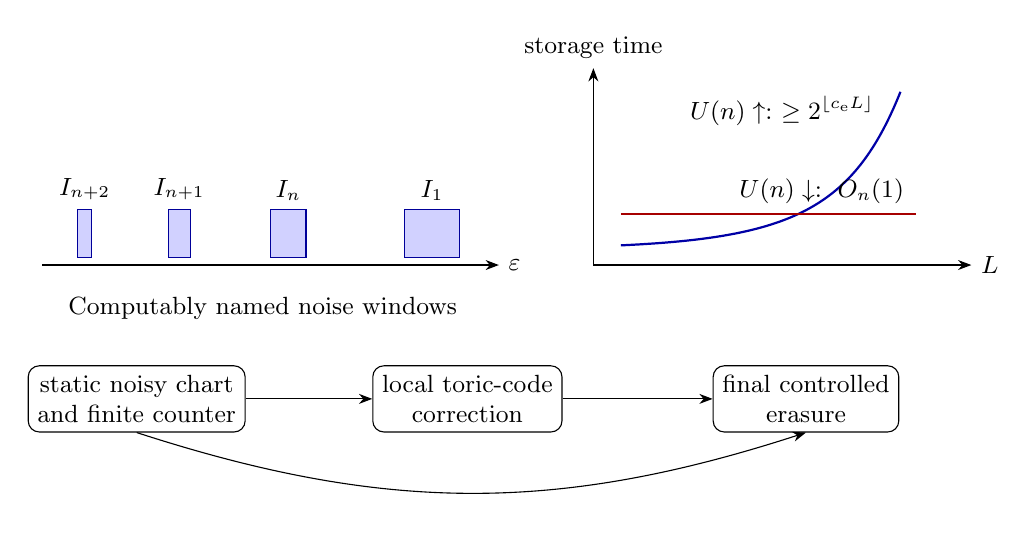
\begin{tikzpicture}[x=1cm,y=1cm,>=Stealth,font=\small]
\draw[->] (0,0)--(5.8,0) node[right]{\(\eps\)};
\foreach \x/\w/\lab in {0.45/0.18/n+2,1.6/0.28/n+1,2.9/0.45/n,4.6/0.7/1}{
 \fill[blue!18] (\x,0.1) rectangle (\x+\w,0.7);
 \draw[blue!60!black] (\x,0.1) rectangle (\x+\w,0.7);
 \node[above] at (\x+\w/2,0.7) {\(I_{\lab}\)};}
\node[align=center] at (2.8,-0.55){Computably named noise windows};
\begin{scope}[shift={(7,0)}]
 \draw[->] (0,0)--(4.8,0) node[right]{\(L\)};
 \draw[->] (0,0)--(0,2.5) node[above]{storage time};
 \draw[thick,blue!65!black] (0.35,0.25) .. controls (2.5,0.35) and (3.3,0.7) .. (3.9,2.2);
 \node[above] at (2.4,1.65) {\(U(n)\uparrow:\ \ge2^{\lfloor c_{\mathrm e}L\rfloor}\)};
 \draw[thick,red!65!black] (0.35,0.65)--(4.1,0.65);
 \node[above] at (2.9,0.65) {\(U(n)\downarrow:\ O_n(1)\)};
\end{scope}
\node[draw,rounded corners,align=center] (a) at (1.2,-1.7){static noisy chart\\and finite counter};
\node[draw,rounded corners,align=center] (b) at (5.4,-1.7){local toric-code\\correction};
\node[draw,rounded corners,align=center] (c) at (9.7,-1.7){final controlled\\erasure};
\draw[->] (a)--(b); \draw[->] (b)--(c);
\draw[->] (a.south) to[bend right=18] (c.south);
\end{tikzpicture}
\caption{Theorem B: exponential guaranteed storage or size-independent
destruction on computable noise windows. Locations, widths and constants
are schematic; the blue curve is a lower bound. Theorem A separately
has the sharp linear scale. Both constructions end each round with a
complete permission-controlled cut.}
\label{fig:story}
\end{figure}

\noindent\textbf{How the medium works.}
For Theorem B, the classical computation is a static chart written once
into a square of side \(\lfloor L/4\rfloor\) and separated from its
periodic copies by vacuum, so it never has to wrap around the torus. A
binary counter along the square's diagonal grants permission to store
for \(2^{\lfloor L/4\rfloor}-1\) rounds. Four further coordinates carry a
closed four-dimensional toric code with a local sweep decoder. Controller
errors are correlated, so we bound them by counting complete witnesses
of each wrong erasure, keeping enough coordinates to tell distinct noise
events apart on the torus. On a halting window every region of the chart
contains a local violation or a wrong rate test, or lies in a square small
enough that its counter expires; permission then dies, and with it every
encoding.

For Theorem D, the same static cap occupies two coordinates and is
protected in two transverse directions. A separate protected classical calendar schedules
a concatenated quantum code along a chain. Folding its cycle into a
segment uses two semantic qubits per site and keeps the interaction range fixed.
The code hierarchy reaches a fixed fraction of the system size. Short
error explanations have consistent source names on the torus; longer
ones have an exponentially small probability. This yields a
stretched-exponential storage guarantee in four dimensions.

For Theorem A, each site runs a noisy classical computation beside a quantum chain.
A second, transversely protected classical field supplies the calendar
for concatenated quantum error correction; higher clocks and programs
remain classical. The computation never reads the noise rate.
Instead, local counters compare how often fresh noise marks appear along
rows of lengths \(2\cdot4^r-1\). On the window \(I_n\) this selects the
depth at which the computation simulates \(U\) on input \(n\). Every
round ends with a controlled erasure of the quantum data at each site
where the computation is not live. For each nonhalting \(n\) and all
\(L\ge L_0(n)\), the computation stays live near the code long enough
for local correction to preserve the stored qubit through
\(\lfloor cL\rfloor\). If \(U(n)\) halts, every chart contains a wrong
gate, and the resulting bounds on paths of quantum dependence destroy
every encoding after a time uniform in system size. Even without halting, the computation needs an
aperiodic chart, which no side-\(L\) torus can carry. By \(200L\) rounds,
continued liveness requires exceptional noise events. Their path bounds
cut the remaining quantum dependence by \(201L+C_0\), outside an event
of exponentially small probability in \(L\). This gives the linear
upper bound and makes the storage scale optimal.

\subsection*{Context and credit}
Undecidable properties of quantum many-body systems include the spectral
gap \cite{CPGW2015} and ground-state phase diagrams. Bausch, Cubitt and
Watson \cite[Theorem~2.1]{BCW2021} construct one continuously
parameterized Hamiltonian with machine-input intervals: nonhalting
gives a gapped product phase on a fixed interval, while halting gives
a critical gapless phase on an interval whose width is specified
existentially. Purcell, Li and Cubitt
\cite{PLC2024} place a single phase boundary at an uncomputable point. Quantum-channel fidelity reachability was already shown
undecidable by Wolf, Cubitt and P\'erez-Garc\'ia \cite{WCPG2011}.
Table~\ref{tab:landscape} locates the operational question studied here.
Our parameter is the rate of independent physical noise following a
fixed circuit, and our negative branch quantifies over encodings into
all its registers. Here the windows are computable on both branches.

\begin{table}[t]
\caption{Closely related results and the observable studied here.}
\label{tab:landscape}
\small\centering
\begin{tabular}{@{}>{\raggedright\arraybackslash}p{0.29\textwidth}>{\raggedright\arraybackslash}p{0.29\textwidth}>{\raggedright\arraybackslash}p{0.34\textwidth}@{}}
\toprule
Work & Setting & Observable\\
\midrule
Cubitt--P\'erez-Garc\'ia--Wolf; Bausch--Cubitt--Watson; Purcell--Li--Cubitt
 & Local Hamiltonians; interaction parameter & Gap and ground-state phase\\[3pt]
Wolf--Cubitt--P\'erez-Garc\'ia & Finite channel collections & Fidelity reached by some channel word\\[3pt]
D\"unnweber--Styliaris--Trivedi; Drechsler--Oreg--Aharonov; Balasubramanian--Davydova--Lake
 & Autonomous noisy quantum memories & Positive storage guarantees\\[3pt]
G\'acs--Reif; G\'acs; Aharonov--Ben-Or; Harrington
 & Hierarchical reliable computation and quantum correction & Protected schedules and encoded gates\\[3pt]
Douglas--Mghirbi & Noisy classical local rules & Ergodicity and computable noise-window selection\\[3pt]
This paper, Theorem A & Fixed seven-gate circuits on \(\Z^3\); physical noise rate & Sharp linear storage, bounded forgetting, exact certification\\[3pt]
This paper, Theorem B & Separate seven-gate W/Q circuits on \(\Z^6\); physical noise rate & Exponential storage lower bound versus size-uniform forgetting on effective windows\\[3pt]
This paper, Theorem D & Seven-gate W circuit on \(\Z^4\); physical noise rate & Stretched-exponential storage lower bound versus size-uniform forgetting on effective windows\\
\bottomrule
\end{tabular}
\end{table}

Autonomous quantum memory under noisy local dynamics predates this
construction, notably the fixed-rule two-dimensional quantum automata
of D\"unnweber, Styliaris and Trivedi \cite{DST2026}, which already
combine G\'acs-style hierarchical classical control with a
measurement-free concatenated quantum code, and the local
toric-code memories of Balasubramanian, Davydova and Lake
\cite{BDL2026}. Both give lifetimes that grow without bound with system
size, in two or three dimensions. The construction of Theorem~A also
combines hierarchical reliable classical computation
\cite{Gacs2001,GacsReif1988} with concatenated quantum fault tolerance
\cite{ABO1999,ABO2008}. The additional conclusions here are an
undecidable noise-window structure with destruction for every encoding;
for Theorem~A, a sharp linear storage scale and exact certification;
for Theorem~B, exponential storage on the undecidable windows
themselves; for Theorem~D, a stretched-exponential guarantee there in
four dimensions under whole-site noise.
Harrington's hierarchical local decoder
\cite{Harrington2004} is an early quantum-memory precedent. The exponential constructions use the toric-code and sweep lineage of
Dennis, Kitaev, Landahl and Preskill \cite{DKLP2002}, Ahn
\cite{Ahn2004}, Kubica and Preskill \cite{KubicaPreskill2019}, and
Vasmer, Browne and Kubica \cite{VBK2021}. Particularly close comparisons are
the classical-to-quantum memory correspondence of Drechsler, Oreg and
Aharonov \cite{DOA2026} and the cubical sweep fault-tolerance theorem of
Ponarovsky \cite{Ponarovsky2026}. We prove the source-dependent estimate
needed for this medium rather than invoking a threshold for independent
faults: the controller induces correlated erasures.

The classical computational controller builds on our preprints on
fixed-noise ergodicity, undecidable phase diagrams, and an uncomputable
noise diagram \cite{DMFixed2026,DMPhase2026,DMNoise2026}. Those works
supply the finite computational charts and classical probability
estimates. Version 1.0.0 of this paper \cite{DMQuantum2026} already proved the
linear quantum bridge and a designed exponential window. Version 2.0.0 \cite{DMQuantumV200} already supplies the static cap,
canonical initializer, correlated-source method and six-dimensional
Theorem B, together with Section~\ref{sec:quantum}'s real code gadgets
and Section~\ref{sec:forgetting}'s full-channel sharing argument.
Theorem D combines those published ingredients, including the
private-port dispatcher of Section~\ref{d:dispatch} and the fold of
virtual cycles into physical sheets with sheet-typed fault labels from
Appendices~\ref{sec:fold-controls}--\ref{sec:folded}, with whole-state
periodic calendar resets, exclusive port selection and a torus source
analysis that controls aliases of the same physical fault. Its new
conclusion is beyond-polynomial storage on the undecidable windows in
four dimensions for whole-site noise.

Appendix~\ref{sec:coexistence} retains a separate four-dimensional
construction. Proposition~\ref{p:coexistence} gives one independent-qubit
medium with the same seven gates, an uncomputable storage diagram, and a
reserved, designed and decidable window storing a qubit for
\(2^{\lfloor c_{\exp}L\rfloor}\); its universal nonhalting windows have
linear storage. Version 1.0.0 left exponential storage on the undecidable
windows themselves open; Theorem B provides it, in six dimensions and for
both noise models. Its proof uses the deterministic finite-torus
machinery of Lemma~\ref{x:exponential}.

\paragraph{Changes in 2.0.0.}
Theorem B adds exponential storage on the undecidable windows for
separate six-dimensional media in both noise models. Theorem A and
the four-dimensional designed-window result are retained. The new
proof, a coarse lifetime upper bound and exponential-horizon
certification are in Section~\ref{sec:exponential}; the discussion
states the remaining dimensional and matching-lifetime questions.

\paragraph{Changes in 2.1.0.}
Theorem D lowers the dimension of beyond-polynomial storage on the
undecidable windows from six to four for whole-site noise.
Section~\ref{sec:four-dimensional} gives the construction and proof;
Appendices~\ref{app:f4-calendar}--\ref{app:f4-sources} prove the added
calendar, folded-dispatch and torus-source lemmas. Theorems A and B and
Appendices A--C retain their previous mathematical statements.
Appendix~\ref{app:lean} adds Lean verification of Lemma~\ref{f:bell}
and the printed conditional abstraction of Theorem~\ref{a:complete}.

\subsection*{Reading guide}
Section~\ref{s:model} states the model and full quantifiers.
Sections~\ref{sec:controller} and~\ref{sec:compilation} give the classical
selector and exact physical implementation. Section~\ref{sec:quantum}
proves three-dimensional storage, including the gadget support bound,
source counting and decoding at every requested time.
Sections~\ref{sec:forgetting} and~\ref{sec:ceiling} prove the two
all-encoding bounds; Section~\ref{a:certification} proves certification.
Section~\ref{sec:exponential} proves Theorem B, including its static
initializer, physical-name density bound, source law, quantum recovery
and full-algebra negative branch. Computability readers can proceed
from Theorem A to certification, or from Theorem B to its static
alternative and final channel argument.
Quantum-information readers can take the explicitly stated classical
chart interface as an input. The folded-code and exponential-coexistence
proofs are in Appendices~\ref{sec:fold-controls}--\ref{sec:coexistence}.

Section~\ref{sec:four-dimensional} can be read after the code and
normalizer lemmas of Section~\ref{sec:quantum} and the static cap of
Section~\ref{sec:exponential}. Its dependency tables specify the
constant order; its appendices contain the new source and fold proofs.

\section{Model, fidelity and detailed three-dimensional theorem}\label{s:model}
This section fixes the local circuit model, the two noise models and the fidelity and lifetime used throughout. It states Theorem~\ref{thm:detailed}, the detailed form of Theorem~\ref{thm:main}.

Universality supplies a total computable compiler from program codes \(e\) to inputs \(n\) such that \(U(n)\) halts exactly when program \(e\) halts on input \(0\) (Section~\ref{a:certification}). Each construction has nonempty open windows \(I_n\) with rational endpoints. The total computable noiseless encoder depends on \((n,L)\), and the total computable noiseless decoder on \((n,L,t)\). On a halting window the forgetting bound holds for all encoders and decoders on the entire register, for every \(L\), every rate in \(I_n\), and every integer \(t\) at or above the cutoff \(C_{n,\eta}\) in the corresponding theorem. Time counts rounds in Theorems~\ref{thm:exponential} and~\ref{thm:main} and elementary layers in Theorem~\ref{thm:four-dimensional}.

\subsection{Terminology}
We call the registers of the rule before physical compilation \emph{semantic registers}. A site can hold several such registers and the extra wires used to implement them. Table~\ref{tab:terms} gives the recurring terms.

\begin{table}[!tb]
\caption{Terminology used in the construction and the proofs. The source vocabulary (bin, star, seed, witness, certificate, charge, image, catalogue and overlay) is explained in Section~\ref{c:named-sources}.}\label{tab:terms}
\small\centering
\begin{tabular}{@{}>{\raggedright\arraybackslash}p{.23\linewidth}>{\raggedright\arraybackslash}p{.51\linewidth}>{\raggedright\arraybackslash}p{.19\linewidth}@{}}
\toprule Term & Meaning & Defined in\\\midrule
Selector and chart & Rate-selecting classical controller and its locally checked space-time diagram. In six and four dimensions the chart is a static patch. A live letter is a nonbottom symbol. & Sections~\ref{c:chart}, \ref{sec:exponential} and~\ref{sec:four-dimensional}\\\addlinespace[3pt]
Cap, profile and death flag & Finite static computation patch with a diagonal overflow counter. Its per-site profile is \(\mathsf{pr}\). The flag \(\mathsf d\) records whether erasure has been triggered at or has propagated to a site. & Section~\ref{sec:exponential}\\\addlinespace[3pt]
Replica and sampling lane & A replica is one transverse displacement supplying one vote. A sampling lane follows a row by copying a register that samples noise. One such copying interval is called a ride. & Sections~\ref{c:chart} and~\ref{v:parameters}\\\addlinespace[3pt]
Censor & Local statistical test that can replace a computation symbol by \(\bot\). & Section~\ref{sec:exponential}\\\addlinespace[3pt]
Storage-enable bit and cut & In six and four dimensions the storage-enable bit controls conditional reset. A cut removes incoming dependence through that reset. & Sections~\ref{sec:exponential}, \ref{sec:four-dimensional}\\\addlinespace[3pt]
Conditional reset and mixed ancilla & Controlled swap with a fresh maximally mixed ancilla, then reset of that ancilla. In the clean circuit a triggered cut replaces each data qubit by \(I/2\). & Section~\ref{sec:compilation}\\\addlinespace[3pt]
Hidden cover, realization and rate bound & A hidden cover adds letters to projected chart geometry so legality is local. A realization compiles the rule for one noise model. A rate bound is an upper bound on a fault or refresh probability. & Sections~\ref{c:chart} and~\ref{sec:compilation}\\\addlinespace[3pt]
Dirty location & Circuit location touched by a fault or by a wrong controller output. & Section~\ref{d:dispatch}\\\addlinespace[3pt]
Sheet and dispatch & A sheet is one affine branch of a folded code. Dispatch is the selection and execution of a local gate through its ports. & Section~\ref{d:dispatch}, Appendices~\ref{app:f4-dispatch} and~\ref{sec:folded}\\\addlinespace[3pt]
Clock and exclusive dispatcher & The clock is a classical scheduling field. The dispatcher uses exclusive ports to implement the chosen gate. & Section~\ref{d:calendar-section}, Appendices~\ref{app:f4-calendar} and~\ref{app:f4-dispatch}\\
\bottomrule
\end{tabular}
\end{table}
Table~\ref{tab:geometry} lists the coordinate roles. In the six-dimensional construction \(u\) denotes the patch coordinates and \(P\) the four code coordinates. In the four-dimensional construction \(\mathsf C\) is the computation field and \(\mathsf S\) the clock field. The chain coordinate is \(\sigma\), the clock block length is \(P_{\rm cal}\), the simulation period is \(T_{\rm cal}\), and \(k\) is the concatenation depth. The window bound \(w_n\) is on bin height and \(\alpha_4\) is the storage exponent.

\begin{table}[!tb]
\caption{Coordinate roles. The second coordinate \(t-i\) of the three-dimensional computation is a space-time coordinate.}\label{tab:geometry}
\centering\small
\begin{tabular}{@{}l>{\raggedright\arraybackslash}p{.32\linewidth}>{\raggedright\arraybackslash}p{.49\linewidth}@{}}
\toprule Circuit & Computation & Quantum data\\\midrule
6D (A) & Static patch in \((u_x,u_y)\) & Four-dimensional toric code in \((P_1,P_2,P_3,P_4)\)\\\addlinespace[3pt]
4D (B) & Static patch in \((x,y)\) & Chain along \(\sigma\), folded into two internal roles\\\addlinespace[3pt]
3D (C) & Space-time diagram in \((i,t-i)\) & Chain along \(\sigma\)\\\bottomrule
\end{tabular}
\end{table}

The separate four-dimensional circuit of Appendix~\ref{sec:coexistence}
uses the four-sheet geometry of Appendix~\ref{sec:folded} and a separate
closed-code track. The recurring constants are explained in
Appendix~\ref{app:code-estimates}.

\subsection{Local circuits and two noise models}\label{s:local-circuits}
Each construction has a fixed local register and a fixed repeating schedule. We begin with the three-dimensional register convention; the later theorems specify their other lattice dimensions.
Let \(\mathbb T_L^3=(\Z/L\Z)^3\). One physical site carries
\(\mathcal H_x=(\mathbb C^2)^{\otimes N}\), where \(N\) is one fixed
finite integer. It includes every data, controller, sensor, transport
and work qubit. A gate layer is a translated product of gates on
disjoint internal tensor factors. Several such gates can meet the same
physical product site on different factors. Every gate has at most
three input qubits and uses one of finitely many displacement templates, independent of \(n,L,\eps\).

\begin{definition}[Whole-site depolarizing noise, WS]\label{def:noise-w}
Following each gate layer, independently at each physical site, apply
\begin{equation}\label{eq:site-noise}
 \mathcal D_{\eps,x}(\rho)
 =(1-\eps)\rho+\eps\,\frac{I_x}{2^N}\otimes\Tr_x\rho.
\end{equation}
\end{definition}
\begin{definition}[Independent single-qubit depolarizing noise, Q]\label{def:noise-q}
In realization \(\mathrm Q\), independently on every wire after every layer, apply
the one-wire channel \(\rho\mapsto(1-\eps)\rho+\eps I/2\), tensored with the identity on all other wires.
\end{definition}
In both realizations the same
physical rate follows preparation, dephasing, reset, and idle layers.
\(\mathrm{WS}\) and \(\mathrm Q\) are separately compiled fixed circuits; their dimensions,
schedules and physical windows may differ. Gates in a layer are disjoint
on qubits and may share physical sites. All spatial gates have fixed
finite range, which need not be one lattice spacing. The gate list is
\[
 \{X,H,\mathrm{CNOT},\mathrm{Toffoli},R_0,D_Z,I\}.
\]
The unitary subset contains the computationally universal pair Toffoli and Hadamard \cite{Aharonov2003,Shi2003} (universality here is the real-amplitude simulation of complex computation with one extra qubit, in the sense of \cite[Definition~3 and Theorem~2]{Aharonov2003}). Here \(R_0(\rho)=|0\rangle\langle0|\Tr\rho\) and \(D_Z\) is complete
computational-basis dephasing; a measurement is a \(D_Z\) whose outcome
stays on a basis-valued wire.
\Needspace{7\baselineskip}
\begin{definition}[Round channel]\label{def:round}
Repeating the fixed circuit defines a round channel \(\Lambda_{L,\eps}\).
One application is one round. If the period is \(J\) elementary layers,
then at aligned times \mbox{\(t_{\rm layer}=Jt_{\rm round}\)}.
For Theorem~\ref{thm:four-dimensional}, including Theorem~\ref{f4:detailed},
bound~\eqref{f4:lifetime-upper}, Table~\ref{tab:results} and
Corollary~\ref{cor:window-undecidable}, fidelity and lifetime are measured
in elementary layers. In this convention use \(\Lambda^{(t)}_{L,\eps}\),
the channel of the first \(t\) noisy layers starting at a round boundary,
in Definitions~\ref{def:fidelity} and~\ref{def:lifetime}. Convert round
quantities in the proof at aligned times using the period.
Unless elementary layers are specified, \(t\) counts rounds.
\end{definition}

\subsection{Storage fidelity}
CPTP means completely positive and trace preserving.
\begin{definition}[Entanglement fidelity]\label{def:fidelity}
Let \(\beta=|\beta\rangle\langle\beta|\), with
\(|\beta\rangle=(|00\rangle+|11\rangle)/\sqrt2\). The reference qubit
is never acted upon. For CPTP encoding and decoding maps \(\cE,\cD\), put
\begin{equation}\label{eq:fidelity}
 F(\cE,\cD;L,t,\eps)=
 \langle\beta|[\mathrm{id}\otimes
 (\cD\Lambda_{L,\eps}^t\cE)](\beta)|\beta\rangle,
 \qquad F^*_{L,\eps}(t)=\sup_{\cE,\cD}F(\cE,\cD;L,t,\eps).
\end{equation}
This is entanglement fidelity for the maximally mixed logical qubit.
\end{definition}
The supremum allows arbitrary encodings into the entire physical
algebra, including work and controller registers, with no persistent
outside quantum memory. \begin{definition}[Memory lifetime, or storage time]\label{def:lifetime}
Let
\[
 \tau_{L,\eps}=\sup\{t\in\N:F^*_{L,\eps}(t)\ge7/8\}.
\]
\end{definition}
Optimal fidelity is nonincreasing in \(t\). A later decoder composed with the intervening channel is a decoder at the earlier time. The passing layer times
therefore form an initial segment, and the passing round times are
precisely the aligned times in that segment. For a period of \(J\)
layers, the optimized integer lifetimes satisfy
\(\tau_{\rm round}=\lfloor\tau_{\rm layer}/J\rfloor\) when finite,
and are both infinite otherwise. Our explicit decoder can depend
on \(t\), as well as \(n,L\), and remains independent of the rate.


\begin{definition}[Storing and forgetting windows]\label{def:windows}
A \emph{rate window} is a nonempty open interval with rational endpoints. For a specified encoder family, decoder family, horizon and size threshold, a \emph{storing window} is one on which the stated fidelity guarantee holds at every rate and every indicated size and time. A \emph{forgetting window} is one on which, for every \(\eta>0\), the optimal fidelity is at most \(1/2+\eta\) after a finite time uniform in size and rate. A \emph{scalable-memory rate} is one with \(\sup_L\tau_{L,\eps}=\infty\). A \emph{scalable-memory window} consists entirely of such rates. Nonhalting and halting windows are indexed by \(n\) with \(U(n)\uparrow\) and \(U(n)\downarrow\), respectively. The theorems give storing windows with fidelity \(15/16\); certification tests the weaker bound \(7/8\). The limiting benchmark \(1/2\) is the largest entanglement fidelity attainable by a measure-and-prepare qubit channel.
\end{definition}

\begin{theorem}[Detailed form of Theorem~\ref{thm:main}]\label{thm:detailed}
For each of \(\mathrm{WS}\) and \(\mathrm Q\) there are a computably specified,
translation-invariant, time-periodic circuit as above, a computable sequence
of disjoint nonempty rational open intervals
\(I_n\subset(0,1)\), a rational \(c>0\), and computable thresholds
\(L_0(n)\), with \(c\) independent of \(n\), and the following properties.
\begin{enumerate}
\item There are total computable maps \(\cE_{n,L}\) and
\(\cD_{n,L,t}\), independent of \(\eps\) and of whether \(U(n)\)
halts. If \(U(n)\uparrow\), then for every \(\eps\in I_n\),
\(L\ge L_0(n)\), and every integer \(0\le t\le\lfloor cL\rfloor\),
\(F(\cE_{n,L},\cD_{n,L,t};L,t,\eps)\ge15/16\).
\item If \(U(n)\downarrow\), then for every \(\eta>0\) there is
\(C_{n,\eta}<\infty\) such that
\(F^*_{L,\eps}(t)\le1/2+\eta\) for every \(L\),
\(\eps\in I_n\), and \(t\ge C_{n,\eta}\).
\item There are computable constants \(A,a>0\), \(b\in\N\), \(C_0\ge2\)
and \(L_1\), all independent of \(n\), such that for every \(n\), every
\(\eps\in I_n\) and every \(L\ge L_1\), with \(s_L=201L+C_0\),
\[
 \Lambda_{L,\eps}^{s_L}=(1-r_L)\Phi^{\rm EB}_{L,\eps}+r_L\mathcal B_{L,\eps},
 \qquad r_L\le q_L\le AL^be^{-aL},
\]
where \(\Phi^{\rm EB}_{L,\eps}\) is entanglement breaking (EB) and
\(\mathcal B_{L,\eps}\) is a channel. In particular
\mbox{\(\|\Lambda_{L,\eps}^{s_L}-\Phi^{\rm EB}_{L,\eps}\|_\diamond\le2q_L\)} and
\(F^*_{L,\eps}(t)\le1/2+q_L/2\) for every \(t\ge s_L\).
\item The predicate requiring the explicit fidelity to be at least
\(7/8\) for every integer \(L\ge L_0(n)\), integer
\(0\le t\le\lfloor cL\rfloor\), and rational \(\eps\in I_n\)
holds exactly when \(U(n)\uparrow\) and is \(\Pi^0_1\)-complete.
Every finite test is an exact rational comparison.
\end{enumerate}
\end{theorem}

If \(U(n)\) never halts, these bounds give
\(\lfloor cL\rfloor\le\tau_{L,\eps}<201L+C_0\) for every \(\eps\in I_n\)
and every \(L\ge L_C(n):=\max\{L_0(n),L_1,L_2\}\). Here \(L_2\) is a
computable size beyond which \(AL^be^{-aL}<3/4\). One can search beyond
\(b/a\), where this bound decreases, until a certified upper estimate
is strictly below \(3/4\). Thus
\(\tau_{L,\eps}=\Theta(L)\), uniformly across the window. On halting windows the lifetime is
uniformly bounded in \(L\). These halting-side times are finite but not
computable from \(n\): for each fixed rational \(0<\eta<3/8\), no total
computable function of \(n\) can serve as \(C_{n,\eta}\) in part (ii)
(Corollary~\ref{a:time}). Computable windows and their rational midpoints
already suffice for the undecidability assertion. The scope is as in Section~\ref{intro:scope}.

For fixed \(L\) and \(\eps>0\), complete replacement of every physical
factor at the last layer of a round has probability
\(p_{L,\eps}=\eps^{L^3}\) in \(\mathrm{WS}\) and
\(p_{L,\eps}=\eps^{NL^3}\) in \(\mathrm Q\). If it has occurred, the output is
independent of the input. Thus
\begin{equation}\label{eq:finite-reset}
 F^*_{L,\eps}(t)\le\frac14+\frac34(1-p_{L,\eps})^t.
\end{equation}
This also controls the finitely many small volumes omitted from
asymptotic estimates.

Sections~\ref{sec:controller}--\ref{a:certification} prove Theorem~\ref{thm:detailed}. Section~\ref{sec:controller} constructs the classical selector and Section~\ref{sec:compilation} compiles it and fixes the constants. Section~\ref{sec:quantum} proves (i), Section~\ref{sec:forgetting} proves (ii), Section~\ref{sec:ceiling} proves (iii), and Section~\ref{a:certification} proves (iv).

\section{A classical computation that controls erasure}\label{sec:controller}

The classical part of the medium determines when local quantum data may
remain. Its input is the noise distribution itself. We specify the classical
facts that are imported from the authors' preprints, then prove the interfaces
needed for quantum storage. In particular, a classical loss of memory will
be converted into a statement about actual quantum dependence, rather than
used as a substitute for it.

\subsection{The selector and its computational chart}
For the three-dimensional construction use coordinates
\(z=(i,P_1,P_2)=(i,\sigma,z_3)\in\Z^3\).
There is one selector, denoted \(C_{\rm sel}\). In the separate
four-dimensional construction of Appendix~\ref{sec:fold-controls},
a copied coordinate \(Q\) and four signed orientations are added.
Formulas involving \(Q\) below omit that coordinate in three dimensions.
Its chart coordinates at round \(t\) are
\[
 (x,y)=(i,t-i).
\]
Thus the west and south chart neighbours are actual previous-time sites
\((i-1,t-1)\) and \((i,t-1)\), respectively. Set
\begin{equation}\label{eq:c-boxes}
 S_0=[0,15]^2,\qquad S_1=160e_1+S_0,\qquad
 S_2=160e_2+S_0,\qquad K=256,\quad h=512.
\end{equation}
Intervals of integers are understood in these formulas. A chart alphabet
\(\mathcal A\), with an added symbol \(\bot\), has a partial completion
map \(g\) from west and south letters. A chart letter is live when it differs from \(\bot\). The map is functional: there is at
most one completion. It is bottom-spreading, so a live completion requires
two live inputs. The ordinary proposal at \((i,P,t)\) is the unique letter
proposed by at least \(h\) of the \(3K\) providers in
\(S_0\cup S_1\cup S_2\); if there is none, it is \(\bot\).
A provider uses both logical inputs at its own transverse displacement.
Two different letters cannot both receive \(h\) votes.

The retained first chart coordinate is an erasure of this ordinary proposal;
a second coordinate records the ordinary proposal. Additional helper
coordinates test the scale of the noise and may replace the first coordinate
by \(\bot\). These tests compare short rides along chart rows with recent
rides, meaning helper-copying intervals, of length
\begin{equation}\label{eq:c-scales}
 \ell_r=2\cdot4^r-1,\qquad W=\lfloor C/\mu\rfloor.
\end{equation}
Here \(\mu\) is the aggregate refresh rate and \(C\) is a fixed rational
constant selected later. The physical rule does not read either number.
The value \(W\) is used only to analyze its experiments. A fixed bank of
\(B\) helper lanes supplies the votes. Each binary-coded helper has one
low code, one unknown code and 126 high codes. The chart history has fixed
depth \(T=1024\), with its local history consistency tests included in the
ordinary completion map.

The following classical input is used: the chart and machine construction
of \cite[Proposition~4.3, Lemmas~4.1--4.2 and~11.2--11.3]{DMNoise2026}, its
finite-history boundary-path estimate
\cite[Lemma~11.6]{DMNoise2026}, its intrinsic experiment and source bounds
\cite[Lemmas~6.1--6.3 and~10.4]{DMNoise2026}, and the scaffold parent and
soundness lemmas \cite[Lemmas~A.3 and~A.2]{DMPhase2026}. The provider
method originates in \cite[Theorem~2.1]{DMFixed2026}. A computation board
is a finite grid carrying successive configurations of the fixed machine;
legality means its local transition and boundary constraints hold. Its
row flag is a binary chart label. A critical gate is the helper test at
the bottom end of a row at one of the two depths specified below.

\begin{proposition}[Classical chart interface]\label{c:selector-import}
There is an effective finite chart alphabet and a fixed finite helper rule
with the following properties. For a universal machine \(U\), choose
\(a=n+n_0+1\) and the nominal window
\begin{equation}\label{eq:c-window}
 J_n=\left(\frac{2C}{\ell_a},\frac{21C}{10\ell_a}\right).
\end{equation}
Throughout this window, \(\ell_{a-1}<W\), \(2W\le\ell_a\), and
\(W\le4^a-1\). If \(U(n)\) does not halt, the chart has a canonical
projected geometry with cutoff \(a\) with a legal finite-state cover and legal
finite computation boards. If \(U(n)\) halts, every full chart has a wrong
critical gate of one of two types: a short depth-\((a-1)\) gate with flag
zero, or a long depth-\(a\) gate with flag one.

The canonical projected geometry is computable on signed coordinates.
Its helper copy characteristic preserves the base chart row of each lane.
For a fixed candidate critical gate and a deterministic finite footprint,
the intrinsic experiment estimates (the bounds \(u_B,z_B,w_B\) of
\eqref{eq:c-eta}) and the finite-history boundary-path estimates
(\cite[Lemma~11.6]{DMNoise2026}) hold with constants uniform on \(J_n\). On halting, the finite
motif radius needed for these estimates is found by a terminating search
through finite locally compatible patches.
\end{proposition}

Here the finite motif search rejects a patch when it contains either of
the two wrong-gate rides. If arbitrarily large survivors remained,
compactness would give a full chart with neither ride, contrary to the
machine construction. This explains both termination on halting and why
the search is not a halting decision procedure. The effective chart cover
uses the NE consequence of the strongly deterministic substitution-cover
theorem of Le Gloannec and Ollinger \cite{LGO2012}: the limit set of a \(2\times2\) substitution has
an effective finite cover whose full west and south neighbours determine
at most one tile. The limit set here consists of full-plane colourings
admitting arbitrarily deep compatible desubstitutions. The canonical
projected geometry belongs to it. One can see this by using its finite
output automaton as a state substitution, translating state quadrants
far into the positive quadrant, and taking compatible limits at every
substitution depth. The finite collar and cutoff constraints only reject
cover completions, so they preserve functionality.

The positive-input convention fixes the window labels exactly.
Let \(V(m)=U(m-1)\), \(m\ge1\). If the scan's first zero is
\(j_*\), it accepts \(j_*+2=2^e\), writes \(e\) tokens and
consumes \(n_0+1\) of them before calling \(V\) on
\(m=e-n_0-1\). At cutoff rank \(a\),
\(j_*=2^{a+1}-2\), so \(m=a-n_0=n+1\) and the simulated
computation is exactly \(U(n)\). The finite scan machine is built
after \(n_0\) is fixed.

\subsection{Total finite initialization}\label{subsec:c-initialization}
A global hidden-cover choice need not be computable. Only a finite legal
choice is required by the encoder.

\begin{lemma}\label{c:initialization}
From \((n,L)\) and a declared finite time horizon one can compute an initial
controller word, without the noise rate or a halting answer. On a
nonhalting input it agrees with a correct-cutoff reference on the entire
required initial, history, helper and future cone. Its helper initialization
satisfies the same short upper and recent-long lower experiment bounds as
the classical interface.
\end{lemma}
\begin{proof}
Compute the canonical projection, cutoff, and finite payload on a
square containing the
whole cone, every initial history slot, and all fixed lane and collar
offsets. Exhaust the finite list of cover-letter assignments on that
square, imposing the computed projection and every local constraint.
Return the first successful assignment, with a fixed fallback if the list
is empty. The algorithm always terminates. On nonhalting, a global cover
of the projected reference supplies a successful finite assignment.
Functionality forces its future on the smaller cone. Assignments for
different sizes need not be restrictions of a common hidden cover.

Initialize helpers deterministically: use low on reference flag-one rows
and high on flag-zero rows. Each helper field must use its own base row.
The copy characteristic preserves that row, even when the physical field
index changes its offset. On a short ride, a low initial value can only
remove a contribution until a genuine future mark is seen; hence its
upper bound is preserved. On a long ride, a high initial value dominates
the recent-\(W\) comparison until \(W\) genuine future atoms have become
available. Thereafter the latest genuine mark gives the usual comparison.
This argument also covers an experiment crossing time zero.
\end{proof}

\subsection{Named sources under layer noise}
The compilation described in Section~\ref{sec:compilation} has a useful
classical consequence. Let \(A_{z,t}\) record any internal fault at site
\(z\) in round \(t\), and let \(E_{z,t}\) be its independent aggregate
refresh. Put
\[
 H_{z,t}=A_{z,t}\lor E_{z,t},\qquad p=\Pr(H_{z,t}=1)\le2\mu.
\]
The family \(H\) is independent on physical site/round names. One
name can corrupt arbitrary outgoing copies of that site's old word and
its own new output. Copies from the same word may disagree. Seed both
formal occurrences \((z,t-1)\) and \((z,t)\) from the single name
\((z,t)\). Let \(M^0\) be the least finite-start marked field obtained by
adding these seeds and marking a nonfresh vertex whenever marked ordinary
parents occur in two distinct provider boxes. Nonexistent pre-zero sources
are omitted.

To formulate the positive source estimate, use base characteristics and
bins of length \(W\). A source label is
\(\lambda=(i-t,P+58t(1,1),Q,\lfloor t/W\rfloor)\).
Geometric roles annotate the witness and do not split one source label.
Source labels do not count independent microscopic faults: an intrinsic test
can involve many physical atoms. All occurrences with the same label
are kept together.

\begin{proposition}[Joint source law]\label{c:source-law}
There are fixed finite support lists and computable overlap divisors
\(D_{\rm bin},D_{\rm hist}\), independent of \(W,n\), such that the
following holds. Let \(O_\lambda\) mean an internal fault in the complete
hardware support of an experiment in label \(\lambda\), and suppose
\(\Pr(O_\lambda)\le\alpha\). For any \(g\) distinct source labels,
\begin{equation}\label{eq:c-gamma}
 \Pr(\hbox{all labels have a raw or intrinsic exception})
 \le\gamma_0^g,\qquad
 \gamma_0\le\sqrt{2C}+\eta_B^{1/6}
                  +\alpha^{1/(2D_{\rm bin})},
\end{equation}
where
\begin{align}\label{eq:c-eta}
 u_B&=2^{-\lfloor3BC/100\rfloor},&
 z_B&=2^{-\lfloor BC/3\rfloor},&
 w_B&=2^{-\lfloor BC^2/50\rfloor},\notag\\
 \eta_B&=\frac{3u_B}{1-4z_B}+2w_B,
 &4z_B&<1.
\end{align}
For \(m\) distinct historical fixed-gate tests the augmented intrinsic
intersection has probability at most \(\theta^m\), where
\begin{equation}\label{eq:c-theta}
 \theta=\eta_B+\alpha^{1/D_{\rm hist}}.
\end{equation}
A larger common divisor can be used for boundary tests.

Every erroneous initialized controller reading has a finite acyclic
backward derivation through ordinary two-box supports, helper corridors,
or these source labels. In characteristic coordinates helper corridors
preserve all five potentials used by the quantum proof. Collapsing them
leaves a finite set of roles and bounded bin shifts.
\end{proposition}
\begin{proof}
The binary helper coding changes the upper fresh-mark prefactor to
\(127/128\) and the lower to \(126/128\ge .98\). On a short depth
\(a-1-r\) ride the mean is less than \(.53C4^{-r}\); the voting
threshold is at least \(.75C\). On a recent long ride the mean exceeds
\(.9C\), while the threshold is at most \(.8C\). The exponential
moment bounds for these two Bernoulli comparisons give \(u_B,z_B,w_B\);
summing short depths gives the geometric denominator in
\eqref{eq:c-eta}. These are the intrinsic estimates in the classical
interface, with conservative binary-coding prefactors.

Raw \(H\) bins have disjoint physical atoms and probability at most
\(pW\le2C\). Baseline intrinsic tests use only \(E\) and fresh baseline mixed-helper
marks. On \(A=0\) these are the actual marks; dirty outputs on \(A=1\)
are Byzantine and charged to the overlay. Only
\(E\cap\{A=0\}\) is used to infer an actual uniform product. Distinct characteristics own disjoint lane characteristics, and
every third bin has disjoint intrinsic support; hence \(g\) specified
baseline tests cost at most \(\eta_B^{g/3}\).

An internal exception includes the full support of every short ride and
recent experiment in the bin. Its atoms lie on a fixed characteristic
translate list and in a fixed number of adjacent bins, so there are at
most \(h_0W\) atoms. Its probability is at most \(h_0W\nu\), where
\(\nu=\Pr(A=1)\). Supports can overlap only at differences from a fixed
finite list. A proper colouring of that overlap graph, with at least
one more colour than its degree, yields
\(\Pr(\bigcap O_\lambda)\le\alpha^{g/D_{\rm bin}}\).
The \(E\) and \(A\) families are independent. Combine their intrinsic
bounds, then use Cauchy--Schwarz against the raw family, which overlaps
both. Expanding the possible source types gives exactly
\eqref{eq:c-gamma}. Different \(Q\) copies within one selector have disjoint physical
innovations; their copy names remain part of the label.

For historical tests, write an atom of a ride starting at chart endpoint
\(g=(g_x,g_y)\), time \(b\), and provider \(P_b\) as
\[
 x=g_x-\ell+\delta_x,\quad y=g_y+j+\delta_y,
 \quad P=P_b+58\ell(1,1)+\delta_P,
 \quad s=b-\ell+\delta_t.
\]
The offset \(\delta\) ranges over a fixed support list. Equality of a
physical atom between two tests implies
\[
 b-b'=(\delta_x-\delta_t)-(\delta'_x-\delta'_t).
\]
Thus the difference of their start times lies in a fixed finite list,
independently of \(W\) and of the provider path. Colouring gives
\(D_{\rm hist}\), and independence of the baseline and internal
families gives \eqref{eq:c-theta}. This remains a fixed-support statement
when a later union bound chooses paths after seeing the noise.

Finally, a wrong clean ordinary output has more than \(K\) failing
providers, so wrong inputs occupy two boxes. A helper error either has
an intrinsic exception or follows its unique copy characteristic to a
wrong driver. That corridor preserves its characteristic potentials;
a driver step then makes positive progress. Expanding the fixed-depth
query and ordinary rule strictly decreases the formal history order,
ending at a named source or the ideal initial reference. This proves
finiteness and acyclicity. The projected role list is independent of the
lane length because its fixed offsets cancel along a complete corridor.
\end{proof}

\subsection{All-start halting estimates}
We next remove the intended initialization. First work in one selector
marginal; the resulting events dominate all initial words at once.

\begin{lemma}[Finite-age coherence]\label{c:coherence}
Let \(\mathsf H(z,t)\) mean that an ordinary parent of \((z,t)\)
belongs to \(M^0\), and let \(D_s(z,t)\) be the event that a backward
ordinary path of length \(s\) has at least \(\delta s\) such positions,
where \(\delta=1/1404\). Outside the corresponding two \(D_s\) events,
two unmarked live readings at the same logical position and time,
provider distance \(d\), and age at least \(s\ge\max(1,2d)\) agree. A clean
child check and this equality certify local west/south compatibility.
At a sufficiently small computable source rate,
\(\Pr(D_s(z,t))\le A\exp(-as)\) in an unwrapped finite cone.
\end{lemma}
\begin{proof}
At an unmarked root at most one provider box contains marked ordinary
inputs. Therefore at least \(h-K=256\) successful providers read actual
unmarked words. When neither comparison root has \(\mathsf H\), pair
providers by a unit shift reducing their signed \(\ell^1\) distance.
There are \(3\cdot16\cdot15=720\) pairs. At most
\(2(3K-h)=512\) fail one of the two checks, leaving a reducing pair.
Functionality selects a common conflicting west or south input. At an
exceptional step choose any clean successful provider at each root;
functionality still selects a conflicting logical input, and provider
distance increases by at most 350. After one step both readings are
actual first-coordinate words. Distance-zero conflict is then impossible,
including at time zero. With fewer than \(2\delta s\) exceptional
steps the final distance is strictly less than
\[
 d-s+351(2\delta s)=d-s/2,
\]
a contradiction. For compatibility use one clean child provider, and
compare its two actual old inputs with the chosen reference inputs.

For the probability bound, use poles
\(3(\chi_1+\chi_2),-3\chi_1,-3\chi_2\), where
\(\chi=P+58t(1,1)\). Good gains are 129, the largest loss is 351,
and a grouped old/new name has total oscillation 696. The balanced
terminal-arm count of Lemma~\ref{q:frontier} gives fewer than \(17f\) positive edges for \(f\)
distinct names; the conservative budget \(64f\) also covers the group
stars. Attach complete contours at the marked parents along the selected
path. Retain each complete contour and restart at least two times before
its earliest physical name. Disjoint source slabs then cover at most
\(68F\) path positions with \(F\) distinct names. Thus
\(F\ge\lceil\delta s/68\rceil\), and the path and contours form a
connected graph of \(O(F/\delta)\) edges. A fixed finite-degree graph has
at most \(K_\delta^F\) such rooted annotated graphs. Summing their
probabilities \(p^F\) proves the estimate at a small enough fixed rate.
\end{proof}

\begin{proposition}[Late unmarked liveness]\label{c:late-live}
If \(U(n)\) halts, there are finite \(A_n,a_n>0\), uniform for
\(\mu\in J_n\), such that
\begin{equation}\label{eq:c-late}
 \Pr\{\text{some initial word gives an unmarked live reading at }(z,t)\}
 \le A_n(1+t)^b e^{-a_nt}.
\end{equation}
The same conclusion applies to ordinary-proposal readings. Here the
exponent \(b\) is fixed by the finite cone geometry.
\end{proposition}
\begin{proof}
Use Lemma~\ref{c:coherence} at the deterministic roots of a late box.
The finite-history construction in the classical interface chooses that
box so its minimum age dominates twice its provider diameter. Its
exception has a polynomial-times-exponential bound. On the complement,
a live unmarked target determines a coherent same-history reference
patch. The halting motif supplies a wrong critical gate \(\Gamma\) at
time \(b_\Gamma\), with
\(t-b_\Gamma\ge c_0t-O_n(1)\). Candidate gate positions, types, finite
phase residues and footprints range over a deterministic polynomial
list. The reference labels of a selected history are not included in
that list.

For each candidate define a boundary field \(M_\Gamma\) using the
existence of any complete typed flagged raw or deep certificate, together
with its fixed intrinsic tests. These definitions use only noise and the
candidate geometry. Minimize flag count and then a finite lexicographic
code to select certificates. The ordinary entropy count already includes
all these types. The envelope can overinclude actual errors, which only
strengthens domination of the target.

Reserve all boundary raw physical names through \(b_\Gamma+1\). The
formal slab is \(\{b_\Gamma,b_\Gamma+1\}\), and includes new seeds at
both first northeast positions \(i_\Gamma\) and \(i_\Gamma+1\).
Future raw names start at \(b_\Gamma+2\). Use west when
\(x>i_\Gamma\), and south on \(x=i_\Gamma\); this stays in the
northeast cone. Full supports, rather than their realized flagged subsets,
determine all restart cuts. These conventions separate boundary and
future raw names exactly.

The finite-history boundary-path estimate of the classical interface
extends to these grouped sources as follows. A genuine wrong live deep
query traverses all \(T=1024\) levels, so its \(64f\) budget requires
at least sixteen distinct names. A faulty current lookup is a direct
local exception instead. Pack complete raw/deep witnesses in disjoint
physical source slabs. Historical intrinsic tests obey
\eqref{eq:c-theta}; Hölder gives raw weight \((2\mu)^{3f/4}\) and
intrinsic weight \(\theta^{m/4}\). The lag, gap and endpoint choices
cost at most \(W^{6f/16}\). Since \(W\le C/\mu\), the resulting raw
power is \(\mu^{3/8}\). Fixed support and old/new stars change only
finite graph constants. Consequently the strengthened boundary field
satisfies
\[
 \Pr\{\text{a backward }N\text{-path above the slab has at least}
              \ N/2\text{ vertices in }M_\Gamma\}
 \le A_\partial e^{-a_\partial N}.
\]
Choosing \(B\) makes the intrinsic base small, padding makes its
internal overlay small, and the nominal rate cap makes the remaining
raw base small. These choices are uniform on each selected window.

Boundary domination places the target in \(M_\Gamma\). Put
\(U_\Gamma=M_\Gamma\setminus M^0\) above the slab. A vertex of
\(U_\Gamma\) cannot be a fresh future raw birth, since that name also
seeds \(M^0\). At any other birth it has routed marked parents in two
boxes. If both parents belonged to \(M^0\), its closure would mark the
child. Hence at least one parent belongs to \(U_\Gamma\). Following
such a parent strictly decreases time until it reaches the slab. The
result is an actual Boolean path of length at least
\(t-b_\Gamma-1\), entirely in \(M_\Gamma\) above the slab. Apply the
boundary-path estimate, union over the candidate list, and add the
coherence exception. This proves \eqref{eq:c-late} simultaneously over
initial words.
\end{proof}

\begin{lemma}[Rare live proposals]\label{c:rare}
Fix \((i,Q)\) and choose south in the scalar live-ancestry comparison.
With \(\Theta_h\) denoting the provider threshold,
\[
 B_t=H_t\lor H_{t+1},\qquad
 \mathcal W_t=B_t\lor\Theta_h(\mathcal W_{t-1}),\qquad N_t=\Theta_h(\mathcal W_t).
\]
A late live ordinary proposal belongs to \(N_{t-1}\), apart from a
direct destination \(H\) exception. Every new \(N\)-birth either has
old support in two boxes or uses at least 256 distinct fresh provider
positions. If
\(N_{\rm seed}=\binom{2(352)^2}{256}\), then \(g\) specified seed
groups have joint probability at most
\begin{equation}\label{eq:c-rare}
 (N_{\rm seed}p^{256})^{g/8}.
\end{equation}
\end{lemma}
\begin{proof}
A live completion needs both inputs; selecting south keeps \(i,Q\)
fixed. An old or new corruption is covered by \(B_t\). Otherwise all
\(h\) successful providers continue with actual live centers. After
excluding long raw continuations, this finite recursion is the minimal
field \(\mathcal W\). If fewer than \(h-K=256\) providers are fresh, more than
\(K\) old providers remain and occupy two boxes. A fresh alternative
requires 256 distinct spatial positions, hence 256 distinct physical
names even though either of two times can supply each position. Enlarged
provider cubes give the binomial factor. Four spatial cube parities and
two temporal parities have disjoint full supports; one class contains at
least one eighth of any specified collection. This proves
\eqref{eq:c-rare}.
\end{proof}

\begin{proposition}[Classical control of arbitrary data paths]\label{c:path-tail}
For each fixed finite catalogue of quantum dependency templates, the
rate cap can be chosen so that, on a halting window, the probability of
an \(s\)-step permitted data path through a specified physical initial
site is at most \(A'_n(1+s)^{b'}e^{-a'_ns}\). For the folded appendix, a path may switch among its four sheets
arbitrarily. It must cross at each step either its assigned live
selector or a named local gatekeeper exception. The bound is
simultaneous over all initial combined classical words and holds in
finite cones that unwrap injectively on the physical torus.
\end{proposition}
\begin{proof}
Union Proposition~\ref{c:late-live} and the marginal raw-path tails
over the selector collection and the polynomially many roots in the late actual
physical data cone. This union uses no independence between selectors.
On the complement every relevant live proposal has finite rare-field
ancestry as in Lemma~\ref{c:rare}. Attach complete rare contours in
their own orientations and direct exceptions to the actual physical
path. Keep entire deterministic doubled-time cube supports and restart
below their earliest full physical time minus two. The union of the
finite controller collection and all possible programmed quantum edges is
a finite-degree graph, irrespective of the initial profile.

Let \(g\) count distinct typed rare groups and \(k_{\rm dir}\) distinct direct
physical names. With \(n_{\rm sel}=1\) in three dimensions and
\(n_{\rm sel}=4\) in the folded appendix, marginal bound \eqref{eq:c-rare} and
Hölder across selector families give seed intersection weight at most
\((N_{\rm seed}p^{256})^{g/(8n_{\rm sel})}\). Direct tests have weight
\(p^{k_{\rm dir}}\); they can overlap seed supports. Cauchy--Schwarz between
these two intersections therefore gives the safe combined bound
\begin{equation}\label{eq:c-mixed}
 (N_{\rm seed}p^{256})^{g/(16n_{\rm sel})}p^{k_{\rm dir}/2}.
\end{equation}
The rare power is \(256/(16n_{\rm sel})\ge4>0\). Temporal coverage and connected
edge budgets are fixed maxima over the four orientations. A length-\(s\)
path requires \(g+k_{\rm dir}\ge s/B_{\rm rare}\), while its annotated graph
count is at most \(K_{\rm rare}^{g+k_{\rm dir}}\). Choose the architecture's
cap so both entropy-weighted bases in \eqref{eq:c-mixed} are at most
\(1/64\). The resulting geometric sum decays exponentially. Polynomial
unions over accessible final roots and the earlier finite-cone
exceptions preserve that decay. Every history here is the full joint
physical history.
\end{proof}




\section{Elementary implementation and a finite parameter choice}\label{s:compile}\label{sec:compilation}
The controller has a finite alphabet but an enormous local rule. We
first show that its size affects only on-site depth, and then choose
padding to make that depth compatible with the source estimates.

\subsection{Binary alphabets and a streamed Boolean circuit}
Encode a chart word in \(r=\lceil\log_2|\mathcal A|\rceil\) bits.
Unused codes mean the bottom symbol. Dephase every retained controller
word before using it, decode it, and write canonical output codes. This
makes bottom aliases harmless even for an arbitrary initial state.
For helper fields use seven bits: one low code, one unknown code and
126 high codes. Uniform whole-site replacement supplies uniform bits
in these registers. It leaves the needed upper and lower helper laws
\begin{equation}\label{eq:helper-law}
 u_d=\frac{127}{128}\bigl[1-(1-\mu)^{\ell_d}\bigr],\qquad
 l_W=\frac{126}{128}\bigl[1-(1-\mu)^W\bigr].
\end{equation}
Here \(\mu\) is the aggregate semantic refresh rate. The short experiment uses
only \(u_d\le\mu\ell_d\); the long experiment uses
\(126/128\ge .98\), so \(l_W>.9C\) in the parameter range below.

For a classical function \(f:\{0,1\}^m\to\{0,1\}^r\), start with the new output word and scratch zeroed, then enumerate
inputs \(w\). Negate wires corresponding to negative literals of \(w\),
compute their conjunction in zeroed scratch wires by Toffoli gates,
copy the resulting indicator into each output bit with \(f(w)_j=1\),
and uncompute. The cases \(m=0,1\) use constants and CNOT. A safe bound is
\[
 G_f\le2^m(8m+2r+20)+10(m+r+1).
\]
There are \(2^m\) rows and \(r2^m\) truth-table bits; neither need be
stored simultaneously. Computing \(f(w)\) from the finite semantic rule
and writing the corresponding gates is a terminating finite algorithm.
It uses no answer to a halting question. All its gates are on site.
The same construction computes finite matching rules for the quantum
processor. Scratch and transport registers reset before first use and
before the end of each round.

\subsection{Classical transport and the source name}
For each displacement and bit allocate a distinct sender and a distinct
zeroed receiver. Fan out the old dephased word locally using CNOTs.
In one tensor-disjoint layer send each sender exactly once into its
receiver by CNOT. No received word is subsequently forwarded to another
site. The receiver then participates only in local computation.

A flag before transport at a sender corrupts copies of that site's
old word. A faulty zero receiver affects only that destination's new
computation. A flag after transport likewise affects only the new
computation at its site. Consequently all microscopic flags at one
site in one round have one spatial source name, with old and new
appearances at the two adjacent formal times. Reusing the same received
word for all roles reading that old site is essential. A spatial SWAP
implemented by three noisy CNOTs would allow a middle fault to be
forwarded; the one-way transport supplies the attribution used here.

All information-moving quantum gates occur before the long on-site
Boolean calculation. The fixed native candidate-port
hardware has a bounded propagation cone. A flag during that hardware
is an arbitrary channel on a bounded semantic support. During the later
Boolean calculation quantum data is idle until the final erasure.
The spatial quantum-fault cone therefore does not grow with Boolean
depth or helper-lane length. Remote controller errors are charged by
the controller's derivation, rather than by a new quantum fault at
every induced erasure.

\subsection{Unconditional native operations on private ports}\label{d:dispatch}
For every native gate type in \eqref{d:native} and every translated
operand tuple, allocate private type and position ports. Reset them,
route matching semantic operands into their ports by metadata-controlled
local swaps, apply the native gate unconditionally to every translated
role tuple, reverse the routes, and reset the ports. On the clean
circuit, either all operands of a matching active tuple are routed or
none are. Swap conjugation implements the native channel on data and
reference; an inactive gate acts only on disposable ports.
A fault inside an inactive route can affect its data cell and is counted
as a local dirty location.

Position role \(j\) at site \(u\) belongs only to tuple base
\(u-\delta_j\). Therefore all translated gates are tensor-disjoint,
even on small tori where sites coincide. Serialize types, incompatible
routes and elementary decompositions. Malformed masks still define a
valid circuit on the same finite neighborhood. One semantic qubit per
chain cell suffices; code-sized work is distributed over additional
cells rather than added to this fixed role catalogue.

The controlled route is the Fredkin word
\(\mathrm{CNOT}(b;a),\mathrm{Toffoli}(c,a;b),\mathrm{CNOT}(b;a)\).
For \(c=0\) the CNOTs cancel; for \(c=1\) it swaps the two factors.
Also \(\mathrm{SWAP}=\mathrm{CNOT}_{ab}\mathrm{CNOT}_{ba}
\mathrm{CNOT}_{ab}\), \(\mathrm{CZ}=H_b\mathrm{CNOT}_{ab}H_b\),
\(Z=HXH\), and discard is \(R_0\) on its retained slot.
Consequently every physical instruction belongs exactly to the seven
gate inventory in Section~\ref{s:model}. Every sublayer in these words
receives noise. The real closed native subsystem of
Section~\ref{sec:quantum} supplies every intended opcode.

Let \(\mathcal M\) denote all autonomous classical fields. Initially dephase
\(\mathcal M\); its own gates are Boolean basis permutations, resets and
dephasings. In an interaction with quantum data, \(\mathcal M\) is only a
control and never a target, at every elementary sublayer. Depolarization
preserves block diagonality in \(\mathcal M\). Induction shows that its noisy
history law is independent of the quantum input even for malformed
initial words and intermediate faults. Quantum-derived records stay
in the quantum track. Old calendar symbols control the current port;
old independent copies compute the next classical symbols.

\subsection{A terminal erasure that cuts dependence}
For each data qubit \(a\), prepare a helper \(b\) by \(R_0,H,D_Z\),
forgetting the measurement outcome. Conditional on every intervening
flag history the result is exactly \(I/2\). With no flag this follows
from the three gates; after a flag the remaining operations are unital
on an already maximally mixed local quantum register.
Let \(c\) be the classical erase bit. The sequence
\[
 \mathrm{CNOT}(b\to a),\quad
 \mathrm{Toffoli}(c,a\to b),\quad
 \mathrm{CNOT}(b\to a)
\]
is identity on \(a,b\) when \(c=0\), and swaps them when \(c=1\).
Apply it to every retained quantum factor, including native syndrome,
ancilla and work factors, and then reset the helpers.
A clean block with \(c=1\) replaces the data by \(I/2\) and discards
its entire previous reference correlation. In \(\mathrm W\), a site flag within the
block replaces all local quantum factors; the remaining controlled
unitaries preserve their maximally mixed state. The clean replacement identity is a complete channel identity,
including on inputs entangled with a reference.

For arbitrary-input forgetting we use the direct dependence statement:
in every round, every path from retained input quantum factors to
retained output quantum factors crosses that round's final gatekeeper
block. A clean bottom trigger cuts the path, including paths through
temporary hardware. Only preparation, storage, noise and final
work discard/reset follow the block. This statement is stronger than
resetting helpers at endpoints: a swap into a helper followed by a
swap back after erasure would violate it. The actual schedule satisfies
the per-round condition.

\subsection{Whole-site realization \texorpdfstring{\(\mathrm W\)}{W}}
Let \(J\) be the number of internal layers, including their following
noise. Add \(P_{\rm pad}\) identity/noise layers at the end of each round. At
site \(z\) and round \(t\), let \(A_{z,t}\) mean at least one internal
replacement and \(E_{z,t}\) at least one padding replacement. Then
\begin{equation}\label{eq:macro-rates}
 \nu=1-(1-\eps)^J,\qquad \mu=1-(1-\eps)^{P_{\rm pad}},\qquad
 H=A\lor E,
 \qquad p=1-(1-\nu)(1-\mu)\le2\mu
\end{equation}
if \(P_{\rm pad}\ge J\). These are independent families across physical
site/round names; \(A\) and \(E\) are independent. Padding can be
represented by one replacement mark, the last one, when \(E=1\).
Constituent marks are independent uniform variables conditional on that
one site flag. Raw source tests may use \(H\); baseline helper tests use
only padding flags and marks.

For \(\mu\le1/2\),
\[
 \nu\le J\eps\le2J\mu/P_{\rm pad}.
\]
A source bin using at most \(h_0W\) site/round source names, with \(W\le C/\mu\),
is spoiled by internal flags with probability at most
\begin{equation}\label{eq:overlay}
 \alpha\le 2h_0JC/P_{\rm pad}.
\end{equation}
The overlap graph has fixed finite colour divisors \(D_{\rm bin}\)
and \(D_{\rm hist}\), chosen at least one above its maximum degree.
They depend on the spatial supports within one round, not on \(J,W,n\).
Independence of \(A\) and padding experiments, colouring, and
Cauchy--Schwarz give the augmented estimates
\begin{equation}\label{eq:gamma}
 \gamma_0\le\sqrt{2C}+\eta_B^{1/6}
       +\alpha^{1/(2D_{\rm bin})},\qquad
 \theta=\eta_B+\alpha^{1/D_{\rm hist}}.
\end{equation}
Distinct labels within one selector obey the joint bound \(\gamma_0^g\), as used in
the quantum section; \(\theta\) is the historical error weight. Labels,
rather than controller-induced erasures, carry this bound.

\subsection{Independent-qubit realization \texorpdfstring{\(\mathrm Q\)}{Q}}\label{s:probe}
The \(\mathrm Q\) realization supplies the same round interface by a separate
physical circuit. It adds a local sampling experiment and controlled
refresh of every semantic register, including all quantum, calendar,
selector and helper fields (and the profile in the folded appendix). Denote by \(N_{\rm np}\) the number of
non-probe wires per site: the core, one mixed helper per semantic wire,
two OR scratch bits and all fixed work. This count is independent of
the number \(M\) of probes.

To see this, compute OR serially. Given a basis-valued accumulator
\(a\), probe \(p\), and target \(b=0\), apply CNOT \(a\to b\),
CNOT \(p\to b\), and Toffoli \((a,p;b)\). Then
\(b=a\mathbin{\mathrm{XOR}}p\mathbin{\mathrm{XOR}}ap=a\lor p\).
Reset \(a\), copy \(b\to a\), and reset \(b\). Repeating this
six-gate pattern uses two scratch wires.

After the core and its terminal quantum cut, reset all \(M\) probes to
zero. Including the noise following that reset as the first layer,
let them undergo \(K_{\rm samp}\) sampling noise layers, with identities in the
remaining layers. Every non-probe wire idles and is noisy as well.
At the endpoint, each probe has independent probability
\(q_{\rm end}=[1-(1-\eps)^{K_{\rm samp}}]/2\) of value one. All its sampling states are
diagonal. Define the exogenous event \(E\) as the OR of these endpoint
values, before any subsequent noisy OR computation. Its exact rate is
\begin{equation}\label{eq:q-refresh}
 \mu(\eps)=1-\left[\frac{1+(1-\eps)^{K_{\rm samp}}}{2}\right]^M.
\end{equation}
It is independent of the semantic input and reference because of the
initial probe reset.

Compute OR, prepare private mixed helpers by \(R_0,H,D_Z\), and use
the controlled-swap gadget to refresh every semantic factor when the
computed control is one. Reset all swapped-out contents, probes and
scratch before declaring the round's outputs. No discarded quantum
state is recovered afterward. Let \(J\) count all non-sampling layers,
including the core and this finite OR/refresh/discard circuit. It is
fixed after \(M\), before \(K_{\rm samp}\).

Define \(A\) as the union of all flags on non-probe wires during
sampling and all flags on every wire in the non-sampling layers.
The primitive coins defining \(A\) are disjoint from all probe
sampling flags and endpoint marks defining \(E\). Hence \(A,E\) are
exactly independent iid site/round fields, with
\begin{equation}\label{eq:q-overlay}
 \nu\le[N_{\rm np}K_{\rm samp}+(M+N_{\rm np})J]\eps.
\end{equation}
Post-sampling probe faults, including an incorrect OR, belong to
\(A\). On \(E\land\neg A\) the semantic output is exactly the
independent product of \(I/2\) on every factor; on
\(\neg E\land\neg A\) it equals the clean core output. We use only
this clean refresh implication in \(\mathrm Q\). Actual output on \(A\) may be
arbitrary; in particular, \(E\) alone does not imply uniform output.
Counterfactual baseline mixed-helper marks can be taken independent and
uniform on dirty rounds, agreeing with the actual refresh on clean
rounds. These marks support the original helper experiments, while
\(A\) enlarges every dirty experiment to an intrinsic exception.

For \(MK_{\rm samp}\eps\le1/2\), elementary union and product bounds give
\[
 \frac{K_{\rm samp}\eps}{2}\le1-(1-\eps)^{K_{\rm samp}}\le K_{\rm samp}\eps,
 \qquad
 \frac{MK_{\rm samp}\eps}{8}\le\mu(\eps)\le\frac{MK_{\rm samp}\eps}{2}.
\]
Consequently
\begin{equation}\label{eq:q-ratio}
 \frac\nu\mu\le
 \frac{8N_{\rm np}}M+
 8\left(1+\frac{N_{\rm np}}M\right)\frac{J}{K_{\rm samp}}.
\end{equation}
Given an overlay target \(0<\delta_{\rm ov}\le1\), choose
\(M\ge\max(N_{\rm np},32N_{\rm np}/\delta_{\rm ov})\), compile the
finite non-sampling circuit and its \(J\), and then choose
\(K_{\rm samp}\ge128J/\delta_{\rm ov}\). The ratio is at most
\(3\delta_{\rm ov}/8\). At \(\eps_0=1/(2MK_{\rm samp})\), the refresh rate is at
least \(1/16\), and it is strictly increasing from zero. Thus every
nominal interval below \(1/100\) has a physical preimage strictly
below \(\eps_0\). All rate comparisons in the infinite list stay in
the proven range of~\eqref{eq:q-ratio}.

An intrinsic test sees only \(O(W)\) site/round source names in fixed characteristic
translates. Since \(W\mu\le C\), its overlay probability is at most
\(c_{\rm ov}C\delta_{\rm ov}\), with a fixed support count
\(c_{\rm ov}\). The overlap colours and old/new attribution are
unchanged: sampling and refresh add only on-site depth. This replaces
\eqref{eq:overlay} in~\eqref{eq:gamma}. Also
\(p=\Pr(A\lor E)\le(1+\delta_{\rm ov})\mu\le2\mu\).
The \(\mathrm Q\) site has \(M+N_{\rm np}\) wires, all noisy after every layer.
Arbitrary initial probe, helper and scratch states are reset before
use. Every outside data slot retains its own selector gatekeeper.
Thus neither the new hardware nor the refresh can bypass the original
per-round complete cut.
\subsection{A terminating choice of all constants}\label{s:parameters}
The choices specify a fixed medium by terminating algorithms. First
fix the real semantic gate inventory, roles, autonomy and complete-cut
templates. The semantic width, halo and participation bounds determine
\(a_{\rm sep}\) and \(b_{\rm FT}\) in \eqref{d:budgets}.
Choose \(e=8\), \(r_{\rm FT}=8b_{\rm FT}\), the least code parameter
in \eqref{d:capacity}, the hardened finite quantum table, and then
\(P_{\rm cal},T_{\rm cal}\) and its classical interpreter.
This fixes the full witness geometry and entropy used by the positive
threshold. Physical conversion multiplicity has already been paid
in \(b_{\rm FT}\).

Choose rational \(0<C<.01\) small enough for the strict source
inequalities. Search powers \(B=4^k\), with \(B\ge20/C\), until
\(4z_B<1\) and every intrinsic source base is below its required
bound. The quantities in \eqref{eq:c-eta} decay exponentially in
\(B\), while their support and entropy prefactors grow polynomially.
This search terminates. With \(s_B=\lceil3CB/4\rceil\), it also gives
\(s_B/B\le.8C\), below the long-helper mean.

After \(B\), choose support colours, overlay margins and a positive
macro-rate cap. Decrease it to meet the source-certificate recursion
of Lemma~\ref{d:recursion}, the historical/boundary and rare-path
bounds of Section~\ref{sec:controller}, and the wrapped cap of
Lemma~\ref{u:wrapped}. Deep queries require at least sixteen raw names:
their lag entropy \(W^{6f/16}\) is beaten by raw weight
\((2\mu)^{3f/4}\), leaving the positive power \(\mu^{3f/8}\).
Together with \(W\mu\le C\), this makes the smallness searches
terminate. The cap is chosen for this fixed processor catalogue.

Choose \(\mu_*\le\min(C/100,1/100,p_*/2)\) inside all these margins
and then \(n_0\ge k+2\) with
\(21C/[10\ell_{n_0+1}]<\mu_*\). Build the fixed scan machine,
its chart alphabet and binary implementation only now. Full source
geometry and cap bounds do not depend on the number of palette codes.
In \(\mathrm W\), count every actual internal layer \(J\) and choose
independent padding \(P_{\rm pad}\) large enough for
\eqref{eq:overlay}. In \(\mathrm Q\), choose the overlay target,
count all nonprobe wires, choose \(M\), count the actual nonsampling
\(J\), and then choose \(K_{\rm samp}\) as above. Every port, idle,
reset and decomposition layer is included. Long on-site depth changes
these counts without adding a spatial quantum stencil.

For \(n\ge0\), define
\begin{equation}\label{eq:windows}
 J_n=\left(\frac{2C}{\ell_{n+n_0+1}},
            \frac{21C}{10\ell_{n+n_0+1}}\right).
\end{equation}
Use the separately chosen strictly increasing rational refresh polynomial
\(\mu_{\mathrm W}\) or \(\mu_{\mathrm Q}\). Enumerate rational pairs
\(0<a_n<b_n\) in the overlay-valid regime until
\[
 \inf J_n<\mu(a_n)<\mu(b_n)<\sup J_n,
 \qquad I_n=(a_n,b_n).
\]
Exact rational polynomial comparisons suffice, and density guarantees
termination. These are rational inner intervals; their closures lie
strictly inside the full preimages, whose endpoints can be algebraic.
They are nonempty, disjoint and tend to zero. The offset calculation
following Proposition~\ref{c:selector-import} identifies their exact
machine input. Choose the rational storage coefficient \(c\) after
the final speed and source footprint, and the total threshold \(L_0(n)\)
after all finite label margins, as in Proposition~\ref{d:storage}.

\section{Three-dimensional storage with a protected classical calendar}\label{sec:quantum}

Write the physical coordinates as \((i,\sigma,z)\). Quantum data move
only along \(\sigma\), at fixed \((i,z)\). One semantic quantum qubit
per chain cell suffices: code coordinates and gadget work occupy more
cells. Two autonomous classical fields have distinct jobs. The selector
\(C_{\rm sel}\) supplies the compulsory final cut; a field \(S\)
schedules quantum correction. Every syndrome and every bit computed
from quantum data belongs to the quantum track, including when it is
basis-valued. This section constructs the positive storage circuit: a
one-level fault-tolerance bound (Lemmas~\ref{d:code}--\ref{d:reduction}),
a classical calendar and the source law for its errors
(Lemma~\ref{d:sources}), a renormalization bound (Lemma~\ref{d:recursion})
and storage at every requested time (Proposition~\ref{d:storage}).

The hierarchy follows the reliable-computation tradition of G\'acs
and G\'acs--Reif \cite{Gacs2001,GacsReif1988}; hierarchical local quantum
decoding has an early precedent in Harrington \cite{Harrington2004}.
We use the coherent CSS gadget designs of Aharonov and Ben-Or
\cite{ABO2008,ABO1999}. The support bound needed here is proved below
for the actual real-gate subsystem.

\subsection{An explicit binary code and one recovery}

\begin{lemma}[Binary code family]\label{d:code}
For every integer \(s\ge1\) there is an effective CSS code with parameters
\[
 [[n_s,1,d_s]]=[[2^{2s+1}-1,1,2^{s+1}-1]],
 \qquad q_s=2^s-1
\]
and one stabilizer recovery correcting the union span of all errors of
weight at most \(q_s\). Encoding, recovery and the total classical
functions used by the gadgets have finite exact real circuits.
\end{lemma}
\begin{proof}
Let \(\mathcal R_s=\mathrm{RM}(s,2s+1)\), the evaluations of multilinear
polynomials of degree at most \(s\) on \(\mathbb F_2^{2s+1}\).
Products of two generating monomials have degree below \(2s+1\),
so their evaluation inner product is even. Also
\(\dim\mathcal R_s=\sum_{j=0}^s\binom{2s+1}{j}=2^{2s}\), half the
length. Thus \(\mathcal R_s\) is self-dual. Each generator has weight
divisible by four. Self-orthogonality makes every pairwise intersection
even, and \(\mathrm{wt}(u+v)=\mathrm{wt}(u)+\mathrm{wt}(v)
-2|\supp u\cap\supp v|\) proves double evenness for every word.

The usual splitting \(f=f_0+x_m f_1\) proves the distance of
\(\mathrm{RM}(r,m)\) to be \(2^{m-r}\): if \(f_1=0\), the weight
is twice that of \(f_0\); otherwise the weights of \(f_0\) and
\(f_0+f_1\) sum to at least the weight of \(f_1\). Induction gives
the bound, and a product of \(r\) coordinate literals attains it.
Puncture at zero to obtain \(\mathcal C_s\). Its dual
\(\mathcal D_s=\mathcal C_s^\perp\) is the shortened code, contained
in \(\mathcal C_s\) with codimension one. The logical words are
\[
 |a_L\rangle=|\mathcal D_s|^{-1/2}
       \sum_{w\in\mathcal D_s}|w+a\one\rangle,
       \qquad a\in\mathbb F_2.
\]
Puncturing lowers distance by at most one, and
\(\prod_{j=1}^s(1+x_j)\) has value one at the removed point and
attains weight \(2^{s+1}-1\) in the nontrivial coset. This gives
\(d_s\) and \(q_s\). Products of two weight-\(q_s\) Pauli errors
have weight below \(d_s\); their compression to the code is scalar
or zero. The Knill--Laflamme equations therefore give one recovery
for the entire error span, including coherent cross terms.

Choose generators of \(\mathcal D_s\), complete them to an invertible
binary map, prepare the generator variables with Hadamards and the
remaining variables in zero, and apply that map by CNOT and SWAP.
This prepares the zero word; its transversal Hadamard gives the plus
word. Finite syndrome tables with a fixed choice outside the decoding
radius give total recovery circuits. Boolean functions use the
compute, copy and uncompute construction of
Section~\ref{sec:compilation}. All these prescriptions terminate for
each fixed \(s\). The code size and the running time may be enormous.
\end{proof}

\subsection{Real native procedures and the sign bit}
The calendar issues semantic gates, which Section~\ref{d:dispatch}
compiles into physical gates. Use the semantic inventory
\begin{equation}\label{d:native}
 \mathcal G_{\mathbb R}=
 \{I,X,H,\mathrm{CNOT},\mathrm{CZ},\mathrm{Toffoli},
                      \mathrm{SWAP},R_0,\text{discard}\}.
\end{equation}
Discard on an existing physical slot is reset. The transversal logical
identities follow directly from
\((a\one+w)\cdot(b\one+w')=ab\pmod2\) for
\(w,w'\in\mathcal D_s\), and character orthogonality for the Hadamard.
They give logical \(X,H,\mathrm{CNOT},\mathrm{CZ}\); SWAP exchanges
blocks. Toffoli is implemented coherently with a resource state below.

For a basis word \(w\in\mathbb F_2^{n_s}\), define \(a(w)\) by
bounded-distance decoding: if \(w\) is within Hamming distance \(q_s\)
of \(\mathcal C_s\), choose its unique nearest codeword and return
its coset in \(\mathcal C_s/\mathcal D_s\). Otherwise set \(a(w)=0\).
Uniqueness follows from \(d(\mathcal C_s)\ge2q_s+1\). In particular,
any at most \(q_s\) bit errors on a word in either logical coset
leave \(a(w)\) unchanged. Every decoded logical bit below, of a cat
block or of a consumed resource, data or target block, uses this decoder.

The sign operation at protected coordinate \(j\) is
\begin{equation}\label{d:sign}
 |w,b_j,c_j,d_j\rangle\longmapsto
 (-1)^{a(w)(b_jc_j+d_j)}|w,b_j,c_j,d_j\rangle.
\end{equation}
Compute \(a(w)\) in private scratch, apply
\(\mathrm{CCZ}(a,b_j,c_j)\mathrm{CZ}(a,d_j)\), then uncompute.
Here
\[
 Z=HXH,\quad \mathrm{CZ}=H_{\rm target}\mathrm{CNOT}H_{\rm target},
 \quad \mathrm{CCZ}=H_{\rm target}\mathrm{Toffoli}H_{\rm target}.
\]
The module touches one expendable cat block and only coordinate \(j\)
of each protected block. Its possibly large Boolean computation has
no other data target.

\begin{lemma}[Complete routed gadget bound]\label{d:gadgets}
The code family admits coherent error correction, deterministic verified
zero preparation, and coherent encoded bodies for
\(\mathcal G_{\mathbb R}\), with one-dimensional routing. A fault-free
complete error correction maps every input into the code. For a
correctable input deviating on at most \(f\) coordinates per block,
a complete routed error-correction-plus-body rectangle with \(j\)
faulty locations has output in the operator span of the ideal output
with at most \(8j\) erroneous coordinates per block, provided
\begin{equation}\label{d:margin}
 8(f+j)\le q_s-8.
\end{equation}
The statement includes arbitrary environment and reference coefficients.
Physical decomposition multiplicity is counted in the location budget,
rather than in the constant eight.
\end{lemma}
\begin{proof}
We give the four procedure arguments. A native location is a gate, wait
or reset of the circuit before routing. All records and their reversible
processing are quantum work. A private correction decision for coordinate
\(i\) controls only that coordinate. Record copying is done before
these private computations. Thresholds and repetitions below exceed
the admitted fault budget.

\smallskip\noindent
\emph{Deterministic verified preparation.}
Let \(Q_0\) be the exact encoder for \(|0_L\rangle\).
For \(t\ge1\), \(Q_t\) uses five \(Q_{t-1}\) blocks: a candidate
\(B_1\), testers \(B_2,B_3,B_4\), and spare \(B_5\).
Couple \(B_1\to B_2\) transversally and decode \(B_2\) modulo
\(\mathcal D_s\), including its logical bit. First check the
bit-error pattern of \(B_3\) with \(B_4\); then couple
\(B_3\to B_1\), apply \(H\) to \(B_3\) and decode the phase check.
Each coordinate reads private copies of the three decoded patterns.
It keeps \(B_{1,i}\) if their union has weight at most \(t\), and
otherwise Fredkin-swaps it with \(B_{5,i}\). Dispose of the work at
its declared end. This is a predetermined replacement circuit.

With \(k\le t\) faults, induction gives an output in the span of
\(F|0_L\rangle\) with \(\mathrm{wt}(F)\le k\).
If every recursive subtree has at most \(t-1\) faults, its deviation
is at most its own fault count. Uncorrupted private decisions see a
union bounded by the total count \(k\le t\), and keep the candidate.
Its residual consists of its own errors, phase errors transferred
from \(B_2\), bit errors transferred from \(B_3\), and coordinates
hit in the final verification/selection circuit. Each is charged to
its originating fault; their total is at most \(k\). A faulty private
computation can change only its own output coordinate.
If one subtree has at least \(t\) faults, it consumes the entire
budget: \(k=t\) and the final checks and all other blocks are clean.
All private decisions then agree. A bad candidate is either replaced
by the clean spare or accepted with union pattern of weight at most
\(t\). A bad \(B_2\)'s transferred phase errors are detected by the
exact phase check; a bad \(B_3\)'s dangerous bit pattern is checked
by \(B_4\) before coupling. If only \(B_4\) is bad, rejection selects
the clean spare; if only \(B_5\) is bad, the clean candidate passes.
These cases give the same bound. In particular the output cannot be
a coordinatewise splice of two arbitrary codewords: in the first
case every uncorrupted decision keeps, and in the second all
decisions agree. Use depth \(t=q_s\); it is finite and at least the
native rectangle budget \(2b_{\rm FT}\) selected below.

\smallskip\noindent
\emph{Coherent error correction.}
For bit correction couple data transversally into a verified plus block.
For each eventual data coordinate make a private record and compute
its nearest-codeword error vector modulo \(\mathcal C_s\); apply
only that vector's corresponding correction bit. Phase correction
is the same operation in the Hadamard basis. A data-record copying
fault changes one coordinate in each record. Within the unique-decoding
margin it changes the inferred error by that same coordinate; a fault
inside a private computation affects only its own data target.
The transversal coupling transmits at most one coordinate from a
verified-ancilla error. The preparation bound just proved charges
those coordinates to their actual faults. Applying the two stages
removes the incoming correctable error and leaves at most one
coordinate per native fault in each output block.

For normalization, also compute the radius indicator privately.
In an exact syndrome branch outside the prescribed decoding region,
exchange every data coordinate with the corresponding coordinate of
a verified zero block. In a branch inside it, correct the error.
In the fault-free circuit all private indicators agree in each branch,
and both branches have code support. Thus the entire output has code
support for an arbitrary input, including a purification. Under the
margin used here the intended correctable branch is separated from
the replacement threshold; a disturbed private decision has only its
own coordinate as target. There is no shared faulty accept bit.

\smallskip\noindent
\emph{Coherent Toffoli.}
Put
\[
 |A_0\rangle=\frac12\sum_{a,b}|a_L,b_L,(ab)_L\rangle,
 \qquad |A_1\rangle=X_{L,3}|A_0\rangle.
\]
Their equal superposition is three encoded plus words. Repeated encoded
cat sign tests using \eqref{d:sign} distinguish these branches.
Use \(R_{\rm cat}=2\lfloor q_s/2\rfloor+1\) tests, complete EC on
the resource blocks between tests, Hadamards on the cats, and private
per-coordinate computations that decode each cat block by the
bounded-distance coset decoder, take the parity of those decoded bits,
and compute the majority over tests. A private
majority controls only its coordinate of the branch-correcting \(X\).

One native fault spoils at most one repeated test and touches at most
one coordinate of each protected block. A residual resource-coordinate
error is removed by the next EC. During cat fan-out, an error on one
coordinate of the first cat block can be copied to that coordinate
of later cat blocks. Each such block remains in the same decoded
coset, so \(a(w)\) is unchanged. A fault in one sign computation can
spoil its expendable cat and its one protected coordinate; that cat
is not reused on other coordinate triples. Thus cat fan-out does not
turn one fault into many wrong signs on protected coordinates.
The majority is correct while the native fault count is at most
\(\lfloor q_s/2\rfloor\). Private parity/majority faults have the
same one-target bound. This proves the resource support assertion.

The resource-to-gate conversion uses transversal CNOT and Hadamard,
private decoding of consumed blocks, and private real corrections.
Its disposal preserves an unknown complex qubit. For half-Toffoli on
logical data bits \(c,d\), let the resource carry \((x,y,xy)\); CNOTs
from its first two blocks into the data leave consumed outcomes
\(u=c+x\), \(v=d+y\). Add
\(xv+yu+uv\) to the third register and apply \(X^u,X^v\) to
the first two. Since \(xy+xv+yu+uv=(x+u)(y+v)=cd\), the
retained registers become \((c,d,cd)\) in every branch;
\((u,v)\) is uniform independently of \((c,d)\), and all decoder
garbage depends on \((u,v)\) alone. For full Toffoli on data bits
\((a,b,c)\) the new target is \(c+ab\). The old target, after Hadamard,
decodes to a bit \(h\) and contributes phase \((-1)^{hc}\); the output correction
contributes
\[
 (-1)^{h(ab+(c+ab))}=(-1)^{hc}.
\]
They cancel, leaving the same garbage vector for every \((a,b,c)\).
Consequently disposal gives the correct gate for arbitrary complex
amplitudes and a reference. Each conversion fault has one protected
coordinate per block as its contact. The complete EC followed by
this body, as well as each transversal body, first removes the
correctable input and obeys the same total-count support bound.

\smallskip\noindent
\emph{Routing and the numerical envelope.}
Route the already complete EC-plus-body circuit along a line. Bring
its at most three operand tokens together by a fixed adjacent-SWAP
word, perform the native gate, and undo the permutation. Include
identity locations on waiting tokens. Reset a work lifetime before
its first use and retain it until its declared reset or disposal.
An ideal SWAP permutes errors. Expand a faulty two-token SWAP in a
product operator basis and commute its factors through the remaining
permutations. The operand factor is an arbitrary fault at the next
native gate; a bypass token's factor is a fault at its native idle.
Return routes have the same description. Thus one routed fault gives
at most two native faults, with possibly correlated coefficients,
independently of route length and \(s\). Waits and resets give one.

The premise \eqref{d:margin} implies
\[
 f+2(j+1)\le2(f+j+1)\le q_s/4\le\lfloor q_s/2\rfloor.
\]
All unique-decoding and cat-majority arguments are therefore inside
their stated margins, including one additional insertion. The routed
total deviation is at most \(2j\), hence at most \(8j\).
Route length, private table size and the \(5^{q_s}\) preparation
leaves affect location count and time, not contact per fault.

Finally these are operator statements. Expand arbitrary faulty Kraus
operators in local matrix or Pauli bases, retaining all exterior
systems as coefficients. In EC a coset-uniform record
\(\sum_{v\in\mathcal C_s}|v+x\rangle\) depends on the error coset,
not the logical amplitude. The two Toffoli cancellations show the
same independence for its consumed records. On the correctable span
each term is an ideal logical map times an input-independent
syndrome/environment coefficient. The support analysis applies
coefficientwise, so coherent sums, cross terms and the full reference
are covered by the one recovery of Lemma~\ref{d:code}.
\end{proof}

All procedures in this proof use \(\mathcal G_{\mathbb R}\).
An encoded Toffoli table contains physical Toffolis; replacing them
at the next level is finite circuit substitution. Induction on the
number of levels proves that every finite concatenated identity
circuit remains in this inventory. Invalid opcodes select identity.
Section~\ref{d:dispatch} reduces it to the seven physical gates.

\subsection{Hardened correction and correlated normalizers}
Fix the constant semantic width, candidate-port geometry and complete
boundary halo before selecting a code. Let \(\kappa_0\) count physical
conversion into dirty semantic locations, \(\kappa_1\) bound child-box
participation, and \(v_0\) bound parent boxes meeting a rectangle.
These are incidence bounds per cell and time; extra ancillas use more
cells and extra correction passes use more time. With complete halo
\(h\) and a fixed shadow gap \(\rho\), choose
\begin{equation}\label{d:budgets}
 a_{\rm sep}>(4h+2\lceil\rho\rceil+5)^2,
 \qquad b_{\rm FT}=\max\{1,\kappa_0\kappa_1v_0(a_{\rm sep}-1)\},
\end{equation}
and then choose
\begin{equation}\label{d:capacity}
 e=8,\quad r_{\rm FT}=8b_{\rm FT},\quad
 s=\min\{s\ge1:2^s-1\ge40960(b_{\rm FT}+1)\}.
\end{equation}
All Fredkin, CZ, SWAP, CCZ and Z decomposition faults are paid in
\(\kappa_0\), hence \(b_{\rm FT}\). The preparation depth is
\(q_s\ge2b_{\rm FT}\). The integer \(s\) is fixed for the medium.

Let \(B_g\) be one full EC followed by an
encoded body. Precede every \(B_g\) by \(b_{\rm FT}+1\) time-disjoint
full EC passes on each input block, with fresh private work. Synchronize
these normalizing phases before interblock bodies. Every idle block
normalizes too.

\begin{lemma}[Joint level reduction]\label{d:reduction}
If a parent rectangle contains at most \(b_{\rm FT}\) bad child
circuit locations, its output is correctable by one fixed recursive
recovery. Good logical subsystems are preserved jointly, including
when entangled with bad blocks and an arbitrary reference. Effective
faults at the next level have support only on the union of the named
bad child locations' outgoing wires.
\end{lemma}
\begin{proof}
Each good block's normalization has a last clean EC pass, because
there are more full passes than touching faults. That pass maps any
input into the code. Every later full EC pass and \(B_g\) has input
deviation at most \(r_{\rm FT}\) and at most \(b_{\rm FT}\) faulty
locations, and
\[
 8(r_{\rm FT}+b_{\rm FT})=72b_{\rm FT}\le q_s-8.
\]
Lemma~\ref{d:gadgets}, applied afresh at each full EC and at \(B_g\),
leaves at most \(r_{\rm FT}\) residual coordinates. A correctable
input retains its original logical subsystem. An arbitrary input has
output support in
\[
 \mathcal C_{r}=\operatorname{span}
       \{FV|\psi\rangle:\mathrm{wt}(F)\le r_{\rm FT}\}.
\]
Different good blocks can have their last clean pass at different times.

Actual faults can couple blocks. For each good block expand shared
operators on its coordinates, with all other systems as coefficients.
The preceding argument puts each output in \(\mathcal C_r\).
Positivity then puts the joint output in the tensor product of these
spaces: every complementary projection has expectation zero. In fixed
recovery coordinates \(\mathcal C_r\simeq\mathcal H_{\rm log}
\otimes\mathcal H_{\rm syn}\), the complete operator identity in
Lemma~\ref{d:gadgets} fixes the whole originally good logical algebra.
Its Stinespring map is
\[
 I_{\text{all good logicals}}\otimes
       K_{\text{bad inputs, syndromes, memory}}.
\]
The coefficient is the same for every good logical amplitude, including
off-diagonals; the factor on the remaining systems may be correlated.

At a common coarse cut, compose the next normalizations with the
preceding bad outgoing wires before crossing any interblock body.
In recovery coordinates their joint action is identity on the good
logical wires and a joint map on the union of those bad wires and
syndrome memory. Expand that map in tensor matrix bases on the named
bad wires. It adds neither a wire nor a bad location. Consecutive bad
rectangles can remain distinct; their common environment coefficients
are allowed. Good bodies now implement their ideal logical gates.
The finite directed circuit permits this reduction successively at
every level. Full scheduled normalizers remain covered at their own
scale; their circuit is never truncated to one fine time step.

For completeness, the decoder is fixed bottom-up. At a parent there
are at most \(r_{\rm FT}\) arbitrary child-block operators; all other
children are recursively correctable. Lower recovery turns the former
into arbitrary operators on at most \(r_{\rm FT}\) parent coordinates,
with exterior coefficients. The base recovery corrects their entire
union span. Induction corrects all recursively allowed supports and
their coherent combinations. The same decoder serves every history.
\end{proof}

\subsection{A finite classical interpreter for the schedule}\label{d:calendar-section}
Choose a sufficiently large even block length \(P_{\rm cal}\) and a
period \(T_{\rm cal}=P_{\rm cal}^4\), or one larger fixed polynomial.
The radius-one classical field \(S\) has finite address and age,
a mode, distributed old/next information bits, read-only program bits,
and finite tape/head and broadcast tracks. A block of
\(P_{\rm cal}\) cells stores one virtual state as a binary string of
length \(O(\log P_{\rm cal}+\log T_{\rm cal})\), with blank padding.

During a simulation period it copies its old string and those of its
two neighbors, interprets one local transition and its old quantum
instruction, broadcasts the instruction, executes its padded encoded
quantum table, and commits the next string. Communication and broadcast
cost \(O(P_{\rm cal})\); one virtual transition uses polynomial time
and space in the logarithms of the parameters. The algorithm computes
one transition, rather than running the entire virtual period.
For the already fixed quantum table, padding and line routing take
at most \(C_QP_{\rm cal}^2\) steps. Include quantum idles during
classical work, the hardened leading EC, and every reset. Thus a
terminating search finds \(P_{\rm cal}\) large enough for all work
to fit. Pair instructions use fixed parity/matching roles, with even
parameters allowing the same rule recursively. Deadlines and fixed
conflict priorities make malformed classical words total.

The local algorithm is defined first. The encoder writes its finite
description as ordinary program data. The interpreter computes that
algorithm on three virtual states, including their program-bit fields;
it does not require a self-description fixed point. In the idle mode
the virtual instruction is identity. A simulation block has the exact
identities
\[
 \begin{aligned}
 \text{new virtual state}&=\text{one classical transition},\\
 \text{quantum channel}&=E_{\mathbb R}(\text{old virtual instruction}).
 \end{aligned}
\]
Induction gives a finite tower of \(k\) simulation levels under a top
idle state, executing \(E_{\mathbb R}^k(I)\). Higher clocks and
programs stay classical. Every finite initial symbol is computed by
\(k\) block decompositions and finite encodings.

\subsection{Protecting the entire calendar symbol and counting sources}
Clone the intended \(S\) trajectory over the transverse \((i,z)\)
plane. At every physical update predict its next whole symbol from
its three old \(\sigma\)-neighbors at every provider in
\eqref{eq:c-boxes}; retain a symbol with at least 512 votes, or a
fixed default. A clean wrong output needs at least 257 wrong
predictions, occupying two provider boxes. Each wrong prediction
has a wrong old input. Use private copies of old \(S\) for the
current quantum instruction, before committing its next symbol.
A later correct retained symbol does not undo a wrong current use.

\begin{lemma}[Combined source certificates]\label{d:sources}
Every primitive dirty quantum location has a connected full witness
with \(g\) distinct canonical source labels and at most \(C_{\rm w}g\)
edges. Its anchored description count is at most \(K_{\rm w}^g\).
Under the one joint physical law, any requested \(g\) labels have
intersection probability at most \(\gamma_{\rm eff}^g\), where
\[
 \gamma_{\rm eff}=\max\{\sqrt{\gamma_0},\sqrt p\}.
\]
Each source has one Lipschitz shadow in chain space-time. Full bin
and role information is retained when witnesses are counted.
\end{lemma}
\begin{proof}
For \(S\) use characteristics \(i+58t,z+58t\) and balanced poles
\(-3(i+58t),-3(z+58t),3(i+z+116t)\). The three provider boxes give
ranges
\[
\begin{array}{c|rrr}
 &F_1&F_2&F_3\\ \hline
 S_0 &[129,174]&[129,174]&[-348,-258]\\
 S_1 &[-351,-306]&[129,174]&[132,222]\\
 S_2 &[129,174]&[-351,-306]&[132,222]
\end{array}
\]
for backward gains. Any two boxes provide a positive parent for each
pole, with margin at least 129. The \(\sigma\)-shift affects none
of these poles. Lemma~\ref{q:frontier}'s grouped-terminal proof
therefore gives \(O(g_H)\) edges for distinct actual raw names
\((i,\sigma,z,t)\). Old/new roles and quantum hardware use the same
raw hub \(H_{i,\sigma,z,t}\). The literal shadow \((\sigma,t)\)
is Lipschitz; there are no helper contractions in this raw graph.

For \(C_{\rm sel}\), the canonical hub is
\[
 \lambda=(i-t,\sigma+58t,z+58t,\lfloor t/W\rfloor).
\]
Its event is the union of its raw, statistical and overlay exceptions,
with the law \(\gamma_0^{g_C}\) in Proposition~\ref{c:source-law}.
These three types annotate one hub. Helper gather/consult links cancel
on the base characteristic; a clean predictor entry traverses all
1024 levels, distributing its fixed debit over those levels.
The selector link calculation and grouped-terminal argument are given
in Table~\ref{q:links} and Lemma~\ref{q:frontier}; deleting the copied
coordinate changes neither. Keep the bin and entry roles in the full
bounded-degree graph. On a quantum line \(i=i_0\) its shadow is
\[
 t^*=i_0-(i-t),\qquad
 \sigma^*=(\sigma+58t)-58t^*.
\]
It agrees with the actual root and is constant on each canonical hub.
Contracted helper links have zero shadow increment; all other typed
links have fixed bounded increments.

Glue the two full graphs at actual quantum-use roots by the fixed
hardware stars. For \(g_C\) owner hubs and \(g_H\) raw hubs,
Cauchy--Schwarz gives
\[
 \Pr(\text{all})\le\gamma_0^{g_C/2}p^{g_H/2}
                  \le\gamma_{\rm eff}^{g_C+g_H}.
\]
This pays every physical overlap. Bounded full degree and the linear
edge budget give exponential anchored enumeration by a doubled-tree
walk with finite annotations. In particular neither source types nor
coincident shadows create duplicate charges or free bin choices.
\end{proof}

\subsection{Separated complete supports and the threshold}\label{d:threshold-section}
Use regular chain space-time boxes of spatial side
\(P_{\rm cal}^{\ell}\) and temporal side \(T_{\rm cal}^{\ell}\).
Their fixed child-index cover includes a constant collar. Geometric
series bound all complete descendants by a fixed halo \(h\).
Let \(N_0\) mean primitive dirtiness, and define \(N_{\ell+1}\)
by at least \(a_{\rm sep}\) bad children in that cover. This is a
monotone geometric predicate on scheduled bad roots. If all parent
boxes covering a rectangle are good, \eqref{d:budgets} bounds its
bad child circuit locations by \(b_{\rm FT}\). Thus
Lemma~\ref{d:reduction} applies.

The packing bound in \eqref{d:budgets} ensures two bad complete child
supports separated by \(\rho P_{\rm cal}^{\ell}\) whenever the
parent is bad. Separation in time can be still larger, because
\(T_{\rm cal}^{\ell}\ge P_{\rm cal}^{\ell}\). There are finitely
many candidate pairs per parent, independently of \(\ell\).

\begin{lemma}[Source-certificate recursion]\label{d:recursion}
At a sufficiently small computably selected source cap there are
constants \(\bar A\ge1\) and \(D=1/(2\bar A)\) such that
\[
 \Pr(N_\ell)\le z_\ell\le D\,2^{-2^\ell}
\]
uniformly in the hierarchy level and selected nonhalting window.
\end{lemma}
\begin{proof}
Let \(z_\ell\) be the sum of source weights of recursively pruned
fully embedded certificates in one level-\(\ell\) box. At a parent,
if a selected primitive witness has full graph length at least a
small fixed multiple of \(P_{\rm cal}^{\ell}\), replace its entire
repeated subtree by that witness and its root. Lemma~\ref{d:sources}
pays at most
\(B_{\rm tail}P_{\rm cal}^{d_0\ell}
 e^{-\alpha P_{\rm cal}^{\ell}}\).
The polynomial counts possible roots, including the anisotropic time
extent. Otherwise every witness is shorter than one third of the
separated-support gap. The two complete child certificates have
disjoint source-label sets, since a label has one shadow. Their
weights multiply under the joint intersection bound, and enumeration
factors. Hence
\begin{equation}\label{d:sum-recursion}
 z_{\ell+1}\le A_{\rm rec}z_\ell^2+
 B_{\rm tail}P_{\rm cal}^{d_0\ell}e^{-\alpha P_{\rm cal}^{\ell}}.
\end{equation}
The long case discards the full subtree; its leaves are not counted
again. This is a recursion for certificate sums, not for independent
bad-location probabilities.

Put \(\bar A=\max(1,A_{\rm rec})\). Choose the source cap so that
\[
 z_0\le\frac1{4\bar A},\qquad
 \alpha\ge\max\{0,\log(4\bar A B_{\rm tail})\}
       +\frac{d_0\log P_{\rm cal}}{P_{\rm cal}}+2\log2.
\]
For \(P_{\rm cal}\ge3\), use
\(\ell/P_{\rm cal}^{\ell}\le1/P_{\rm cal}\) for \(\ell\ge1\)
and \(2(2/P_{\rm cal})^\ell\le2\).
The remainder in \eqref{d:sum-recursion} is at most
\((D/2)2^{-2^{\ell+1}}\). If \(z_\ell\le D2^{-2^\ell}\), its
squared contribution is at most the same quantity because
\(A_{\rm rec}D^2\le D/2\). The base inequality is
\(z_0\le D/2\). This proves the displayed bound with the fixed
exponent \(\log2\). All entropy constants precede the source cap;
shrinking that cap makes these strict conditions attainable.
\end{proof}

\subsection{A total encoder and every requested time}

\begin{proposition}[Three-dimensional linear storage]\label{d:storage}
There are a rational \(c>0\), independent of \(n\), and total
computable \(L_0(n)\), \(\cE_{n,L}\), \(\cD_{n,L,t}\) satisfying
part (i) of Theorem~\ref{thm:detailed}. One encoder works for every
requested time and every rate in its window.
\end{proposition}
\begin{proof}
Let \(k\) be the least integer \(k\ge1\) with
\(2^k\ge64\lceil\log_2(L+2)\rceil\), and set
\[
 t_{\max}=\lfloor cL\rfloor,\qquad
 t_{\rm ext}=t_{\max}+T_{\rm cal}^{k}.
\]
The hierarchy dimensions \(P_{\rm cal}^k,T_{\rm cal}^k\) are fixed
powers of \(\log(L+2)\), hence \(o(L)\).
Choose \(0<c\le1/[1000(V_*+1)]\) after the final catalogue and full
source speed \(V_*\) are known. A total computable size threshold
makes the complete extended quantum and source cones inject into
one torus chart, with all seams outside. Fixed label-dependent
initialization and bin margins enter \(L_0(n)\).

Prepare the finite \(k\)-level quantum block and classical simulation
tower under an idle top. Clone intended \(S\) over the required
transverse cone. Lemma~\ref{c:initialization} supplies the finite
selector chart by exhaustive hidden-cover search, with low/high
helpers on their base rows. Nonhalting guarantees success. The search
is finite even for halting inputs; failure and small sizes use a fixed
fallback. Neither a noise rate nor a halting answer is read.

At most \(C_*L^4\) complete level-\(k\) boxes meet the extended
cone and its fixed cover. Define \(\mathcal G\) by the absence of
\(N_k\) in all of them. Lemma~\ref{d:recursion} gives
\[
 \Pr(\mathcal G^c)\le C_*L^4D(L+2)^{-64}\le1/16
\]
after a computable threshold enlargement. The event is exogenous
and independent of the stored state. On it the deterministic
reduction restores the ideal top identity on its full logical algebra.

At a requested integer \(t\le t_{\max}\), retain every actual
in-flight quantum data, syndrome, partial correction, ancilla and
routing/work factor. Ignore the received autonomous metadata and
append the intended noiseless future quantum circuit until
\(t'=T_{\rm cal}^k\lceil t/T_{\rm cal}^k\rceil\).
Existing work is reset only at a declared future reset instruction;
new external work is introduced only as genuinely fresh work.
Physical disposable ports already cleaned at the round boundary may
be discarded. This external completion adds neither noise nor
selector cuts. Delete only future primitive bad roots in the comparison.
Monotonicity of the pure \(N_\ell\) predicates preserves goodness,
so Lemma~\ref{d:reduction}'s one bottom-up recovery gives the Bell
state exactly. Averaging gives fidelity at least \(15/16\).
The initial encoder did not depend on the requested time. The
external circuit is total and computable from \((n,L,t)\), independently
of the actual rate and fault history.
\end{proof}

\section{Halting destroys every encoding}\label{sec:forgetting}

A classical controller can forget its initial state while a coupled
quantum system retains information elsewhere. We prove the required
quantum statement through initial dependence supports. Their small
probability produces an extension of the entire channel into two
outputs. Iteration and a Bell-sharing bound then control every encoder
and decoder. The bound of Lemma~\ref{f:bell} equals Werner's optimal
entanglement fidelity for universal \(1\to k\) qubit cloning
\cite{Werner1998,KeylWerner1999}; we include a short proof.

\subsection{Exact conditional channels and initial supports}

Fix a rate \(\eps\) and abbreviate \(\Lambda_L=\Lambda_{L,\eps}\).
Let this be one full round on the complete physical
register. Dephase the retained classical words at the beginning of
the step. Write \(a\) for their measured initial word and \(\omega\)
for one complete joint history of autonomous metadata and exogenous
innovations, including compiler marks. The argument below also applies
to the four-dimensional appendix: put \(d_{\rm lat}=3\), \(n_{\rm sel}=1\)
for Theorem~\ref{thm:detailed}, and \(d_{\rm lat}=4\), \(n_{\rm sel}=4\)
for its folded part. The latter history includes all selectors and the
profile together. Syndrome measurements and their outcomes stay
inside the quantum CPTP circuit. Conditional on \((a,\omega)\),
the controller trajectory is fixed, and the data evolution is a
CPTP map \(T_{a,\omega}\). All auxiliary hardware is reset before
reading and discarded or reset after the final gatekeeper block.

Draw a conservative dependence graph for this conditional circuit.
A preparation has no incoming quantum edge. An ordinary local CPTP
map has edges from every input factor to every output factor. A clean
bottom-triggered gatekeeper, including its discarded swap register,
has no incoming edge to its retained outputs. Each physical replacement
also removes the incoming edges of the factors it replaces. Include temporary quantum work
until its actual discard. Let \(A_s(a,\omega)\) be the set of initial
physical sites supporting any retained quantum factor that has a path to any retained output after \(s\)
rounds.

\begin{lemma}[Initial-support factorization]\label{f:factorization}
For every \((a,\omega)\), there is a CPTP map \(G_{a,\omega}\) such
that
\begin{equation}\label{f:factor}
 T_{a,\omega}
 =G_{a,\omega}\circ
   \operatorname{Tr}_{A_s(a,\omega)^c}.
\end{equation}
This identity holds on the complete initial quantum algebra and after
tensoring with an arbitrary reference. The fixed conditional final
classical word and all retained hardware outputs are included.
\end{lemma}
\begin{proof}
Propagate an arbitrary output observable backward in the Heisenberg
picture. A CPTP gate's adjoint is unital, so gates outside the
observable's backward support contribute identities. At a
preparation or complete erasure, backward dependence terminates.
By the graph definition the resulting observable is supported on
\(A_s(a,\omega)\). This is true for every output observable, proving
that the conditional channel depends only on the reduced input on
that initial set. Fix a reference density matrix on its complement
and define \(G_{a,\omega}\) by inserting that reference matrix before
\(T_{a,\omega}\). It is CPTP and gives \eqref{f:factor}.

The statement uses the complete cut in every round. In the
concrete schedule all spatial quantum work precedes the final
controlled-swap and discard block. What follows consists of controller
storage, preparation, reset, and noise, so no old quantum state can
be returned from temporary hardware to retained data. Conditional
syndrome processing remains part of a CPTP map throughout this
argument.
\end{proof}

\begin{proposition}[Halting ancestor tail]\label{f:ancestor}
If the computation indexed by \(n\) halts, there are finite positive
constants \(B_n,\kappa_n\) and an integer \(d_n\), uniform over
\(\eps\in I_n\), such that for every measured initial word \(a\)
and initial site \(v\),
\begin{equation}\label{f:ancestor-tail}
 \Pr\{v\in A_s(a,\omega)\}
 \le B_n(1+s)^{d_n}e^{-\kappa_ns}
\end{equation}
on every sufficiently large torus whose depth-\(s\) determining cones
unwrap injectively. The event is determined by innovations in a
spatial cone of radius \(O(s)\) during these \(s\) steps.
\end{proposition}
\begin{proof}
A surviving path crosses a retained gatekeeper in every round.
A bottom gatekeeper that is clean cuts it, so at each crossing either
the ordinary checked proposal is live or there is a direct named
local fault. Proposition~\ref{c:late-live} bounds, simultaneously over all
initial controller words, the possibility that a sufficiently late
live proposal is outside the raw marked field. Only polynomially
many roots of the selector collection occur in a specified depth-\(s\)
quantum cone. Union over these candidates preserves its exponential
bound.

On the complementary event, each crossing of the actual path is
covered by a rare ordinary proposal of its current sheet or a direct
local fault. The path may change sheet at every round. Within
one selector use the south comparison of Lemma~\ref{c:rare}; its
rare birth needs \(256\) fresh positions and its seed groups have
the eight-class bound. Pack complete per-sheet contours along the
actual physical path, reserving each seed test's entire deterministic
two-time support and restarting below its minimum time minus two.

For the above \(n_{\rm sel}\), \(g\) prescribed typed rare groups, and \(k_{\rm dir}\) distinct
direct physical source names, H\"older across the sheets followed by
Cauchy--Schwarz between rare and direct events gives
\[
 (N_{\rm seed}p^{256})^{g/(16n_{\rm sel})}p^{k_{\rm dir}/2}.
\]
The rare power is \(256/(16n_{\rm sel})\ge4\), and the direct power is \(1/2\).
Their positive exponents beat the finite entropy of the graph
containing every allowed physical quantum template, as in
Proposition~\ref{c:path-tail}. Union over polynomially many
reachable endpoints and the preceding marginal exceptions proves
\eqref{f:ancestor-tail}, uniformly in the combined measured word.
For the torus statement first use the literal finite determining
cone of the event. When that cone is injective, its innovations have
the same joint law as the corresponding finite region of an
independent lattice field. Extend outside this cone with independent
innovations to apply the preceding infinite-lattice bound. A separate
extension may be used for each individual upper bound. Dependence
between different torus block events will instead be read directly
from their actual determining cones.
\end{proof}

The constants in Proposition~\ref{f:ancestor} may use a finite
halting motif. Their existence does not supply a total algorithm
that produces a destruction time from every input \(n\).

\subsection{An elementary finite-dependence lemma}

We give the precise domination argument used to turn the ancestor
tail into a channel extension. Independence from nonneighbors means
independence from their entire vector.

\begin{lemma}[Product domination]\label{f:domination}
Let \((X_j)_{j\in J}\) be \(\{0,1\}\)-valued variables on a finite
dependency graph of maximum degree \(\Delta\). Suppose \(X_j\) is
independent of the vector of all its nonneighbors. Let
\(0<q\le1/2\), put \(r=q/2\), and suppose
\[
 \Pr(X_j=1)\le p\le r^{\Delta+1}
 \quad\hbox{for every }j.
\]
Then their joint law is stochastically dominated by independent
Bernoulli\((q)\) variables.
\end{lemma}
\begin{proof}
Add independent variables \(Z_j\) of Bernoulli parameter \(r\),
independent of \(X\), and let \(\tilde X_j=X_j\lor Z_j\). We first prove,
for every \(j\) and every positive-probability pattern \(w\) on a
set \(K\) excluding \(j\), that
\begin{equation}\label{f:conditional}
 \Pr(X_j=1\mid \tilde X_K=w)\le r.
\end{equation}
Induct on \(|K|\). The empty case follows from \(p\le r\). Split
\(K=F\sqcup H\) into nonneighbors and neighbors of \(j\), with
\(|H|\le\Delta\). Vector independence gives
\[
 \Pr(X_j=1,\tilde X_K=w)
 \le p\Pr(\tilde X_F=w_F).
\]
Expose the assignments on \(H\) in any order, after those on \(F\).
A prescribed one has conditional probability at least \(r\), since
its own independent \(Z\)-coin forces it. A prescribed zero has
conditional probability at least \((1-r)^2\): the induction
hypothesis bounds the probability of its \(X\)-variable being one
by \(r\), since the conditioning set at that stage has size less
than \(|K|\), and its own \(Z\)-coin is still independent. Since
\(r\le1/4\), we have \((1-r)^2\ge r\). Hence
\[
 \Pr(\tilde X_K=w)\ge r^{|H|}\Pr(\tilde X_F=w_F).
\]
Dividing gives a ratio at most
\(p r^{-\Delta}\le r\), completing the induction.

The own \(Z_j\)-coin is independent of \((X_j,\tilde X_K)\), so
\[
 \Pr(\tilde X_j=1\mid \tilde X_K)
 \le r+(1-r)r\le q.
\]
Generate the finite vector \(\tilde X\) sequentially from independent
uniform variables, using its conditional probabilities. With the
same uniforms, the tests against \(q\) generate an independent
Bernoulli\((q)\) vector \(Y\) satisfying \(\tilde X\le Y\). Finally sample
\(X\) conditionally on \(\tilde X\) in its original joint law. Then
\(X\le \tilde X\le Y\) and its marginal law is correct. This is the
claimed finite monotone coupling.
\end{proof}

\subsection{Two outputs with the same full-channel marginal}

\begin{proposition}[Two-output extension]\label{f:extension}
For a halting input \(n\), there are finite integers \(s_n,A_n'\),
uniform throughout \(I_n\), such that on every torus
\(L>A_n's_n\) the complete channel \(\Lambda_L^{s_n}\) has a CPTP
extension to two copies of its whole output algebra with both
marginals equal to \(\Lambda_L^{s_n}\).
\end{proposition}
\begin{proof}
Partition the initial torus into coordinate blocks whose sides lie
between \(s\) and \(2s\), which is possible because \(L\) exceeds a
fixed multiple of \(s\). Let \(X_I(a,\omega)\) indicate that block
\(I\) contains an initial quantum factor in \(A_s(a,\omega)\).
Proposition~\ref{f:ancestor} and a union over its \(O(s^{d_{\rm lat}})\) sites
give
\[
 \Pr(X_I=1\mid a)\le
 p_s= B_n(1+s)^{d_n'}e^{-\kappa_ns}\longrightarrow0.
\]
Each indicator is the mask of all quantum factors at the initial physical sites.
The joint innovations determining a block lie in an enlarged block of
radius \(O(s)\). Thus these indicators have a dependency graph of
some degree \(\Delta\) independent of \(s,L,a\). Conditional on
\(a\), nonadjacent determining regions use disjoint underlying
innovations, giving the vector independence in
Lemma~\ref{f:domination}.

Choose \(s=s_n\) large enough that
\(p_s\le(1/4)^{\Delta+1}\), uniformly in the rate window. For a
fixed \(a\), its mask law \(\mathbb P_a\) is dominated by the independent
fair-mask law \(\pi\). Choose a finite monotone coupling and write
\(K_a(X\mid Y)\) for the conditional law of its lower mask given
its upper one. Sample a fair mask \(Y\); both \(Y\) and its
complement \(1-Y\) have law \(\pi\). Sample
\[
 X^{(1)}\sim K_a(\,\cdot\mid Y),\qquad
 X^{(2)}\sim K_a(\,\cdot\mid1-Y).
\]
Their supports are disjoint and each has the exact original mask
law \(\mathbb P_a\). Given these masks, sample two complete joint
innovation histories of every autonomous field and all shared marks with the original conditional law given the
corresponding mask. Each history retains all physical correlations and its exact original marginal
law. Their actual initial ancestor sets are disjoint, because each
lies within its own lower mask.

Route every quantum factor at those disjoint initial physical sites to the two maps
\(G_{a,\omega_1}\) and \(G_{a,\omega_2}\) from
Lemma~\ref{f:factorization}, and trace unused factors. Applying the
product of these maps is CPTP even on a globally entangled input.
For either output separately, averaging its exact conditional
history law and using \eqref{f:factor} recovers the original
\(s_n\)-step channel in branch \(a\).

To obtain a channel on the full initial algebra, first measure the
initial classical register, broadcast its classical outcome \(a\)
to both simulations, and perform the conditional construction above.
This is precisely the dephasing already present in the physical
channel. It therefore preserves its action also when the encoded
input entangles the classical register, data, and reference.
All final controller words and reset hardware outputs belong to
these simulations. This proves the full-algebra extension.
\end{proof}

The extension is a mathematical information bound. Its construction
may use global conditional sampling; the physical processor itself
is unchanged.

\begin{lemma}[Iteration on the entire algebra]\label{f:iteration}
If a channel \(T\) has a two-output extension with equal marginals,
then \(T^j\) has a \(2^j\)-output extension with equal marginals
for every positive integer \(j\).
\end{lemma}
\begin{proof}
Apply the extension separately to every output of the previous
extension. Partial trace over the other outputs commutes with these
trace-preserving maps, so each new marginal is \(T\) composed with
the previous marginal. By induction the depth-\(j\) construction
has \(2^j\) outputs and marginal \(T^j\). Correlations between
previous outputs cause no difficulty for tensor products of CPTP
maps.
\end{proof}

For \(T=\Lambda_L^{s_n}\), this gives \(2^j\) outputs at physical
time \(js_n\). Once the extension exists on a fixed torus, its
iteration uses the full finite algebra; the size requirement remains
\(L>A_n's_n\).

\subsection{Bell sharing and the volume-uniform time}

\begin{lemma}[Bell-sharing bound]\label{f:bell}
Suppose a channel has a \(k\)-output extension with equal marginals.
For every qubit encoder and common qubit decoder, its entanglement
fidelity is at most
\[
 \frac12+\frac{1}{2k}.
\]
\end{lemma}
\begin{proof}
Apply the encoder to the extension's input and the decoder to each
output. Let \(R\) be the reference qubit and \(B_1,\ldots,B_k\)
the decoded qubits. Write \(P_j\) for the normalized Bell projector
on \(RB_j\), tensored with the identity on the other outputs.
Let \(V_j\) insert this Bell state into \(RB_j\); then
\(P_j=V_jV_j^*\). The nonzero spectrum of \(S=\sum_jP_j\) equals
that of its block Gram operator \(G=(V_i^*V_j)_{i,j}\).
The diagonal blocks are identity. Contracting two normalized Bell
tensors shows that for \(i\ne j\), \(V_i^*V_j\) is one half of a
unitary relabeling of the missing-output tensor factors, so its norm
is \(1/2\). For a block vector \(z\),
\begin{align*}
 \langle z,Gz\rangle
 &\le\sum_j\|z_j\|^2+
       \frac12\sum_{i\ne j}\|z_i\|\,\|z_j\|\\
 &\le\frac{k+1}{2}\sum_j\|z_j\|^2.
\end{align*}
Thus \(\|S\|\le(k+1)/2\). The equal decoded marginals have the
same entanglement fidelity \(F\), whence
\(kF=\operatorname{Tr}(\rho S)\le(k+1)/2\).
\end{proof}

\begin{theorem}[Uniform quantum forgetting on a halting window]
\label{f:forgetting}
If the computation indexed by \(n\) halts, then for every \(\eta>0\)
there is a finite \(C_{n,\eta}\), uniform over all torus sides \(L\)
and all \(\eps\in I_n\), such that every qubit encoder and decoder
through \(\Lambda_L^t\) has entanglement fidelity at most
\(1/2+\eta\) for every integer \(t\ge C_{n,\eta}\).
\end{theorem}
\begin{proof}
It suffices to consider \(0<\eta<1/2\). Choose \(j\) with
\(2^{-j-1}\le\eta\). Proposition~\ref{f:extension} and
Lemmas~\ref{f:iteration}--\ref{f:bell} give the bound at time
\(js_n\) on every \(L>A_n's_n\), uniformly in the rate window.

There are finitely many remaining tori. Let \(N_n\) bound their
physical site counts and let \(N\) be the fixed number
of physical qubits per site. At a fixed final elementary noise layer,
simultaneous replacement of every factor has probability at least
\[
 p_n=(\inf I_n)^{R_n}>0,\qquad
 R_n=\begin{cases}N_n,&\mathrm W,\\
 N N_n,&\mathrm Q.\end{cases}
\]
It replaces every physical factor, including controller and work,
and disconnects the output from the reference. Conditional on at
least one such event, the decoded entanglement fidelity is exactly \(1/4\):
the reference marginal is maximally mixed, and the output is
independent of it. The complementary histories have entanglement fidelity at
most one. Independence of the flags across rounds gives
\[
 F_L(t)\le\frac14+\frac34(1-p_n)^t.
\]
Choose \(t_n\) where this is at most \(1/2+\eta\), and let
\(C_{n,\eta}=\max\{js_n,t_n\}\).

An upper bound valid for every decoder persists under later
evolution: compose any proposed later decoder with that additional
evolution to obtain a decoder at the earlier time. Thus the bound
holds at every time in the statement.
\end{proof}

\section{A linear ceiling from finite-torus chart mortality}\label{sec:ceiling}

The lower bound preserves a qubit for a small fixed multiple of
\(L\). We now prove that this scale is optimal for the chosen medium.
The upper bound concerns its entire channel and therefore applies to
alternative encoders as well as the explicit concatenated-code encoding.

\subsection{A finite diagonal-strip obstruction}
The classical chart has a locally recognizable dyadic scaffold as an
edge-matching factor. We need a quantitative finite consequence of that
factor, rather than the assertion that a complete tiling is aperiodic.
The finite alphabet tables in \cite[Appendix~A, Lemmas~A.1--A.3]{DMPhase2026} have the following local
properties. The quarter encoding declares a parent from a 276-letter
alphabet. Its internal edges force the four declared parent letters to
agree, while external edges impose matching of neighbouring parents.
Dropping the two ruler bits gives the 104-letter base scaffold
\(\mathcal O\). Its thin types fix one parity coset. A \(2\times2\)
block together with its four prescribed south/west extension cells has
one admissible \(\mathcal O\)-parent; fine seam matching gives parent
seam matching. These are finite local statements of the parent and
substitution-soundness lemmas, and are the only scaffold facts needed
in this section.

\begin{lemma}[Periodic diagonal strips]\label{u:strip}
Let \(L\ge1\), \(k_L=v_2(L)+1\), and \(R_{k_L}=16\cdot2^{k_L}\).
There is no locally legal quarter-scaffold pattern on a diagonal strip
\[
 \{(x,y)\in\Z^2:a\le x+y\le b\}
\]
of width \(b-a\ge4R_{k_L}+4\) that is periodic by \((L,-L)\).
Moreover \(R_{k_L}\le32L\).
\end{lemma}
\begin{proof}
The quadrant labels of adjacent quarters increment by the corresponding
coordinate unit vector modulo two. On a connected strip this fixes one
common quadrant coset. Group its complete \(2\times2\) blocks. Their
common declared parents form a legal pattern on an eroded strip. Now
drop both ruler bits; every remaining letter and edge belongs to
\(\mathcal O\). Subsequent parent steps use this base alphabet alone.

For a base parent, the required block and extension cells have relative
coordinate sums in \([-1,2]\). If its origin is \(\delta+2v\), retain
origins satisfying
\[
 a+1\le\delta_1+\delta_2+2(v_1+v_2)\le b-2.
\]
Rounding endpoints and retaining an additional seam margin gives the
conservative width recurrence
\begin{equation}\label{eq:u-width}
 w_{j+1}\ge(w_j-8)/2.
\end{equation}
The parent is admissible by the finite parent lemma, and adjacent
parents match by local soundness. These conclusions need only the
listed cells.

A period \((L,-L)\) must preserve the quarter or thin-type parity
pattern. Thus \(L\) is even. Grouping at the fixed coset then commutes
with this translation and gives period \((L/2,-L/2)\) on the parent
strip. Repeat. Starting with \(w_0\ge64\cdot2^{k_L}\),
\eqref{eq:u-width} gives
\[
 w_j\ge w_0/2^j-8(1-2^{-j})\ge56\qquad(0\le j\le k_L).
\]
Every required connected strip survives. After at most \(k_L\) parity
recognitions the induced period has odd coordinates, which cannot
preserve the parity pattern. This is the contradiction. Finally,
\(2^{k_L}\le2L\), so \(R_{k_L}\le32L\).
\end{proof}

\subsection{Counting physical coins after a periodic lift}
Through a fixed linear horizon, a periodic lift repeats each physical
noise coin only a bounded number of times. This permits the contour
estimates to be used after wrapping.

\begin{lemma}[Wrapped certificate bound]\label{u:wrapped}
Fix a finite controller stencil, a finite data dependency stencil, and a
horizon coefficient \(C_{\rm hor}\). On the side-\(L\) torus, lift the
finite-start fields \(M^0_\sigma\) and the physical exogenous \(H\) field exactly
periodically in space. An all-marked typed path uses \(M^0_\sigma\)
at a vertex of type \(\sigma\). There are computable integers
\(K_{\rm den},K_{\rm path},Q_{\rm den},Q_{\rm path}\), independent of
\(L\), such that the cap
\begin{equation}\label{eq:u-cap}
 p\le p_*:=\bigl(4\max(K_{\rm den},K_{\rm path})\bigr)^{-
                         \max(Q_{\rm den},Q_{\rm path})}
\end{equation}
implies, through \(C_{\rm hor}L\), the root bounds
\begin{align}\label{eq:u-root-bounds}
 \Pr(D_N)&\le\frac43\,4^{-\lceil\delta N/68\rceil},\\
 \Pr(\text{an all-}M^0\text{ backward data path of length }N)
   &\le\frac43\,4^{-\lceil N/68\rceil}.\notag
\end{align}
Fixed endpoint and type factors can be included by increasing the
integers in \eqref{eq:u-cap}.
\end{lemma}
\begin{proof}
Induction from the empty finite past shows that the lifted marked
recurrence equals the lift of the torus recurrence exactly. This is a
deterministic identity, valid for the spatially periodic flag field.
In the lift, complete old/new contours and the restart-minus-two rule
from Lemma~\ref{c:coherence} give connected certificates with
\[
 F\ge\lceil\delta N/68\rceil\quad\hbox{or}\quad
 F\ge\lceil N/68\rceil,
\]
respectively. Here \(F\) counts distinct sheet-typed lifted physical-time names.
In the folded appendix a path may switch its sheet at each round; attach each contour in
that vertex's own selector orientation and connect by the actual
physical data edges. The union graph has fixed finite degree.
The certificates have at most \(A_{\rm den}F\) or
\(A_{\rm path}F\) edges for fixed computable constants. For example,
the all-marked path can use the safe edge budget \(256F\).
The density certificate also contains the selected path, whose length
is at most \(68F/\delta\). Whole contours, including all their source
stars, are retained, so no physical source can be forgotten at a
restart.

If controller and data ranges are \(r_M,r_D\), every anchor through
\(T\le C_{\rm hor}L\) lies within a box of radius
\[
 r_DT+r_M(T+1)+r_s\le a_{\rm hor}L
\]
for one computable constant \(a_{\rm hor}\); \(r_s\) covers the fixed
source halo. At one actual time, a physical torus site has at most
\begin{equation}\label{eq:u-multiplicity}
 Q_{\rm wrap}=(2\lceil a_{\rm hor}\rceil+3)^4
\end{equation}
lifts in that box. Consequently \(F\) distinct lifted names represent
at least \(\lceil F/(n_{\rm sel} Q_{\rm wrap})\rceil\) independent physical coins,
where \(n_{\rm sel}=1\) for Theorem~\ref{thm:detailed} and
\(n_{\rm sel}=4\) for the folded appendix. The fourth power overestimates the lift count in three dimensions. One physical coin can
occur with each type and each spatial lift. A specified certificate
therefore costs at most \(p^{F/(n_{\rm sel} Q_{\rm wrap})}\).

For completeness, in a graph of degree \(\Delta\) a rooted connected
\(j\)-edge graph has a doubled-edge traversal of length at most \(2j\).
Choosing that traversal, its terminal subset and finitely many roles
costs at most an exponential in \(j\). Summing \(j\le AF\) is still
at most \(K^F\), for a computable integer \(K\). Thus the relevant
probability is at most
\[
 \sum_{F\ge F_0}\bigl(Kp^{1/(n_{\rm sel} Q_{\rm wrap})}\bigr)^F.
\]
Choose \(Q_{\rm den},Q_{\rm path}\) in \eqref{eq:u-cap} to include
the factor \(n_{\rm sel}\). Under that cap the base is at most \(1/4\), giving
\eqref{eq:u-root-bounds}. The argument uses a fixed linear horizon, so its
multiplicity is independent of \(L\).
\end{proof}

\subsection{From one live root to an impossible strip}
Take \(C_{\rm hor}=203\) and impose the cap from
Lemma~\ref{u:wrapped}. Exclude \(D_s\) for every physical root and
age at least \(2L+1\) in that horizon, using a comparison path length
\(2L+1\). Call the complement of this union \(G_{\rm den}\).
Use one selector for Theorem~\ref{thm:detailed}; use all four for the folded appendix. The event depends only on the
exogenous \(H\) field, not on an initial chart.

\begin{proposition}[Causal-chart mortality]\label{u:mortality}
On \(G_{\rm den}\), every actual live selector trigger at age
\(t\ge200L\), within the specified horizon, belongs to its own \(M^0_\sigma\).
This holds simultaneously for every initial controller word and every
copied selector.
\end{proposition}
\begin{proof}
Periodic provider \(\ell^1\) distance on its two-torus is at most
\(2\lfloor L/2\rfloor\le L\). The unit-shift pairing proof of
Lemma~\ref{c:coherence} works with a shortest periodic representative:
a good step decreases that distance, and an exceptional step increases
it by at most 350. Hence age \(2L+1\) suffices to compare all
unmarked live providers at equal physical \(i,t\).

Suppose an unmarked live first or second reading exists at
\((i_0,P_0,Q,t)\), with \(t\ge200L\). Select a clean successful
provider. It supplies both unmarked live actual first-coordinate west
and south inputs at time \(t-1\). Repeat down both logical branches.
At depth \(r\), there are witnesses at every
\(i_0-k\), \(0\le k\le r\), at one common time \(t-r\).
For \(r\ge L\) they cover every residue modulo \(L\).

Take every integer \(r\in[L,L+4R_{k_L}+4]\), where \(k_L=v_2(L)+1\).
All resulting witnesses have age at least
\[
 200L-L-128L-4=71L-4\ge2L+1.
\]
Choose one at each logical position and time. Coherence makes its
letter independent of the provider choice. One clean child check
compares its actual parent letters with these selected reference
letters, supplying both west and south chart edges. Therefore their
scaffold projections form a locally legal strip of width
\(4R_{k_L}+4\) in \((x,y)=(i,s-i)\).

It is periodic by \((L,-L)\): increasing \(i\) by \(L\) at fixed
actual time \(s\) denotes the same physical torus coordinate, and
coherence removes provider-choice ambiguity. Lemma~\ref{u:strip}
forbids that strip. Thus no such unmarked live reading exists.
For an actual trigger, a local fault directly marks the vertex; in a
clean computation live retained first data equals its live ordinary
proposal. Hence the same conclusion holds for triggers.
\end{proof}

\subsection{The entire channel becomes approximately entanglement breaking}
The final erasure block is a complete dependence cut. Conditional on
the measured initial classical word and exogenous innovations, any
surviving initial quantum dependence must cross a live gatekeeper or
its named hardware exception in every round. In the concrete
schedule all information-moving quantum work precedes that block.
Its discarded work is not retrieved later.

\begin{theorem}[Linear upper bound for the fixed medium]\label{u:eb}
There are computable constants \(A,a>0\), \(b\in\N\), \(C_0\ge2\)
and \(L_1\), all independent of \(n\), such that for every \(n\), every
\(\eps\in I_n\) and every \(L\ge L_1\),
\begin{equation}\label{eq:u-eb}
 \Lambda_L^{201L+C_0}=(1-r_L)\Phi^{\rm EB}_L+r_L\mathcal B_L,
 \qquad r_L\le q_L\le A L^b e^{-aL},
\end{equation}
where \(\Phi^{\rm EB}_L\) is entanglement breaking and
\(\mathcal B_L\) is a channel. In particular,
\(\|\Lambda_L^{201L+C_0}-\Phi^{\rm EB}_L\|_\diamond\le2q_L\). For every qubit
encoder and decoder and every \(t\ge201L+C_0\),
\begin{equation}\label{eq:u-fidelity}
 F_L(t)\le\frac12+\frac{q_L}{2}.
\end{equation}
\end{theorem}
\begin{proof}
A union of the first estimate in \eqref{eq:u-root-bounds} over roots,
selector types and times gives the conservative bound
\[
 q_{\rm den}\le n_{\rm sel} c_{\rm type}(203L+3)L^4\frac43
                  4^{-\lceil\delta(2L+1)/68\rceil}.
\]
On \(G_{\rm den}\), Proposition~\ref{u:mortality} puts every
permitted live crossing after \(200L\) in \(M^0\). A surviving
initial quantum ancestor at \(201L+C_0\) would therefore give an
all-marked data path of at least \(L\) rounds. The second root
bound, unioned over final output positions and types, gives
\[
 q_{\rm path}\le n_{\rm sel} c_{\rm type}L^4\frac43
                                      4^{-\lceil L/68\rceil}.
\]
Enlarge a fixed endpoint factor if the dependency convention requires
it, and put \(q_L=\min(1,q_{\rm den}+q_{\rm path})\).
Both terms are polynomial times exponential in \(L\).

The complementary good event \(G\) is exogenous \(H\)-only and covers all
initial words at once. In the qubit-noise implementation this field
also uses probe endpoint marks; its input independence is the property
needed here. On \(G\) no initial quantum factor reaches any
retained output. Dephase the entire initial controller/profile/program word \(a\), as the
physical circuit does. Conditional on \(a\) and innovations in \(G\),
all remaining outputs are preparations. Averaging these preparations
produces states \(\sigma_a\), and the good channel has the form
\[
 \Phi^{\rm EB}_L(\rho)=
    \sum_a\operatorname{Tr}[(\Pi_a\otimes I)\rho]\,\sigma_a.
\]
It is measure-and-prepare on the entire physical input algebra,
including initial controller/data entanglement. Because \(G\) is
input-independent, the true channel decomposes as
\[
 \Lambda_L^{201L+C_0}=(1-r_L)\Phi^{\rm EB}_L+r_L\mathcal B_L,
 \qquad r_L\le q_L,
\]
with \(\mathcal B_L\) CPTP. Two channels have diamond distance at
most two, giving the stated diamond estimate. An entanglement-breaking
channel has entanglement fidelity at most \(1/2\), while any channel has
entanglement fidelity at most one. Arbitrary encoding and decoding therefore give
\((1-r_L)/2+r_L\le1/2+q_L/2\). Classical reference correlations in
\(a\) are allowed by this bound. Later evolution can be absorbed into
the decoder; equivalently EB channels remain EB under postcomposition.
This proves \eqref{eq:u-fidelity} at all later times.
\end{proof}




\section{Certification on computable windows}\label{a:certification}

Fix either of the separately compiled whole-site (\(\mathrm W\)) and single-qubit (\(\mathrm Q\))
realizations in Theorem~\ref{thm:detailed}. The storage reduction has an
exact arithmetical formulation because its encoder and decoder are fixed finite circuits at each size and time.
Write
\[
 f_{n,L,t}(\eps)=
 F(\cE_{n,L},\cD_{n,L,t};L,t,\eps)
\]
for their entanglement fidelity. The circuits in this definition depend on
\((n,L,t)\), while their noise rate is an argument of the medium alone.

\begin{proposition}[Exact finite fidelity]\label{a:rational}
For fixed \(n,L,t\), the function \(f_{n,L,t}\) is a polynomial in \(\eps\)
with rational coefficients, computable by a total finite algorithm.
In particular, its value at a rational rate can be compared exactly with
\(7/8\).
\end{proposition}
\begin{proof}
Choose the external CSS encoder by binary Gaussian elimination. If
\(A\) and \(B\) are the binary spaces of \(X\)- and \(Z\)-stabilizers,
then \(A\subseteq B^\perp\). Extend a basis of \(A\) to a basis of
\(B^\perp\), and then to a basis of the full physical binary space.
Prepare the \(A\)-coefficient wires in \(\lvert+\rangle\), put the logical
input and the fixed other logical bits in the complementary wires, the
wires completing a basis of the full space in \(\lvert0\rangle\), and apply the invertible binary basis change. Hadamards and CNOT gates
implement this encoder. Syndrome extraction, recursive stabilizer
recovery, its total syndrome correction table and inverse encoding use the same real
Clifford gates and computational-basis operations; \(Z=HXH\). The same fixed syndrome table is total outside the correctable span.
At a requested time first append the declared intended future circuit
on the actual in-flight quantum work, as in
Proposition~\ref{d:storage}. Failed finite chart searches use the
fixed fallback. These rules give total finite circuits in every case.

The Bell density matrix, basis preparations and maximally mixed states
have rational entries. The matrices of \(X\), CNOT and Toffoli are
permutations. Conjugation by a Hadamard replaces each relevant matrix
entry by one half of a signed sum of old entries. Reset, dephasing,
partial trace and sums of unnormalized computational-measurement
branches preserve rational entries. Thus these operations have rational
superoperator matrices, including the external circuits. Each noise map
is affine in \(\eps\), with rational coefficients in its replacement part: \(1/2^N\) for a whole
site in \(\mathrm W\), and \(1/2\) for one wire in \(\mathrm Q\). A finite composition followed
by evaluation of entanglement fidelity is therefore a rational-coefficient polynomial. Finite rational matrix
arithmetic computes it and terminates. The algorithm's resource cost
can be enormous.
\end{proof}

\begin{theorem}[Window certification]\label{a:complete}
Let \(c>0\), \(L_0(n)\), and \(I_n\) be the rational coefficient,
computable size threshold, and computable rational window in
Theorem~\ref{thm:detailed}. The predicate
\begin{equation}\label{a:predicate}
\begin{split}
 P(n):\quad& f_{n,L,t}(q)\geq 7/8\quad\text{for every integer }L\geq L_0(n),\\
 &0\leq t\leq\lfloor cL\rfloor,
 \quad q\in I_n\cap\mathbb Q
\end{split}
\end{equation}
is \(\Pi^0_1\)-complete. It is equivalent to the same statement with every
real rate in \(I_n\), and holds exactly when \(U(n)\) never halts.
\end{theorem}
\begin{proof}
Enumerate all triples consisting of an integer \(L\), an integer \(t\),
and a rational \(q\). The restrictions in \eqref{a:predicate} are decidable:
\(L_0(n)\) is total computable, \(c\) is rational, and the endpoints of
\(I_n\) are total computable rationals. Accept triples outside the
displayed domain. For each remaining triple, Proposition~\ref{a:rational}
decides its fidelity inequality. A universal conjunction of these
decidable tests is a \(\Pi^0_1\) predicate.

If \(U(n)\) does not halt, the lower bound in Theorem~\ref{thm:detailed}
gives \(f_{n,L,t}(q)\geq15/16\) throughout the domain. If it halts,
choose the rational midpoint \(q\) of \(I_n\). Set \(\eta=1/16\) in the
forgetting conclusion and let \(T=\lceil C_{n,1/16}\rceil\). Choose
\(L\geq L_0(n)\) with \(\lfloor cL\rfloor\geq T\). At time \(T\), every
encoding and decoder, including these explicit ones, has fidelity at
most \(9/16<7/8\). This gives a failed finite test. Hence \(P(n)\) is
exactly nonhalting for the fixed universal machine; the usual computable
input compiler gives many-one \(\Pi^0_1\)-hardness.

Finally, each \(f_{n,L,t}\) is continuous by
Proposition~\ref{a:rational}. A strict violation at a real point of the
open window persists on a neighborhood containing a rational point.
This proves equivalence of the rational and real quantifiers.
\end{proof}

A false certificate has a finite exact witness \((L,t,q)\). The theorem
concerns the computably supplied windows. On rational rates, membership
in their union and the unique window label are decidable. For the chosen
realization, compute its positive rational refresh rate
\[
 \mu_{\mathrm W}(q)=1-(1-q)^{P_{\rm pad}},\qquad
 \mu_{\mathrm Q}(q)=1-\left(\frac{1+(1-q)^{K_{\rm samp}}}{2}\right)^M.
\]
Enumerate the decreasing nominal-window upper endpoints until they fall
below that value. Only finitely many physical windows remain to test by exact rational
comparison. Hence the set of indices \(n\) whose window has linear
storage is the same \(\Pi^0_1\)-complete set.

\begin{corollary}[No computable uniform forgetting bound]\label{a:time}
For any fixed rational \(0<\eta<3/8\), there is no total computable
\(g:\N\to\N\) such that, for every halting \(n\), every \(L\), every
\(\eps\in I_n\) and every \(t\ge g(n)\), \(F^*_{L,\eps}(t)\le1/2+\eta\).
\end{corollary}
\begin{proof}
Suppose \(g(n)\) were such a bound. At the rational midpoint of \(I_n\),
compute the explicit fidelity at time \(t=\max\{1,g(n)\}\) and a
computably chosen size \(L\geq L_0(n)\) with \(t\leq\lfloor cL\rfloor\).
Nonhalting gives fidelity at least \(15/16\); halting gives fidelity at
most \(1/2+\eta<7/8\). Proposition~\ref{a:rational} would therefore
decide halting by an exact comparison with \(7/8\), a contradiction.
\end{proof}


\begin{proof}[Completion of Theorems~\ref{thm:main} and~\ref{thm:detailed}]
The exact compilation and parameter choices of
Section~\ref{sec:compilation} give the fixed three-dimensional medium
and rational windows. Proposition~\ref{d:storage} proves storage at
every requested time. Theorem~\ref{f:forgetting} gives the all-encoding
halting bound, and Theorem~\ref{u:eb} gives the linear EB mixture.
Theorem~\ref{a:complete} proves the certification clause. Their fidelity
gap gives precisely the optimal-lifetime alternatives in Theorem~\ref{thm:main}.
\end{proof}

\section{Exponential storage on the undecidable windows}\label{sec:exponential}
The finite-torus ceiling in Section~\ref{sec:ceiling} arises because a
causal chart must continue across successive time diagonals. We instead
place a static chart in a finite square and attach a finite counter.
Two coordinates carry this square; four transverse coordinates carry a
closed toric code. The classical rule is protected in two of the latter
coordinates and copied in the other two.

\begin{theorem}[Exponential storage, both noise models]\label{v:detailed}
For each \(\mathsf r\in\{\mathrm W,\mathrm Q\}\) there is a separately
compiled, computably specified, translation-invariant, finite-range,
time-periodic circuit on \(\Z^6\), with \(N_{\mathsf r}\) qubits per
site and elementary inventory
\(\{X,H,\mathrm{CNOT},\mathrm{Toffoli},R_0,D_Z,I\}\), of arity at most
three. Noise in realization \(\mathsf r\) acts after every elementary
layer on every factor, including idle, reset, controller, timer, helper,
probe, port and work factors. There are computable pairwise disjoint
nonempty rational open intervals \(I_n^{\mathsf r}\), a rational
\(c_{\mathrm e}>0\) independent of \(n\) and the same for both media,
and total computable thresholds
\(L_{\mathrm e}^{\mathsf r}(n)\), with these properties on
\((\Z/L\Z)^6\), using fidelity \eqref{eq:fidelity}.
\begin{enumerate}
\item Total computable maps \(\cE^{\mathsf r}_{n,L}\) and
\(\cD^{\mathsf r}_{n,L,t}\), independent of \(\eps\) and of the halting
answer, satisfy
\[
 F(\cE^{\mathsf r}_{n,L},\cD^{\mathsf r}_{n,L,t};L,t,\eps)\ge15/16
 \quad\bigl(U(n)\uparrow,\ \eps\in I_n^{\mathsf r},\
 L\ge L_{\mathrm e}^{\mathsf r}(n),\ 0\le t\le2^{\lfloor c_{\mathrm e}L\rfloor}\bigr).
\]
The same encoder serves every indicated integer time and rate.
\item If \(U(n)\downarrow\), then for every \(\eta>0\) there is a finite
\(C^{\mathsf r}_{n,\eta}\), independent of \(L\) and of
\(\eps\in I_n^{\mathsf r}\), such that
\(F^*_{L,\eps}(t)\le1/2+\eta\) for every \(L\), every such rate and
every integer \(t\ge C^{\mathsf r}_{n,\eta}\). The supremum includes
arbitrary encodings into the entire physical algebra and arbitrary
initial controller, work, intersite and reference entanglement.
\end{enumerate}
The closures of the W windows lie in \((0,1)\); those of the Q windows
lie in \((0,1/(2MK_{\rm samp}))\), where \(M,K_{\rm samp}\) are the fixed probe count and
sampling depth chosen below. For each fixed rational \(0<\eta<3/8\),
no total computable bound on \(C^{\mathsf r}_{n,\eta}\) as a function
of \(n\) exists, by Proposition~\ref{v:certification}(iii).
\end{theorem}

These are new six-dimensional media. The sharp linear scale and
certification in Theorem~\ref{thm:detailed} concern the original
three-dimensional media. Proposition~\ref{v:certification} gives the
exponential media a coarse \(\exp(O_n(L^4))\) lifetime upper bound and
\(\Pi^0_1\)-complete certification by exact finite tests. A matching
\(\exp(O_n(L))\) upper bound remains open. All interactions have fixed finite range, rather than a
nearest-neighbour guarantee. The construction has astronomical
constants: a depth-4096 query, a raw rate cap at most
\(382205952^{-67440}/128\), an offset \(n_0\) of order a million or
more, and very large helper, Boolean-depth, padding and probe parameters.
Its windows decrease as \(4^{-n}/P_{\rm pad}\) in W and
\(4^{-n}/(MK_{\rm samp})\) in Q;
\(c_{\mathrm e}\) is a fixed tiny rational. The affine requirement
that four independent quantum translations preserve two independent
controller coordinates would force dimension at least six by
rank--nullity. This observation concerns that layout class only.

\subsection{Static squares and a counter with arbitrary initial phase}
Write physical coordinates as \((u,P)\in\Z^2\times\Z^4\). A profile
\(\mathcal P\) is inactive, or active with phase
\(\mathsf A,\mathsf D,\mathsf B\) and a letter of the static chart of
\cite[Sections~3--4]{DMNoise2026}. First put its base constraints in a
fixed nearest-neighbour higher-block presentation; attach the following
geometry and dynamics afterwards. A base constraint is checked only
when its whole bounding box is active. Impose five finite constraints:
\begin{enumerate}
\item A \(2\times2\) square cannot have exactly three active corners.
\item Horizontal active pairs belong to
\(\mathsf{AA},\mathsf{AD},\mathsf{DB},\mathsf{BB}\). At an inactive west
neighbour the phase is not \(\mathsf B\); at an inactive east neighbour
it is not \(\mathsf A\).
\item At an inactive south neighbour the phase is \(\mathsf D\) if
the west neighbour is inactive, and \(\mathsf B\) otherwise. At an
inactive north neighbour it is \(\mathsf D\) if the east neighbour is
inactive, and \(\mathsf A\) otherwise.
\item A \(\mathsf D\) site with active north neighbour has a
\(\mathsf D\) northeast neighbour; transpose southwest for south.
\item On a fully active \(2\times2\) square the southwest and northeast
phases agree.
\end{enumerate}
Let \(V_{\mathcal P}\) mark every active participant in a forbidden
local pattern. It is a fixed finite local Boolean function.

\begin{lemma}[Square geometry and counter]\label{v:cap}
Every valid active component is a finite square or a product of two
infinite integer intervals. A finite square of side \(N_{\rm cap}\)
has exactly \(N_{\rm cap}\) diagonal \(\mathsf D\) sites and locally
recognizable endpoints. On this diagonal set
\[
 b'_j=b_j\mathbin\oplus h_j,\qquad h'_0=1,\qquad
 h'_j=b_{j-1}h_{j-1}\quad(1\le j<N_{\rm cap}).
\]
Overflow is \(o=b_{N_{\rm cap}-1}h_{N_{\rm cap}-1}\). It occurs within
\(1+2^{N_{\rm cap}+1}\) rounds from every state. With all bits zero and
only \(h_0=1\), no overflow occurs before \(2^{N_{\rm cap}}-1\).
\end{lemma}
\begin{proof}
The first constraint fills the bounding rectangle of any finite active
nearest-neighbour path: a new boundary site propagates along its new
row or column by the three-corners rule. Thus a component is a product
of intervals. If its horizontal interval is finite, every row has one
\(\mathsf D\), in the order \(\mathsf A^*D B^*\). Its position advances
by one on each row, so the vertical interval is finite. The boundary
rules put this diagonal at the southwest and northeast corners, forcing
a square. A finite-height, infinite-width rectangle is impossible:
choose a northeast diagonal away from any finite side endpoint. Its
bottom phase is \(\mathsf B\), its top phase \(\mathsf A\), contrary to
the fifth constraint. Infinite components therefore contain arbitrarily
large square patches.

For the counter, after one round \(h_0=1\), and
\[
 V_{\rm timer}=\sum_{j=0}^{N_{\rm cap}-1}2^j(b_j+h_j),\qquad
 V'_{\rm timer}=V_{\rm timer}+1-2^{N_{\rm cap}}o.
\]
This follows from \(b\oplus h=b+h-2bh\). Its bounded range precludes
\(2^{N_{\rm cap}+1}\) successive increments without overflow.
The specified initial value is one; overflow requires a value at least
\(2^{N_{\rm cap}}\), proving the lower bound. The local rule uses
copies, XOR, AND and a fresh output for overflow, all realized by the
seven gates of Section~\ref{sec:compilation}.
\end{proof}

The ordinary core word is bottom or \((\mathcal P,b,h,\mathsf d)\).
Its deterministic Moore-neighbour rule \(F_{\rm cap}\) retains the centre
profile, updates the counter using original diagonal endpoints, and sets
\[
 \mathsf d'=\mathsf d\lor V_{\mathcal P}\lor o\lor
 \left[\operatorname{active}(\mathcal P)\land
 \bigvee_{w\sim u,\ \operatorname{active}(\mathcal P(w))}\mathsf d(w)\right].
\]
Off the diagonal the new timer bits are zero. A bottom input makes the
output bottom. Inactive vacuum is a genuine nonbottom word.
Permission is \(\pi=\operatorname{active}(\mathcal P)(1-\mathsf d)\),
with \(\pi(\bot)=0\); hence \(\pi(F_{\rm cap})\le\pi(\text{centre})\).
Death leaves the original profile in place, so it creates no new counter
endpoint.

Protect the complete core in \(P_1,P_2\), copying in \(P_3,P_4\).
At each provider in the three boxes \eqref{eq:c-boxes}, evaluate
\(F_{\rm cap}\) on its nine Moore inputs. Let \(G\) return the word
receiving at least 512 of the 768 votes, or bottom. These votes have a
unique possible winner. Store the ordinary proposal \(\mathcal A_{\rm ord}=G(C_t)\) in a
second coordinate. With \(v=(58,58)\) and \(D_{\rm q}=4096\), compute
from old first coordinates the two finite queries
\[
 Q_0=G^{D_{\rm q}}(C_t)(u,P_{12}-(D_{\rm q}-1)v),\quad
 Q_-=G^{D_{\rm q}}(C_t)(u-e_x,P_{12}+v-(D_{\rm q}-1)v).
\]
Here \(G^D\) means virtual iteration of the ordinary core rule; it
contains neither helpers nor the statistical censor. Its virtual levels
are evaluated locally from one transport of old words.

Each helper index \(j\) at storage position \(w\) belongs to base
\(w-je_y\) and copies from \(w-e_x+v\). It has two seven-bit fields:
126 codes for high, one for low, one for unknown; and 126 codes for
allowed, one for unavailable, one for unknown. Availability treats its
last two codes as unavailable. All active, origin, end, phase, flag and
edge-guard predicates read only the profiles of \(Q_0,Q_-\) at that
base. In priority order a bottom required driver writes
(unknown, allowed); current vacuum writes (unknown, unavailable);
a genuine active origin writes (low, allowed); predecessor vacuum or
a failed genuine active-edge guard writes (unknown, unavailable);
otherwise both old fields copy. An origin takes precedence over an
inactive predecessor.

At an endpoint gather the provisional helper outputs by local
recomputation from old words. Put \(V_{\rm av}=\#\text{allowed}\),
\(H_{\rm up}=\#\text{allowed and high or unknown}\) and
\(H_{\rm lo}=\#\text{allowed and high}\), an upper and a lower count
of high lanes. Enable the test when
\(V_{\rm av}\ge\lceil B/2\rceil\), with
\(s_{\rm vote}=\lceil3CB/4\rceil\). The new first coordinate is bottom
if either query is bottom, or at an enabled active phase-zero end if
(flag one and \(H_{\rm up}\ge s_{\rm vote}\)) or
(flag zero and \(H_{\rm lo}<s_{\rm vote}\)); otherwise it is \(\mathcal A_{\rm ord}\).
The second coordinate always remains \(\mathcal A_{\rm ord}\). Thus postprocessing never
writes a different nonbottom core. Historical bottom widens uncertainty
and permits a test; it is distinct from a true inactive boundary.

At fixed \(u\) use the closed four-dimensional plaquette CSS processor
of Lemmas~\ref{q:sweep}, \ref{q:homology}--\ref{q:span} and the proof of
Lemma~\ref{x:exponential}: both sectors, 400 reflected sweeps, one
captured syndrome snapshot and stored correction decisions. Quantum
gates keep \(u\) fixed. Permission changes only the existing final local
erasure decision. Every retained quantum-capable factor, including
syndrome/work, ports, data-derived records and unused factors, crosses
this complete cut or is reset/discarded before reuse. Quantum spatial
work precedes the longer classical calculation; no later swap retrieves
discarded input.

\paragraph{Structural property of both compiled media.}
\begin{enumerate}[label=\textup{(S)},ref=S]
\item\label{v:structure} Every gate's quantum-capable inputs and
outputs lie in one fibre \(\{u\}\times(\Z/L\Z)^4\); these factors
include data, syndrome, work, ports, all quantum-derived records and
unused factors. Autonomous metadata \(\mathcal M\) is initially
dephased, has only Boolean basis permutations, resets and dephasings
as its own gates, and is never a target of a gate with a
quantum-capable input. Metadata controls may arrive from other
fibres; conditional on its initially measured word, its history law
is independent of the quantum input. After the last elementary
layer of every round, independent exogenous coins replace every
site in W or every wire in Q, including idle factors; the coins are
independent across positions and rounds and of all physical inputs.
\end{enumerate}
The processor just described verifies fibre confinement. The
autonomy construction in Section~\ref{sec:compilation} and the
dephased scratch and reset probes in Section~\ref{v:parameters}
verify the metadata clause at every elementary gate. The noise
definition \eqref{eq:site-noise} and its Q analogue verify the final
clause. Thus (S) is a property of the compiled circuits for arbitrary
inputs, including malformed metadata, rather than an encoding
assumption.

\subsection{Physical-name density and finite-age coherence}\label{v:density-section}
The compiler of Section~\ref{sec:compilation}, including Section~\ref{s:probe}, gives
independent physical site-round names \(H=A\lor E\), with
\(\mu=\Pr(E)\le p=\Pr(H)\le2\mu\). A name may corrupt both its old
copies and its new output. The following supplies the precise density
estimate needed here, including that double appearance.

\begin{lemma}[All-path density]\label{v:density}
Let the names \(H(z,t)\) be independent with \(\Pr(H(z,t))\le p\).
Let \(\mathcal M_{\rm raw}\) be the least finite-start field that contains
every seed and marks a vertex whose marked ordinary parents
\((u+j,P+s,t-1)\), \(j\in\{-1,0,1\}^2\), \(s\) in the three replica boxes
\eqref{eq:c-boxes} acting on \((P_1,P_2)\), lie in two distinct boxes.
Seed \((z,t)\) when \(H(z,t)\) or \(H(z,t+1)\) occurs.
For an integer \(\ell\ge1\) let \(\mathcal D_\ell(z,t)\) mean that some
ordinary backward \(\ell\)-edge path from \((z,t)\) has a marked ordinary
parent at no fewer than \(\ell/1404\) of its first \(\ell\) vertices. Put
\[
 \Delta_{\rm raw}=13\,824,\quad B_{\rm raw}=2\Delta_{\rm raw}^2=382\,205\,952,
 \qquad p_{\rm dens}=B_{\rm raw}^{-67\,440}/64.
\]
For \(p\le p_{\rm dens}\),
\begin{equation}\label{v:density-bound}
 \Pr(\mathcal D_\ell(z,t))\le
 4\sum_{f\ge\lceil\ell/16\,848\rceil}
 [2B_{\rm raw}^{16\,860}\sqrt p]^f\le\frac{16}{3}e^{-\ell}.
\end{equation}
This holds simultaneously over all paths, including paths selected
after all innovations and initial words are known, for finite-start
marks without free initial seeds, and in injectively unwrapped torus
cones. Replacement values and initial words are unrestricted.
\end{lemma}
\par\noindent\emph{Proof idea.} Attach a complete three-charge contour to each selected marked parent and restart below its terminal time. The resulting graph controls every path in one count, with a separate payment for the two appearances of a physical source.

\begin{proof}
Use physical potentials
\[
 \psi_0=3(P_1+P_2)+350t,\quad
 \psi_1=-3P_1-175t,\quad \psi_2=-3P_2-175t.
\]
They sum to zero. Every distinct-box support pair offers each charge a
backward edge gaining at least 130; arbitrary loss is at most 350.
Every mark has a finite acyclic derivation ending at seeds.

Label frontier vertices by their descendant terminal sets, joining
vertices whose sets overlap. Expose the latest frontier vertex and its
two supports. An outside overlap component cannot be joined; the current
component splits into at most two daughters, each containing one of
these supports. Start three good arms at the root, one of each charge,
and retain one endpoint per charge per component. At a split add a
three-charge source at the exposed vertex, supplying missing endpoints;
only its first edges may be bad. Frontier vertices with no arm endpoint
must also be retained: they can carry the support through which a
split daughter is reached in one edge. Such exposures can create sources
in disconnected arm components; retain the component of the root source,
in which every source emits, and every terminal receives, exactly one
arm of each charge. If \(f'\) is its terminal count, each charge thus
bijects \(f'\) sources and \(f'\) terminals, with \(f'-1\) added sources.
Each bad first edge costs at most \(350+130=480\) relative to a good
edge, so balanced cancellation, with arm multiplicity, gives
\[
 130e_{\rm arm}\le480\cdot3(f'-1),\qquad e_{\rm arm}\le12(f'-1).
\]
A seeded root has one terminal and zero edges. Projection reduces size.
A minimum-time vertex is a terminal, and the root is the maximum, so the
whole connected contour has time span at most its edge budget.

Take the latest remaining marked-parent occurrence on a density path,
add its one-edge spur and its full contour, and skip occurrences whose
parent time is at or above the earliest terminal time of that contour.
Repeat, retaining the final contour whole even below the path endpoint.
The selected formal terminal slabs are disjoint. A contour with \(f_i\)
terminals covers at most \(12(f_i-1)+1\le12f_i\) positions, whence
\(f=\sum f_i\ge\lceil\ell/16\,848\rceil\). The entire path, all spurs
and all contours form a connected graph with at most
\(\ell+12f\le16\,860f\) edges. Its undirected degree is at most
\(2\cdot9\cdot768=13\,824\). Doubled-edge traversals and terminal subsets
have at most \(2B_{\rm raw}^m\) descriptions for \(m\) edges; summing
\(m\le16\,860f\) costs at most \(4B_{\rm raw}^{16\,860f}\). This counts
the whole path, not only the attached contours.

For \(f\) distinct formal terminals choose one of their two possible
physical names. There are at most \(2^f\) choices. A physical name seeds
at most two formal vertices, so each choice uses at least
\(\lceil f/2\rceil\) distinct independent names. Thus the terminal
probability is at most \(2^fp^{\lceil f/2\rceil}\le2^fp^{f/2}\).
Apply this once to the complete terminal union: adjacent formal slabs
can share an old/new name. This proves the series in
\eqref{v:density-bound}. At the stated rate bound its base is at most
\(B_{\rm raw}^{-16\,860}/4\); since
\(16\,860\log B_{\rm raw}/16\,848>1\), the series is at most
\(16e^{-\ell}/3\). Finite-start closure only deletes seeds; injective
cones preserve their law.
\end{proof}

The contour argument is that of \cite[Lemmas~12.3 and~12.4]{DMFixed2026}.
For each compiled source name, which has an old and a new appearance, this recovers equation (L.1) of \cite[Section~10.2]{DMNoise2026}. That equation was stated for single-vertex replacement marks. The bound also gives an explicit rate for the old/new density estimate of Lemma~\ref{c:coherence}. Its exact \(e^{-\ell}\) tail is stronger
than the downstream polynomial unions require. At the weaker cap
\(B_{\rm raw}^{-33\,720}/64\), the same count gives only
\((16/3)\exp[-(\log4)\ell/16\,848]\); the windows of Section~\ref{v:parameters} lie below the stronger cap.

The pairing argument of Lemma~\ref{c:coherence} (compare
\cite[Lemma~10.2]{DMNoise2026}) carries over to Moore inputs: two
unmarked nonbottom full-core readings at the same \((u,t)\) and
transverse distance \(d\) agree outside their two \(\mathcal D_\ell\)
events when \(t\ge\ell\ge\max(1,2d)\). Indeed at an unmarked root at
most one box has marked inputs, leaving at least \(512-256\) clean
successful replicas. Away from marked-parent positions a signed unit
shift gives \(3\cdot16\cdot15=720\) replica pairs. At most
\(2(768-512)=512\) fail, leaving 208 distance-reducing pairs.
Different outputs of the same deterministic Moore function force a
common differing input index. Follow that index at both roots. At an
exceptional step choose any clean successful replicas; distance rises
by at most 350. After the first step the readings are actual first
coordinates, so even time-zero distance-zero conflict is impossible.
With fewer than \(2\ell/1404\) exceptional paired steps the final
distance is less than \(d-\ell/2\), a contradiction. All-parent bottom
spreading ensures all followed inputs are nonbottom. This proves the
finite-age comparison for the core and the ordinary second proposal.

We will also use the physical source slabs of the proofs of
Lemma~\ref{c:coherence} and Propositions~\ref{c:late-live}
and~\ref{c:path-tail}. A complete witness reserves
all its old/new names; restart strictly below its earliest physical
name minus two. At a boundary formal time \(b\), reserve names through
\(b+1\) and their appearances in \(\{b,b+1\}\); future names begin at
\(b+2\). The last witness is kept whole. These conventions separate
physical supports, including names whose two formal appearances straddle
a cut. They are used both for deep historical queries and for rare
contours along quantum paths.

\subsection{Complete sources and a terminating parameter choice}\label{v:parameters}

Table~\ref{tab:concordance} gives corresponding notation. Each construction chooses its own constants. The folded proof takes a fourth root of the oriented source-law base to allow overlap between sheets.

\begin{table}[tbp]
\centering\small
\caption{Notation shared by the three constructions. The tail and fault-envelope formulas are specific to the construction.}\label{tab:concordance}
\begin{tabular}{@{}>{\raggedright\arraybackslash}p{.36\linewidth}>{\raggedright\arraybackslash}p{.17\linewidth}>{\raggedright\arraybackslash}p{.17\linewidth}>{\raggedright\arraybackslash}p{.17\linewidth}@{}}
\toprule Quantity & Three dimensions & Six dimensions & Four dimensions\\\midrule
Nominal window and endpoints of \(I_n\) & \(\mathcal J_n,(a_n,b_n)\) & \(\mathcal J_n,(a_n,b_n)\) & \(\mathcal J_n,(a_n,b_n)\)\\\addlinespace[3pt]
Sampling scale, lane count and bin height & \(C_h,B,W\) & \(C_h,B,W\) & \(C_h,B,W\)\\\addlinespace[3pt]
Internal faults, aggregate refresh and union probability & \(A,E,p\) & \(A,E,p\) & \(A,E,p\)\\\addlinespace[3pt]
Intrinsic tail and overlay envelope & \(\eta_B,\alpha_{\rm bin}\) & \(\eta_\pm,\alpha_{\rm bin},\alpha_{\rm hist}\) & \(\eta_\pm,\alpha_{\rm bin},\alpha_{\rm hist}\)\\\addlinespace[3pt]
Source base and historical packet bound & \(\gamma_{\rm src},\theta_{\rm pkt}\) & \(\gamma_{\rm src},\theta_{\rm pkt}\) & \(\gamma_{\rm src},\theta_{\rm pkt}\)\\
\bottomrule
\end{tabular}
\end{table}

We use \(C_h,B,W\) for the sampling-register scale, sampling-register count and bin height of
this construction; its windows and hardware parameters are chosen
anew. Fix the register roles, the two depth-\(D_{\rm q}\) queries,
Moore/replica offsets and quantum influence catalogue before choosing
\(C_h,B\) or the chart palette.
A clean erroneous prediction forces a wrong input; the witness records
its position and role, rather than its value.

\paragraph{Witness size before the sampling-register count.}
In characteristic coordinates \(\chi=P_{12}+58t(1,1)\), the three
potentials are \(3(\chi_1+\chi_2),-3\chi_1,-3\chi_2\). Correct gains
are 132, 129, 129, worst loss 351, and the total old/new oscillation of
one physical name is \(348+174+174=696\). The terminal-frontier
accounting of Lemma~\ref{q:frontier}, or
\cite[Lemmas~5.1 and~10.3]{DMNoise2026}, is applied before projection.
If the integer \(e\) counts support occurrences, \(m_{\rm ent}\) counts full deep
entries and \(g\) counts terminal groups, then
\begin{equation}\label{v:entry}
 D_{\rm q}m_{\rm ent}\le e,\qquad
 129e-1440(g-1)-696m_{\rm ent}\le\Omega_{\rm pre}g.
\end{equation}
Each full entry owns all \(D_{\rm q}\) virtual levels on its copied
charge arm before the next word. Shared suffixes are counted on
each arm before deduplication; a dirty lookup terminates at a hardware
source and has no entry gain. Unary corridors cannot split the terminal
frontier. Thus \(129-696/4096>128\), and
\(e\le(1440+\Omega_{\rm pre})g/128\).

Here \(\Omega_{\rm pre}\) bounds the total three-potential oscillation of
every source, role and entry star; it is a finite maximum over these offsets. It ignores alphabet size and sampling-register index. A short,
recent or partial sampling-register corridor preserves the first six characteristic
coordinates and changes the integer bin by a bounded amount. Retain its
two distinct endpoints and a typed edge for that increment; do not
identify bins. Entries and corridors add at most two links per support,
plus fixed terminal stars of maximum length \(L_{\rm star}\). We may take
\[
 C_{\rm ctl}=\left\lceil3(1440+\Omega_{\rm pre})/128+3+L_{\rm star}\right\rceil.
\]
This bounds a complete controller witness by \(C_{\rm ctl}g\) edges.
A receiver-specific failure is included in the aggregate hardware event;
an incorrect censor without a hardware fault either is the intrinsic statistical event \(S_\lambda\) of \eqref{v:hubs} at its endpoint source label or traces back to one of the two shared base queries. Hence
choosing a sampling lane adds no \(B\)-way witness edge. The physical
receiver range can depend on \(B\) and is paid in its hardware support.

For definiteness, finite roles and degrees can be bounded by
\[
 R_{\rm pre}=2^{12}(D_{\rm q}+3),\qquad
 \Delta_{\rm pre}=R_{\rm pre}^2
 [64(2D_{\rm q}+5)(9\cdot768+16)^2+256],
\]
enlarged once for the fixed quantum ports and connectors. Ordinary
supports have \(9\cdot768\) offsets; forks use differences of two;
query kinds are two; virtual-time differences number at most
\(2D_{\rm q}+5\). This explains finiteness independently of the palette.
The argument uses finite maxima and their order of choice, without evaluating numerical minima. Let \(\Delta_{\rm all}\) bound the degree and \(C_{\rm all}\) the edge count per distinct source in the full typed graph, including the five-charge group expansion proved below. They precede \(B\).

A harmful nonbottom profile query has at least sixteen distinct raw
names. A nonbottom \(F_{\rm cap}\) preserves its centre profile, so a
wrong nonbottom virtual output has at least 512 wrong-profile centre
replicas, spanning two boxes. Follow this through all 4096 levels and
attach complete raw contours at its physical leaves. Full-core coherence
makes each wrong nonbottom leaf marked. The grouped budget gives
\[
 129e\le1440(f-1)+696f+696,\qquad e<17f+6.
\]
The last 696 pays the predecessor entry. With \(e\ge4096\), the
first inequality gives \(f\ge248\), which implies the stated lower
bound of sixteen. A connected complete deep witness has
at most \(C_{\rm deep}f\) edges and physical span;
\(C_{\rm deep}=256\) suffices. A faulty local evaluation is a hardware exception.

\paragraph{Intrinsic comparisons.}
Let \(\rho_{\rm code}=126/128\). For
\(\mu\le C_h/100\), \(C_h\le1/100\), \(W=\lfloor C_h/\mu\rfloor\) and
\(B\ge20/C_h\), we have
\[
 \mu W\ge0.99C_h,\qquad s_{\rm vote}/B\le0.8C_h,\qquad
 \rho_{\rm code}^2[1-(1-\mu)^W]>0.95C_h.
\]
The last inequality follows from
\(1-e^{-\mu W}\ge0.985C_h\) and
\((63/64)^2\cdot0.985>0.95\).
A correct short flag-one test has per-lane upper mean less than
\(0.53C_h\cdot4^{-r}\) at depth \(a-1-r\), against threshold \(0.75C_h\).
The Chernoff comparison of \cite[Lemmas~6.2 and~10.4]{DMNoise2026} gives
\[
 u_B=2^{-\lfloor3BC_h/100\rfloor},\quad
 z_B=2^{-\lfloor BC_h/3\rfloor},\quad
 w_B=2^{-\lfloor BC_h^2/50\rfloor},\quad
 b_B=2^{-\lfloor B(1/2-2C_h)^2\rfloor}.
\]
Availability masking cannot raise the upper count. A long flag-zero
test with a full recent window has last-refresh high-and-allowed
probability \(\rho_{\rm code}^2[1-(1-\mu)^W]\), against threshold at
most \(0.8C_h\); Hoeffding gives \(w_B\). Its two code fields are
independent conditional on the one shared refresh, not unconditionally.
Before \(W\) usable updates after an initial or boundary unavailable
reset, allowed requires a refresh with probability at most \(2C_h\).
Enabling then requires \(B/2\) independent lanes and costs \(b_B\).
The short tail at rank \(r\) is at most \(u_Bz_B^r\), there are at
most \(3\cdot4^r\) short ends per bin, and at most two long ends.
Consequently define
\begin{equation}\label{v:etas}
\begin{aligned}
 \eta_+&=\frac{3u_B}{1-4z_B}+2w_B+2b_B,\\
 \eta_-&=4\left[u_B+w_B+
 2^{-\lfloor B(\rho_{\rm code}-1/2)^2\rfloor}\right].
\end{aligned}
\end{equation}
The second bound additionally pays failure to have \(B/2\) allowed
lanes at a complete wrong critical ride. Its availability mean is at
least \(\rho_{\rm code}\).

\paragraph{Historical entropy before the sampling-register count.}
As in the historical count of \cite[Lemma~10.4]{DMNoise2026}, one deep
anchor of \(f_i\ge16\) names has at most \(9W\) lags,
\(A_{\rm gap}f_iW\) restart gaps and
\((176A_{\rm gap}f_iW)^2\) net replica endpoints, where
\(A_{\rm gap}=8+C_{\rm deep}+4\). Thus its choices cost at most
\(A_{\rm anc}f_i^3W^4\le A_{\rm anc}2^{3f_i}W^6\), with
\(A_{\rm anc}=9A_{\rm gap}(176A_{\rm gap})^2\).
We enumerate net endpoints, not all replica walks across a long gap.
Take
\[
\begin{split}
 R_{\rm hist}&=2^{10}(D_{\rm q}+3),\\
 \Delta_{\rm hist}&=R_{\rm hist}^2[16(9\cdot768+16)^2+128],
 \quad X_{\rm hist}=2\Delta_{\rm hist}^2,\\
 K_{\rm anc}&=2^{12}(R_{\rm hist}+1)(A_{\rm anc}+1)
 X_{\rm hist}^{C_{\rm deep}+4},\\
 K_{\rm hist}&=2^{20}(768+1)K_{\rm anc}.
\end{split}
\]
Doubled traversals count connected graphs by \(2X_{\rm hist}^e\).
Compositions of anchor sizes, interleavings with \(m_{\rm pkt}\) packet
steps and finite roles are absorbed in these constants. Here \(r_{\rm anc}\) counts retained deep anchors. For total
\(f\) raw names and \(m_{\rm pkt}\) packets the unconditional count is
\begin{equation}\label{v:history-count}
 K_{\rm hist}^{f+m_{\rm pkt}}W^{6r_{\rm anc}}
 \le K_{\rm hist}^{f+m_{\rm pkt}}W^{6f/16}.
\end{equation}
A fixed input-dependent motif/root list contributes only a prefactor.
The constants do not enumerate chart letters or counter states.

\paragraph{Hardware envelopes and the joint source law.}
A single critical test has at most \(h_{\rm test}(B)W\) macro names,
where it suffices to take
\[
 n_{\rm query}=(2D_{\rm q}+3)^2(176D_{\rm q}+3)^2,\qquad
 h_{\rm test}(B)=256(2n_{\rm query}+16B+18\cdot768+64).
\]
There are two shared base-query cones and \(B\) receiver destinations,
rather than \(B\) separate cones. An atom has
\(x=g_x-r+\delta_x\), \(t=b-r+\delta_t\), with
\(\delta_x\in[-D_{\rm q}-1,D_{\rm q}]\),
\(\delta_t\in[-1,1]\). Shared atoms at sample times \(b,b'\) force
\[
 b-b'=(\delta_x-\delta_t)-(\delta'_x-\delta'_t).
\]
Thus \(D_{\rm ov}=4D_{\rm q}+16\) separates complete historical
supports, independently of \(B,W\) and the replica path. Intrinsic
supports at the same logical endpoint and different times are disjoint:
their chart coordinate fixes the lag, then their time fixes the sample.
Their exact intrinsic divisor is one.

Let \(h_{\rm bin}W\) bound the complete hardware envelope of all
potential tests and uses of a characteristic bin, including apparent
ends, inactive uses and current hard-query cuts; let
\(h_{\rm hist}\ge h_{\rm test}\) bound historical tests. Sliding the
endpoints across a bin unions fixed characteristic translates of
intervals of length \(O(W)\). It does not give \(W\) unrelated supports
of size \(W\). Their translate differences and neighbouring-bin
differences form a finite list. Let \(D_{\rm bin}\) be one plus its
maximum overlap degree; it can depend on \(B\), but not \(W,n,J\).
For complete-envelope fault probabilities \(\alpha_{\rm bin}\) and
\(\alpha_{\rm hist}\), the distinct-label source and packet bounds are
\begin{equation}\label{v:joint}
\begin{aligned}
 \gamma_{\rm src}&=\sqrt{2C_h}+\eta_+^{1/6}
                   +\alpha_{\rm bin}^{1/(2D_{\rm bin})},\\
 \theta_{\rm pkt}&=\eta_-+\alpha_{\rm hist}^{1/D_{\rm ov}}.
\end{aligned}
\end{equation}
To see the first formula, adapt \cite[Lemma~6.3]{DMNoise2026}: put one union event
\(X_\lambda=R_\lambda\lor S_\lambda\lor O_\lambda\) at each physical source label
\begin{equation}\label{v:hubs}
 \lambda=(u_x-t,u_y,P_1+58t,P_2+58t,P_3,P_4,\lfloor t/W\rfloor).
\end{equation}
The first six coordinates are modulo \(L\), and the bin remains an
integer. Raw bins have probability at most \(pW\le2C_h\) and use
disjoint names. Statistical bins use only refresh flags and independent
product marks; let \(g_S\) and \(g_O\) count statistical and hardware source labels, respectively. Ownership and three bin residues give
\(\eta_+^{g_S/3}\). Hardware bins use only internal flags; colouring
 gives \(\alpha_{\rm bin}^{g_O/D_{\rm bin}}\). These last two families
are independent. Raw bins can overlap both: Cauchy--Schwarz and a sum
over three types at each distinct source label give
\(\Pr(\text{all }g\text{ source labels bad})\le\gamma_{\rm src}^g\).
Types, old/new appearances and virtual roles annotate this one identity.
Direct quantum hardware belongs to its raw bin as well. The same
intrinsic/internal independence gives the packet bound
\(\theta_{\rm pkt}^{m_{\rm pkt}}\). The source bound holds for every
\(\eps\in I_n^{\mathsf r}\), every set of \(g\) distinct physical source
labels \eqref{v:hubs} and every \(L\) above the ownership threshold of
this subsection (or in an injectively unwrapped cone); the packet bound
\(\theta_{\rm pkt}^{m_{\rm pkt}}\) holds under the same conditions.

For ownership on the torus put one square of side
\(N_{\rm cap}=\lfloor L/4\rfloor\) in \(u\), with vacuum outside.
Choose the effective size threshold above
\(64[B+58W_n^*+R_{\rm fixed}+D_{\rm q}+10]\), where
\(W_n^*=4^{n+n_0+1}-1\) bounds \(W\) on the \(n\)-th window and
\(R_{\rm fixed}\) bounds all fixed driver, compiler and sampling-register halos,
enlarging for exact hulls. The active support hull has \(u\)-diameter below \(L/2\);
the blank gap separates its periodic copies. A shared atom therefore
lifts into one cap copy, where \cite[Lemmas~6.1 and~10.4]{DMNoise2026}
give phase-zero ruler/lane ownership. Adjusting a transverse deck
translation leaves the cloned chart phase unchanged. Supports in the
same bin residue are disjoint unless they are the same physical label.
This proves the actual-torus law used in \eqref{v:joint}.

\paragraph{Order of choices and an explicit rate bound.}
The index \(a=n+n_0+1\) in the window construction is separate from
any locally bound bit in a gadget calculation.
Set
\(\gamma_*=[1/(8(\Delta_{\rm all}+1))]^{3C_{\rm all}}\).
Choose rational \(0<C_h\le0.01\) with \(\sqrt{2C_h}<\gamma_*/3\).
Choose \(B=4^{k_B}\ge20/C_h\) with \(4z_B<1\),
\(\eta_+^{1/6}<\gamma_*/3\) and
\(K_{\rm hist}(2\eta_-)^{1/4}<1/128\).
The search terminates because all these tails decay exponentially
in \(B\) and \(K_{\rm hist}\) was fixed earlier. Choose positive rational
overlay targets with
\[
 \alpha_{\rm bin}^{1/(2D_{\rm bin})}<\gamma_*/3,\qquad
 K_{\rm hist}(\eta_-+\alpha_{\rm hist}^{1/D_{\rm ov}})^{1/4}<1/64.
\]
Let \(K_{\rm rare},B_{\rm rare}\) be the finite connected rare-contour
and actual-quantum-path maxima used in the proof below, fixed before
the cap, and put \mbox{\(N_{\rm seed}=\tbinom{2\cdot352^2}{256}\)}.
The rate requirements are: select rational
\(\mu_*>0\) with
\begin{equation}\label{v:cap-list}
\begin{gathered}
 \mu_*\le C_h/100,\qquad \mu_*\le1/100,\qquad \mu_*\le p_{\rm dens}/2,\\
 K_{\rm hist}(2C_h)^{3/8}(2\mu_*)^{3/8}<1/64,\\
 K_{\rm rare}[N_{\rm seed}(2\mu_*)^{256}]^{1/16}<1/64,\\
 K_{\rm rare}(2\mu_*)^{1/2}<1/64.
\end{gathered}
\end{equation}
The first three control sampling-register margins, the uniform small-rate regime
and density; the remaining three control historical raw anchors, rare
births and direct exceptions. Positive exponents make the search
terminate. All finite supports have been included in the complete
bin/history or rare/direct envelopes above.

Choose \(n_0\ge k_B+2\) with
\(21C_h/[10\ell_{n_0+1}]<\mu_*\), where \(\ell_a=2\cdot4^a-1\).
Then build the static palette and scan machine, and finally the actual
Boolean hardware. Section~\ref{sec:compilation} implements its truth
table by streamed compute/copy/uncompute, one old-word dephasing and
private transport, and local recomputation. Added scratch is classical,
reset before use and dephased. It never receives a quantum-derived
target. Each translated layer is factor-disjoint even on small tori;
quantum dispatch and all seven-gate decompositions are unchanged.

For the whole-site circuit \(\mathrm{WS}\), count every internal noisy layer in \(J\) and choose \(P_{\rm pad}\ge2J\)
with \(2h_{\rm bin}JC_h/P_{\rm pad}\le\alpha_{\rm bin}\) and
\(2h_{\rm hist}JC_h/P_{\rm pad}\le\alpha_{\rm hist}\). Padding gives
\mbox{\(\mu_{\mathrm{WS}}(\eps)=1-(1-\eps)^{P_{\rm pad}}\)},
\(\nu\le2J\mu/P_{\rm pad}\) and \(p\le2\mu\). On a padding replacement the
last word is a uniform product; the two sampling-register fields have their stated
conditional code law.

For the independent single-qubit circuit \(\mathrm Q\), let \(N_{\rm np}\) count nonprobe wires, including mixed ancillas,
work and two reusable OR scratch wires. Choose rational
\(0<\delta_{\rm ov}\le1\) with
\(h_{\rm bin}C_h\delta_{\rm ov}\le\alpha_{\rm bin}\) and
\(h_{\rm hist}C_h\delta_{\rm ov}\le\alpha_{\rm hist}\), then
\(M\ge\max(N_{\rm np},32N_{\rm np}/\delta_{\rm ov})\).
Count nonsampling depth \(J\) after compiling the serial probe OR,
refresh and disposal, and choose \(K_{\rm samp}\ge128J/\delta_{\rm ov}\).
The noise immediately following probe reset is sampling layer one:
its probe flags belong only to the endpoint experiment \(E\); its
nonprobe flags belong to \(A\). All nonsampling flags belong to \(A\).
These disjoint primitive coins give two independent fields \(A,E\), each independent and identically distributed over site-rounds, with
\begin{equation}\label{v:q-rates}
\begin{aligned}
 \mu_{\mathrm Q}(\eps)&=1-\left[\frac{1+(1-\eps)^{K_{\rm samp}}}{2}\right]^M,\\
 \nu&\le[N_{\rm np}K_{\rm samp}+(M+N_{\rm np})J]\eps,\\
 \frac\nu\mu&\le\frac{8N_{\rm np}}M+
 8\left(1+\frac{N_{\rm np}}M\right)\frac{J}{K_{\rm samp}}
 \le3\delta_{\rm ov}/8.
\end{aligned}
\end{equation}
For \(MK_{\rm samp}\eps\le1/2\),
\(MK_{\rm samp}\eps/8\le\mu\le MK_{\rm samp}\eps/2\), and
\(\mu_{\mathrm Q}(1/(2MK_{\rm samp}))\ge1/16\).
The OR uses \(a\lor q=a\oplus q\oplus aq\); reset--Hadamard--dephase
prepares a fresh mixed ancilla. On \(E\cap\{A=0\}\), controlled swaps
refresh every semantic factor to a product mixed state. Elsewhere
\(A\) allows arbitrary output. Independent counterfactual marks agree
with clean refreshes; every disagreement belongs to the overlay. A Q
fault inside the final cut is a direct exception, rather than an assumed
whole-site replacement. This proves the same semantic source bounds
for the separately compiled Q circuit.

For \(a=n+n_0+1\), use nominal intervals
\[
 \mathcal J_n=\left(\frac{2C_h}{\ell_a},\frac{21C_h}{10\ell_a}\right).
\]
They are disjoint because \(\ell_{a+1}=4\ell_a+3\) and
\(21\ell_a<20(4\ell_a+3)\). They give
\(\ell_{a-1}<W\), \(2W\le\ell_a\), \(W\le4^a\,-\,1\).
By \cite[Lemmas~4.1 and~4.2]{DMNoise2026} the scan finds its first
zero at \(j_*=2^{a+1}\,-\,2\), makes \(a+1\)
tokens, skips \(n_0+1\), and calls \(V(n+1)\), where
\(V(m)=U(m-1)\). Thus it binds exactly to \(U(n)\).
Each refresh polynomial is rational and strictly increasing from zero.
Enumerate rational inner endpoints \(a_n<b_n\) until
\(\inf\mathcal J_n<\mu(a_n)<\mu(b_n)<\sup\mathcal J_n\), restricting
Q endpoints below \(1/(2MK_{\rm samp})\). Density and monotonicity prove
termination. Their closures stay inside the valid regime; rates and
\(W_n^*\) are uniform on each \(I_n=(a_n,b_n)\).
Choosing \(n_0\) before building the palette puts every window below
\(\mu_*\).


\subsection{A total static encoder and exponential storage}
\begin{lemma}[Finite static initialization]\label{v:encoder}
For every \((n,L)\) a total rate-independent algorithm specifies a cap
state and a closed-code encoder. On a nonhalting input and above a total computable size threshold,
the cap state is locally valid, carries the canonical projected geometry
and the correct cutoff flag at every active site, and keeps clean
permission through \(2^{\lfloor L/4\rfloor}-1\) rounds.
\end{lemma}
\begin{proof}
We use the canonical construction in the \emph{proof} of
\cite[Lemma~11.2]{DMNoise2026}, including its following cutoff-converse
paragraph. Its substitution seed \(t_*\) is fixed by the child
\((2,2)\) of \(\sigma^2\). With
\(q(z)=\lfloor(z-1)/4\rfloor\), \(d(z)=(z-1)\bmod4\), its projected
letters satisfy
\(A_0(z)=\sigma^2(A_0(q(z)))(d(z))\). Signed integer coordinates
iterate to the fixed seed; the phase is
\(\varpi=(-1/3,-1/3)\), \(\tau_0=(-2/3,-2/3)\).
All ranks are finite since \(3u+1\ne0\) for integer \(u\).
Every coordinate has a finite frame owner: at zero
\[
 (0-\tau_{0,i})\bmod4^{d+1}=(4^{d+1}+2)/3
 \in[4^d+1,3\cdot4^d],
\]
with margins growing to infinity. Any fixed integer perturbation
therefore lies inside such a frame at sufficiently large depth.
Walls are unbounded in both directions, so nearest-wall orientations
and nearest-stop event tags are computable. Their direct local routing
check is part of that published proof; it requires these three
properties, rather than a typical phase.

As in the proof of Lemma~\ref{c:initialization}, the search is
exhaustive: on the finite cap and its fixed collar enumerate all static alphabet
assignments. Check the five cap constraints, every fully active base
constraint, absence of a halt letter, the square/diagonal shape, and
agreement at every active site with the computed canonical projection,
finite owners, routing tags, lane phase and cutoff
\(b_r=\one\{r<2a-2\}\), \(a=n+n_0+1\). This includes flags on
truncated rulers. Hidden cover, computation and channel letters are
enumerated, rather than computed by an infinite-lift algorithm. The
finite list has a computable cardinality; return its first match or a
fixed vacuum fallback. Each test is decidable, so this terminates
without waiting for the machine to halt.

For success use the \emph{proofs} of
\cite[Lemma~3.3 and Proposition~4.3]{DMNoise2026}. At this phase each
coordinate has a finite owner. A site whose two coordinates are free
at the same depth lies in that depth's board; all other sites are
horizontal-only or vertical-only carriers, or walls. Thus every active
site belongs to its proper board even at this nontypical phase.
The all-phase board argument forces the initialized finite run on each
board. The cutoff converse of \cite[Lemma~3.2]{DMNoise2026} uses only
finite ranks. Fill each board by
its finite computation, its channels from its endpoints and empty
records elsewhere, as in the proof of Proposition~4.3. Large boards run
\(V(n+1)=U(n)\); small or failed scans reach their boundary or fail
without a halt. On nonhalting no board contains a halt letter.
This produces a global legal static chart with the specified projection,
whose restriction occurs in the finite list.

An accepted hidden patch need not extend globally. Local static validity
makes \(F_{\rm cap}\) preserve the profile without violations, while
its canonical geometry supplies the ownership needed for the helper
estimates. The all-site cutoff test prevents a truncated long ruler
from carrying a false flag-one short experiment. Vacuum suspends
cross-boundary tests. Set death and timer bits to zero, with just the
least diagonal carry one; Lemma~\ref{v:cap} gives the permission horizon.
Initialize each helper by its own shifted base flag, low for one and
high for zero, unknown for inactive base, and all availability
unavailable, including fields stored outside the cap. Initial or partial
histories use genuine positive-time refreshes only. The blank-gap size
bound in Section~\ref{v:parameters} makes ownership valid after projection.

At a fixed active interior \(u_0\), binary symplectic elimination
encodes the unknown qubit into the logical pair whose logical Z
membrane spans \(P_1,P_2\) at fixed \(P_3,P_4\), fixing the other five
pairs. This is a total finite algorithm. Small or degenerate sizes have
prescribed default maps. No rate or halting answer enters it.
\end{proof}

\begin{lemma}[Exponential bound for the actual sources]\label{v:bridge}
There are fixed computable \(A_{\rm e},\kappa_{\rm e}>0\) such that,
before reference cap expiry and above a total computable threshold,
\begin{equation}\label{v:exp-bound}
 \Pr\{\text{a dangerous certificate by }T\}
 \le A_{\rm e}(T+A_{\rm e})L^6 2^{-\kappa_{\rm e}L}.
\end{equation}
Its complement admits one intended-code recovery for every allowed
Pauli or local-map assignment, including arbitrary reference
coefficients, at every requested integer time through \(T\).
\end{lemma}
\begin{proof}
We extend the deterministic closed-code argument in
Lemma~\ref{x:exponential}; its iid probability conclusion is replaced
by \eqref{v:joint}. Keep the complete characteristic/bin coordinates
\eqref{v:hubs}. A hub has a unique quantum spacetime image at \(u_0\):
\[
 t_{\rm img}=u_{0x}-(u_x-t),\qquad
 P^*_{12}=\chi_{12}-58t_{\rm img}(1,1),\qquad P^*_{34}=P_{34}.
\]
This image is Lipschitz on the full bounded-edge graph; it recovers an
actual quantum vertex at \(u_0\). The base coordinate \(u_y\) and the
integer bin are retained even though they are not used in this image.
Every quantum time or spatial connector also has bounded increments
in the full graph. A short helper corridor retains both bin endpoints.

At every erroneous controller cut attach its complete
\(C_{\rm ctl}g_i\)-edge witness. Enclose its quantum image, all source
images and its fixed influence spur in a closed spacetime ball of radius
\(r_i\le C_{\rm ball}g_i\). Direct hardware sources receive their
constant-radius stars in the same graph. Greedily choose disjoint balls
in decreasing radius; triple enlargements cover all original terminal
appearances. Selected witnesses have disjoint lifted source sets:
a reused hub has one image, which would lie in both original balls.
Assign each covered terminal to one selected enlarged ball and replace
all terminals assigned there by a single defective group sink. Give it
a fixed group role distinct from every ordinary quantum/history role.
Selected centres are distinct, and group sinks have no predecessors,
so the quotient is acyclic.

The unchanged processor gives five predecessor alternatives with
balanced poles
\[
 F_j=-(P_j+58t)\quad(1\le j\le4),\qquad
 F_5=\sum_{j=1}^4(P_j+58t).
\]
Their closed-square gains are 58 on each negative wall and 168 on the
sum wall after 400 reflected sweeps. Fixed stage spurs have bounded
losses. These are the specialization in the proof of
Lemma~\ref{x:exponential}, rather than the folded numerical gains.
An occupied nonfault root has an occupied admissible predecessor for
every charge. Complementing gives the good recurrence: OR over charges
of AND over their admissible parents. For this finite acyclic typed
graph, \cite[Theorem~22]{SST2026} supplies a contour, and its
Lemma~41 gives the balanced-pole cancellation. These are deterministic
uses; graph choices are counted before source probabilities.

Let \(m_{\rm grp}\) groups be used and let \(E_{\rm Q}\) be the
charged contour edge count. A group receives at most one terminal arm
of each charge. Assign it its centre's poles. Terminal discrepancies
are bounded by a constant times its spacetime radius, including time.
With fixed margin \(\delta_{\rm Q}>0\), wrong-charge loss
\(D_{\rm loss}\), and terminal coefficient \(K_{\rm Q}\), cancellation
gives
\[
 \delta_{\rm Q}[E_{\rm Q}-5(m_{\rm grp}-1)-5m_{\rm grp}]
 \le5D_{\rm loss}(m_{\rm grp}-1)+5K_{\rm Q}\sum_i r_i.
\]
Thus the contour costs \(O(\sum_i g_i)\) edges. Expand its group jumps
by quantum connectors to the selected centres and attach their full
controller witnesses. In the isolated-terminal case retain the original
root and its connector too. The connected full graph contains that
root and distinct lifted source anchors with at most
\(C_{\rm all}g\) edges. This defines the finite constant used earlier.
It depends only on the pre-helper catalogue and the controller edge
bound. A group has no unbounded identifier or source-type multiplicity.

Use this construction along the first large intermediate syndrome
component, in either sector, keeping the common snapshot decisions
fixed. Greedy spatial ball packing and fourfold covering, as in the
proof of Lemma~\ref{x:exponential}, give a connecting chain. Retain
links to \emph{both} original extreme roots, including when one ball
covers the whole path. The resulting graph has
\[
 m\le C_{\rm all}g,\qquad m\ge b_{\rm span}L.
\]
The extremes are at a common stage/time. Their macroscopic separation
in a quantum coordinate persists in the corresponding characteristic,
so bounded full-coordinate edges require at least \(b_{\rm span}L\)
edges. Extra controller excursions do not remove this separation.

Choose a fixed rational \(\epsilon_{\rm geom}>0\), and put
\(q_{\rm short}=\lfloor\epsilon_{\rm geom}L\rfloor\), so
\(q_{\rm short}\le m\) and the maximum full-coordinate edge range
times \(q_{\rm short}\) is below \(L/2\). Double a spanning tree,
mark the first visit to each source, and divide the at-most-\(2m\)-edge
walk into half-open pieces of at most \(q_{\rm short}\) edges, assigning
the last endpoint to the last piece. There are at most
\(3m/q_{\rm short}\) pieces, so one contains at least
\(q_{\rm short}/(3C_{\rm all})\) distinct lifted anchors. Marks need
not be leaves.

Two distinct lifts of one actual hub have the same integer bin and
differ by a nonzero \(L\)-deck vector in one of the six characteristic
coordinates. They cannot both lie in this short piece. Only now are its
marks distinct actual source identities, allowing \(\gamma^g\).
Quantum spatial projection alone would lose a \(u_y\) deck shift;
a \(u_x\) shift also changes virtual image time and can be compensated
spatially by transverse shifts. Keeping all six coordinates and the bin
prevents both aliases. The separate \(O(W)\)-support ownership argument
is what makes their actual source law valid.

All source bins in explanations through physical horizon \(T\) lie in
\[
 0\le k\le\lfloor(T+C_{\rm stage})/W\rfloor+C_{\rm bin}
\]
for fixed stage constants. Driver recursion decreases physical time or
finite virtual depth, the initial reference is correct, and unavailable
initial helpers use partial-window experiments. There are no prehistory
seeds. Connectors stay between endpoint bins. This causal assertion is
separate from the edge/source bound; the virtual image time does not
replace actual bin time. Hence there are at most
\(A_0(T+A_0)L^6\) starts. Padded short walks and source subsets cost
\((\Delta_{\rm all}+1)^{q_{\rm short}}2^{q_{\rm short}+1}\).
Apply the joint law only to admissible distinct-name annotations. Their
probability sum is at most
\[
 2A_0(T+A_0)L^6
 [2(\Delta_{\rm all}+1)\gamma^{1/(3C_{\rm all})}]^{q_{\rm short}}.
\]
By the earlier \(\gamma_*\) choice the bracket is at most \(1/4\),
which gives \eqref{v:exp-bound}.

Finally Lemmas~\ref{q:homology}--\ref{q:span} apply to the universal
no-certificate event, including every serialized intermediate component.
The Clifford processor, dephased control and private mixed helpers admit
the same unconditional Pauli/replacement instrument as before. Its one
component-filling decoder corrects the whole permitted operator span,
with reference coefficients.
\end{proof}

Choose rational
\(0<c_{\mathrm e}<\min(1/10,\kappa_{\rm e}/4)\), taking the smaller
choice for the two compiled media. With \(T=2^{\lfloor c_{\mathrm e}L\rfloor}\),
an effective enlargement of \(L_{\mathrm e}^{\mathsf r}(n)\) makes
\eqref{v:exp-bound} at most \(1/16\), and absorbs all code, support and
ownership thresholds. Since \(N_{\rm cap}\ge L/5\) eventually, this
horizon lies strictly below \(2^{N_{\rm cap}}-1\). Lemma~\ref{v:encoder}
and the single common decoder prove part (i) of
Theorem~\ref{v:detailed}. All maps have finite fallback definitions on
the remaining inputs and sizes.

\subsection{Halting, arbitrary initial profiles and the entire algebra}
\begin{lemma}[All-start permission and ancestor tails]\label{v:ancestor}
On a halting window there are finite positive \(A_n,a_n,A'_n,a'_n\) and
fixed integers \(b_{\rm c},b'_{\rm c}\), uniform across that window, such
that the probability of any initial metadata word giving an unmarked
permission-one first or ordinary reading at \((z,t)\) is at most
\(A_n(1+t)^{b_{\rm c}}e^{-a_nt}\). For a specified physical initial site,
the probability of a surviving \(s\)-round quantum dependency path is at
most \(A'_n(1+s)^{b'_{\rm c}}e^{-a'_ns}\) in an injectively unwrapped
determining cone, simultaneously over all initial words. These are the
capped-controller analogues of Propositions~\ref{c:late-live}
and~\ref{c:path-tail}.
\end{lemma}
\begin{proof}
First obtain a static alternative. By
\cite[Proposition~4.3 and Lemma~10.5]{DMNoise2026}, on halting every
sufficiently large compatible chart patch contains a fully guarded wrong
critical ride: a short depth-\((a-1)\) end flagged zero or a long
 depth-\(a\) end flagged one. Choose a finite guard margin containing
both rides and all fixed tests. In a valid infinite component, or a
square larger than this margin, clamp a box centre away from its
boundary to find such a motif within bounded original-active path
distance of any root. A smaller valid square has a bounded counter.

This extends to malformed profiles by rooted finite-alphabet
compactness. If rooted active survivors reaching every box boundary
could avoid both local violations and guarded motifs, a subsequence
would give an infinite root component avoiding both. Delete other
components. The three-corners and fully active base tests involve one
component; original active neighbours already lie in it; diagonal
continuation uses an intervening active neighbour. Deletion therefore
creates no violation involving the retained component. Its valid
infinite rectangle contains an interior guarded box, a contradiction.
Thus each arbitrary active root is within an \(n\)-dependent bounded
active path of a local violation or a wholly interior wrong motif, or
belongs to a valid uniformly bounded square. This includes originless,
wrapped and counterfeit profiles. Finite survivor searches terminate
on the halting promise; their bounds are not total computable functions
of arbitrary \(n\).

Exclude the density events of Lemma~\ref{v:density} at polynomially
many deterministic roots in a late cone. Its finite-age comparison
then identifies repeated full-core readings at the same logical site.
From an unmarked permission-one root choose clean successful providers.
All their Moore inputs are nonbottom. The explicit death rule gives
permission ancestry along any specified original-active nearest-neighbour
path, as well as the centre path. This supplies a single coherent
immutable profile patch and all counter inputs after an \(n\)-dependent
burn-in. A nearby violation would have seeded death; a bounded valid
cap would have overflowed from its arbitrary phase by Lemma~\ref{v:cap}
and spread death across the component. Both contradict permission.
Centre monotonicity alone would not justify travelling to these
obstructions; the active-neighbour terms in the death rule do.

In the remaining case reach a fixed wrong motif endpoint and follow its
centre permission history for \(\lfloor t/K_{\rm age}\rfloor\) samples,
with a fixed sufficiently large architecture constant \(K_{\rm age}\).
The cone age dominates twice its provider diameter; its exceptional
probability is a polynomial times an exponential. At a true interior
origin the helper state becomes low/allowed, flushing arbitrary initial
helpers. Under correct nonbottom instructions, copying and shared
refreshes preserve the ideal experiment. Historical bottom writes
unknown/allowed: it raises enabling, decreases singleton-high and
increases upper possibility. It therefore cannot conceal either wrong
test. A surviving sample must pay an intrinsic failure, a hardware
packet, or a harmful nonbottom deep profile query somewhere on its
\(O(W)\) ride. A false vacuum reading on an interior ride is such a
harmful query; arbitrary historical bottom is handled deterministically.

Each harmful query has a complete at-least-sixteen-name witness.
Pack whole witnesses in the strict physical slabs described after
Lemma~\ref{v:density}; retain the final one even past the sample prefix.
If \(f\) raw names and \(m_{\rm pkt}\) packets are selected, temporal
coverage gives
\[
 \lfloor t/K_{\rm age}\rfloor\le
 J_{\rm pack}(n)(f+m_{\rm pkt}),\qquad
 J_{\rm pack}(n)=C_{\rm deep}+C_{\rm end}+8W_n^*+1,
\]
where \(C_{\rm end}\) absorbs the fixed endpoint convention.
Raw supports are disjoint, and packet intersections have their
unconditional bound \(\theta_{\rm pkt}^{m_{\rm pkt}}\).
They may overlap one another across the two families. As in the proof
of Proposition~\ref{c:late-live}, H\"older with weights \(3/4,1/4\) gives
\(p^{3f/4}\theta_{\rm pkt}^{m_{\rm pkt}/4}\).
The full historical count \eqref{v:history-count} is unconditional;
no provider path or initial chart is conditioned upon. Since
\(p\le2\mu\), \(W\le C/\mu\), its raw factor obeys
\[
 (2\mu)^{3f/4}(C/\mu)^{6f/16}
 =(2C)^{3f/8}(2\mu)^{3f/8}.
\]
The historical and packet bases are below \(1/64\) by
\eqref{v:cap-list} and the overlay targets. Summing
\(f+m_{\rm pkt}\ge\lfloor t/K_{\rm age}\rfloor/J_{\rm pack}(n)\)
gives an exponential. Motif locations, critical types and phase/role
residues have a fixed finite \(n\)-dependent candidate list, not a list
of initial words. Adding its union and the flag-only cone exception
proves the first assertion. An ordinary permitted proposal has 512
permitted centre parents, so it has the same tail apart from a direct
current exception.

For the ancestor assertion use centre ancestry at fixed
\((u,P_3,P_4)\), rather than the south ancestry of
Lemma~\ref{c:rare}. Define the minimal finite-start scalar fields
\[
 \mathcal B_t=H_t\lor H_{t+1},\qquad
 \mathcal W_t=\mathcal B_t\lor\Theta_{512}(\mathcal W_{t-1}),
 \qquad\mathcal N_t=\Theta_{512}(\mathcal W_t).
\]
Here \(\Theta_{512}\) is the Boolean provider threshold. A permitted
reading not in this minimal field has a permitted centre predecessor
outside it, yielding a path back to the arbitrary initial row. On its
late half the first assertion makes all these readings raw-marked,
outside a polynomial union of exponentially small events. The all-path
density bound excludes a long all-marked continuation. Thus actual late
permission lies in the minimal field.

A new \(\mathcal N\) birth has 256 distinct fresh provider positions
or old support in two boxes. Use full deterministic doubled cubes of
side 352 and their two physical time slices. Four spatial parities and
two temporal parities give, exactly as in Lemma~\ref{c:rare}, the
intersection bound \((N_{\rm seed}p^{256})^{g/8}\) for \(g\) specified
groups. Reserve full supports, not just realized flags, at every slab
restart. Attach their complete contours and \(k_{\rm dir}\) direct
hardware names to the actual finite-template quantum path. Data edges
can connect unrelated controller copies, with no equality of their
initial words assumed. Cauchy--Schwarz gives, as in
\eqref{eq:c-mixed} with \(n_{\rm sel}=1\), the safe mixed weight
\[
 (N_{\rm seed}p^{256})^{g/16}p^{k_{\rm dir}/2}.
\]
Connected descriptions number at most
\(K_{\rm rare}^{g+k_{\rm dir}}\), and temporal coverage gives
\(g+k_{\rm dir}\ge s/B_{\rm rare}\). These constants are finite maxima
over the fixed provider, group and actual quantum-edge catalogue;
they ignore the halting time and chart values. The last two bases of
\eqref{v:cap-list} close the geometric sum. Polynomial unions in the
late actual determining cone preserve its exponential decay. A Q fault
that bypasses a cut is included among direct names. This proves the
initial-site assertion without a union over encodings or initial words.
\end{proof}

We now prove part (ii) of Theorem~\ref{v:detailed}, using structural
property~\ref{v:structure}. The factorization
proof of Lemma~\ref{f:factorization} is independent of dimension:
condition on the initially dephased metadata and a complete autonomous
innovation history. One physical initial-site mask retains every
quantum-capable factor there that reaches any output. The conditional
entire channel factors through the partial trace over its complement,
including the final classical outputs and all retained hardware.
Structural autonomy and the complete final cut supply exactly this
hypothesis for the present circuit.

For a fixed sufficiently large \(s\), partition a large torus into
blocks of sides between \(s\) and \(2s\). Lemma~\ref{v:ancestor} and a
union over \(O(s^6)\) sites make their initial-ancestor probabilities
exponentially small. Their determining regions have radius \(O(s)\),
so the dependency degree is fixed, with vector independence for disjoint
regions conditional on the initial classical word. Lemma~\ref{f:domination}
then dominates these masks by independent fair block masks. Use one
fair mask and its complement and the two monotone couplings as in the
proof of Proposition~\ref{f:extension}. The lower masks are disjoint;
sample two complete conditional histories with their exact original
marginals and route all factors at their initial sites to the two
conditional maps. Broadcast the initially dephased word. This is a
CPTP two-output extension on the full algebra, even for arbitrary
initial intersite and reference entanglement.

Lemmas~\ref{f:iteration}--\ref{f:bell} give \(2^j\) outputs at time
\(js\), with optimal fidelity at most \(1/2+2^{-j-1}\). Choose \(j\)
for \(\eta\); the large-torus size condition remains the one for the
fixed \(s\), not an exponentially long injective cone. For the finitely
many smaller tori, \(r_n=\inf I_n>0\) gives a complete final-layer
replacement probability at least \(r_n^{L^6}\) in W and
\(r_n^{N_{\mathrm Q}L^6}\) in Q. Repetition gives
\(F^*\le1/4+(3/4)(1-r)^t\). Maximize the required time over these
finitely many sizes and \(js\). Later channels are absorbed into the
decoder, as in the proof of Theorem~\ref{f:forgetting}, proving the
uniform bound at every later time and completing Theorem~\ref{v:detailed}.

\subsection{Wrapped diagonal bands and the scope of their cost}
\begin{lemma}[Clean wrapped-domain mechanism]\label{v:wrapped}
Finite nonwrapping transverse defect islands erode under the clean
comparison rule. Diagonal bottom bands in \(P_1+P_2\) of width at least
200, and the diagonal half-torus for \(L\ge400\), spread to the whole \((P_1,P_2)\)-plane. On the otherwise-clean
initialized-code trajectory, a whole bottom \((P_1,P_2)\)-plane at
\(u=u_0\) and fixed \(P_3,P_4\) permanently loses the
selected logical pair. The minimum canonical-source order of a
dangerous wrapping certificate is \(\Theta(L)\); prescribed band seeds
have weight \(\exp[-\Theta_n(L)]\) at a fixed positive window rate.
\end{lemma}
\begin{proof}
Relative to a clean reference, a defect without a fresh source needs
at least 257 defective predictions and hence two boxes. Each of the
three physical potentials of Lemma~\ref{v:density} follows a defective
predecessor gaining at least 130. For a finite initial island \(A_0\),
\[
 390t\le\max_{A_0}3(P_1+P_2)+\max_{A_0}(-3P_1)+\max_{A_0}(-3P_2).
\]
The right side is translation invariant and proportional to transverse
diameter. This proves finite-island extinction, even allowing growth
in \(u\), without a torus-eroder assertion.

For a diagonal band put \(s=P_1+P_2\bmod L\),
\(a_r=\#\{(i,j)\in[0,15]^2:i+j=r\}\), and
\(c_A(s)=\sum_{r=0}^{30}a_r\one_A(s+r)\).
The exact bottom condition is
\(c_A(s)+2c_A(s+160)\ge257\). The triangular sums through 14 and
15 are 120 and 136. On the line an interval \([0,w)\),
\(31\le w\le129\), therefore translates to \([-175,w-175)\)
with its width unchanged. For \(w\ge200\) it becomes
\([-175,w-160)\), of width \(w+15\): the left threshold jumps from
240 to 272, while at the right edge one unshifted full box and one
shifted provider suffice. Periodic copies only add bottom votes, so
these wide intervals grow to fill the circle. At \(u=u_0\)
the centre input and all-parent bottom spreading give the same
lower-bound evolution. A whole bottom plane is preserved by the clean
rule and makes the complete cut erase a logical Z membrane.

At the captured code snapshots, the Pauli-frame induction in
Lemma~\ref{q:universal} puts data in a Pauli frame on the original
codeword, with logical-independent syndrome/work records, including
histories that later fail homology. Erasing the logical-Z support
removes its off-diagonal logical information; subsequent input-independent
refresh cannot recreate it. This is a loss mechanism for the chosen
initialized pair, rather than entanglement breaking of the entire
medium.

A width-200 band at \(u_0\) and fixed \(P_3,P_4\) occupies \(200L\)
sites. Prescribing their bottom refresh outputs uses \(O(L)\) physical
names and has the stated exponential seed weight, with fixed positive
code probabilities. In an otherwise-clean history it initiates the
mechanism. Conversely the short full-coordinate extraction in
Lemma~\ref{v:bridge} requires \(\Omega(L)\) distinct actual canonical
hubs for a dangerous wrapping/homology certificate. This proves the
source-order assertion and its paid exponential source cost.
\end{proof}

Absorbing bottom here describes the clean rule: continuing noise can
change its symbols. The prescribed-source weight does not give an
unconditional catastrophe hazard under continuing noise, and does not
prove a matching lifetime upper bound. In particular the optimal
exponent may depend on the window label.

\subsection{A coarse lifetime upper bound and exact certification}
The complete-volume reset in \eqref{eq:finite-reset}, used above for
small tori, already gives an \(\exp(O_n(L^6))\) lifetime upper bound
in dimension six. Fibre confinement permits asynchronous resets and
improves this exponent to four. Certification extends the method of
Section~\ref{a:certification} to the explicit exponential-horizon
circuits.

\begin{proposition}[Fibre resets and exponential-horizon certification]\label{v:certification}
Fix either medium \(\mathsf r\in\{\mathrm W,\mathrm Q\}\) of
Theorem~\ref{v:detailed}. Set
\[
\begin{gathered}
 k_{\mathrm W}=1,\qquad k_{\mathrm Q}=N_{\mathrm Q},\qquad
 r_n^{\mathsf r}=\inf I_n^{\mathsf r},\\
 h_n^{\mathsf r}=\min\{h\in\N:h\ge1,\ 2^{-h}\le r_n^{\mathsf r}\},\qquad
 H_{\mathrm e}(L)=2^{\lfloor c_{\mathrm e}L\rfloor}.
\end{gathered}
\]
Here \(r_n^{\mathsf r}\) is a positive computable rational and
\(h_n^{\mathsf r}\) is a total computable integer. Time counts rounds,
one application of \(\Lambda_{L,\eps}\) per round.
\begin{enumerate}
\item For every \(n\), every \(L\ge1\), every \(\eps\in I_n^{\mathsf r}\)
and every rational \(0<\delta<1\), put
\begin{equation}\label{v:reset-time}
 T^{\mathsf r}_{n,\delta}(L)=
 \left\lceil(r_n^{\mathsf r})^{-k_{\mathsf r}L^4}\right\rceil
 \left\lceil L^2/\delta\right\rceil.
\end{equation}
For every integer \(t\ge T^{\mathsf r}_{n,\delta}(L)\), the entire
physical channel has a decomposition
\begin{equation}\label{v:reset-mixture}
 \Lambda_{L,\eps}^t=(1-q_t)\Phi_t+q_t\mathcal B_t,
 \qquad q_t\le L^2e^{-L^2/\delta}\le\delta,
\end{equation}
where \(\Phi_t\) is entanglement breaking and \(\mathcal B_t\) is a
channel. Consequently
\[
 \|\Lambda_{L,\eps}^t-\Phi_t\|_\diamond\le2\delta,
 \qquad F^*_{L,\eps}(t)\le\tfrac12+\tfrac\delta2.
\]
In particular, uniformly across the window,
\begin{equation}\label{v:lifetime-upper}
 \tau_{L,\eps}<2^{(k_{\mathsf r}h_n^{\mathsf r}+3)L^4}
 \quad(L\ge1),\qquad
 \tau_{L,\eps}<2^{L^5}
 \quad(L\ge k_{\mathsf r}h_n^{\mathsf r}+3).
\end{equation}
If \(U(n)\uparrow\), then for every
\(L\ge L_{\mathrm e}^{\mathsf r}(n)\),
\[
 H_{\mathrm e}(L)\le\tau_{L,\eps}
 <2^{(k_{\mathsf r}h_n^{\mathsf r}+3)L^4}.
\]
\item For the explicit maps in Theorem~\ref{v:detailed}, fix the finite
decoder choices as in the proof below and write
\[
 f^{\mathsf r}_{n,L,t}(\eps)=
 F(\cE^{\mathsf r}_{n,L},\cD^{\mathsf r}_{n,L,t};L,t,\eps).
\]
Each \(f^{\mathsf r}_{n,L,t}\) is a rational-coefficient polynomial,
computable by a total finite algorithm. The predicate
\begin{equation}\label{v:predicate}
\begin{split}
 P_{\mathsf r}(n):\quad& f^{\mathsf r}_{n,L,t}(q)\ge7/8
 \quad\text{for every integer }L\ge L_{\mathrm e}^{\mathsf r}(n),\\
 &0\le t\le H_{\mathrm e}(L),\qquad q\in I_n^{\mathsf r}\cap\mathbb Q
\end{split}
\end{equation}
is \(\Pi^0_1\)-complete, holds exactly when \(U(n)\uparrow\), and is
equivalent to the same predicate over all real rates in the window.
Every finite test is decidable by exact rational arithmetic, and every
false certificate has a finite exact witness \((L,t,q)\).
\item For each fixed rational \(0<\eta<3/8\), there is no total
computable \(g:\N\to\N\) such that, for every halting \(n\), every
\(L\ge1\), every \(\eps\in I_n^{\mathsf r}\) and every integer
\(t\ge g(n)\), one has \(F^*_{L,\eps}(t)\le1/2+\eta\).
\end{enumerate}
\end{proposition}
\begin{proof}
For (i), use structural property~\ref{v:structure}. Write
\(\mathcal Q\) for all quantum-capable factors and \(\mathcal M\)
for the autonomous metadata. The quantum factors split into \(L^2\)
fibres \(F_u=\{u\}\times(\Z/L\Z)^4\). Let \(R_{u,j}\) be the event
that the final noise layer of round \(j\) replaces all \(L^4\) sites
of \(F_u\) in W, or all \(N_{\mathrm Q}L^4\) wires there in Q. Its
probability is
\[
 \rho_{L,\eps}=\eps^{k_{\mathsf r}L^4}.
\]
The replacement coins are exogenous and independent across rounds.
Let \(G_t\) be the event that every fibre has such a reset in rounds
\(1,\ldots,t\). This event is independent of every physical input,
including the initial metadata. A union bound gives
\begin{equation}\label{v:fibre-tail}
 q_t:=\Pr(G_t^c)
 \le\min\{1,L^2(1-\rho_{L,\eps})^t\}
 \le\min\{1,L^2e^{-t\rho_{L,\eps}}\}.
\end{equation}

We prove that the normalized channel on \(G_t\) is entanglement
breaking even though the fibre resets occur at different times.
Initially the actual circuit dephases \(\mathcal M\); let \(a\)
be its measured full word, with projector \(\Pi_a\). Conditional
on \(a\), the initial quantum state may still have arbitrary
intersite and reference correlations. Condition also on a complete
autonomous metadata history and all replacement choices. The history
law, conditional on \(a\), is independent of the quantum input.
Quantum-derived syndrome outcomes are retained and summed inside
CPTP maps, rather than postselected as part of this conditioning.

Every conditional quantum map acts within one fibre. Metadata
controls arriving from elsewhere now have fixed classical values.
Thus a quantum dependence path cannot change \(u\). A complete
fibre reset terminates every such path through that fibre and replaces
it by a product maximally mixed state, severing its correlations with
all other factors and the reference. Equivalently, in the Heisenberg
picture the complete reset sends every observable on that fibre to a
scalar multiple of its identity. Propagating final observables
backwards through all the conditional fibre maps, and using one reset
in each fibre, leaves a scalar times the identity on the entire
initial \(\mathcal Q\) algebra. This argument applies to tensor
products of output observables, which span the full output algebra,
so it also covers arbitrary correlations among fibres. All
quantum-derived records belong to \(\mathcal Q\), and the final
metadata word is fixed by its autonomous history. Therefore on a good
history the entire output is a preparation independent of the initial
quantum state.

Average these preparations over good histories conditional on \(a\)
to obtain states \(\sigma_{a,G_t}\). Since \(G_t\) has
input-independent probability, its normalized branch is the channel
\[
 \Phi_t(\omega)=\sum_a
 \Tr[(\Pi_a\otimes I_{\mathcal Q})\omega]\,\sigma_{a,G_t}.
\]
This is a measure-and-prepare channel on the entire physical algebra,
including for inputs entangled with a reference. The complementary
normalized branch \(\mathcal B_t\) is also CPTP; if its weight is
zero its choice is immaterial. This proves the decomposition whenever
\(q_t<1\). The diamond distance between two channels is at most two,
so the distance to \(\Phi_t\) is at most \(2q_t\). Encoding and
decoding preserve the entanglement-breaking property, whose Bell
overlap is at most \(1/2\); the bad branch has overlap at most one.
Hence every encoder and decoder has fidelity at most
\(1/2+q_t/2\), with no union over their choices.

For \(\eps\in I_n^{\mathsf r}\), the time in
\eqref{v:reset-time} satisfies
\(T^{\mathsf r}_{n,\delta}(L)\rho_{L,\eps}\ge L^2/\delta\).
For every later \(t\), \eqref{v:fibre-tail} gives
\[
 q_t\le L^2e^{-L^2/\delta}
 =\delta x e^{-x}\le\delta,
 \qquad x=L^2/\delta.
\]
This proves \eqref{v:reset-mixture} and the claimed norms and
fidelities. The factor-disjoint translated layers are defined even
on small tori, and every quantum displacement has zero
\(u\)-component modulo every \(L\); thus this argument applies to
every \(L\ge1\), without a code-geometry threshold.

At \(\delta=1/2\) the fidelity is at most \(3/4<7/8\). Since
\((r_n^{\mathsf r})^{-k_{\mathsf r}L^4}
\le2^{k_{\mathsf r}h_n^{\mathsf r}L^4}\) and the latter is an integer,
\[
 T^{\mathsf r}_{n,1/2}(L)
 \le2L^2\,2^{k_{\mathsf r}h_n^{\mathsf r}L^4}
 \le2^{(k_{\mathsf r}h_n^{\mathsf r}+3)L^4}.
\]
Here \(\log_2(2L^2)\le1+2L\le3L^4\) for integer \(L\ge1\).
Monotonicity of optimal fidelity gives
\(\tau_{L,\eps}<T^{\mathsf r}_{n,1/2}(L)\).
For \(L\ge k_{\mathsf r}h_n^{\mathsf r}+3\), the last display is
at most \(2^{L^5}\). All constants and cutoffs are computable from
the rational window endpoint, uniformly in its actual rate.
The nonhalting lower bound follows from Theorem~\ref{v:detailed}(i).
Requiring all fibres to reset simultaneously would instead give the
prior whole-volume exponent six; asynchrony is essential here.

For (ii), we first specify the exact finite external circuits. Use
the total static search and defaults of Lemma~\ref{v:encoder}.
For the closed plaquette CSS code let \(A,B\) be the binary spaces
of its X and Z stabilizers, with \(A\subseteq B^\perp\). Extend a
basis of \(A\) to \(B^\perp\), then to the full binary space.
Finite linear equations choose complementary logical vectors agreeing
with the declared coordinate membrane pair. Prepare the
\(A\)-coefficient wires in \(\lvert+\rangle\), the unknown qubit
on the selected logical coefficient, the other logical coefficients
and completion wires in \(\lvert0\rangle\), and implement the
invertible binary basis change with CNOTs and swaps. This realizes
the finite binary encoding of Lemma~\ref{v:encoder} with real
Clifford gates; small or degenerate cases use its prescribed defaults.

Use the same intended-complex syndrome and component-filling decoder
as in Lemmas~\ref{q:homology}--\ref{q:span} and~\ref{v:bridge}.
Freeze box, lift and filling choices, using lexicographic tie-breaks
where a choice remains, and fix a failure correction outside its good
regime. These frozen choices are harmless: by Lemma~\ref{q:homology},
two fillings of the same component in a contractible box differ by a
closed chain in that box, hence by a boundary; the nonhalting proof
does not use success on the complement of its good event.
All finite boundary and incidence data are computable from \(L\).
Exhaustive finite searches specify corrections for every syndrome.
Syndrome extraction, Pauli corrections and inverse encoding use
Clifford gates, computational-basis measurements and finite Boolean
functions. Such functions compile with X, CNOT, Toffoli and reset;
\(Z=HXH\). At a requested time use the declared captured-snapshot
and intended-circuit completion convention before the common
recovery. This gives a total finite circuit determined by
\((n,L,t)\), independent of the rate and halting answer, including
all failure cases.

The rational-superoperator argument of
Proposition~\ref{a:rational} now applies to these actual circuits.
For completeness, Bell, basis and mixed preparations have rational
density entries; X, CNOT, Toffoli and swaps are permutations.
Hadamard conjugation replaces each relevant matrix block by half a
signed sum of old blocks, despite its matrix entries involving
\(1/\sqrt2\). Reset, dephasing, partial trace and sums of
unnormalized measurement branches preserve rational entries; no
division by a branch probability occurs. The deterministic static
search prepares a basis state. The replacement superoperator has
rational coefficients with denominator \(2^{N_{\mathrm W}}\) in W
and two in Q, and every elementary noise map is affine in \(\eps\).
Finite composition and the final Bell functional therefore give
\(f^{\mathsf r}_{n,L,t}\in\mathbb Q[\eps]\). An exact algorithm
computes the finite circuits and propagates the Bell density matrix,
including the reference, with rational-polynomial entries. Each
finite input terminates, even on halting labels and default cases.
At rational \(q\), direct rational propagation decides the sign of
\(f^{\mathsf r}_{n,L,t}(q)-7/8\), including equality.

Enumerate integer sizes, integer times and rational rates, represented
by integer numerator and positive denominator. Accept invalid codes
and all triples outside \eqref{v:predicate}. Its domain tests are
decidable: the cutoff and endpoints are total computable, and the
rational \(c_{\mathrm e}\) gives the exact finite integer
\(H_{\mathrm e}(L)\). On each remaining triple use the exact
comparison just proved. Their universal conjunction is \(\Pi^0_1\);
every failed test is eventually found.

If \(U(n)\uparrow\), Theorem~\ref{v:detailed}(i) gives
\(f^{\mathsf r}_{n,L,t}(q)\ge15/16\) throughout this domain.
If \(U(n)\downarrow\), choose an integer
\(T\ge\max\{1,C^{\mathsf r}_{n,1/16}\}\), the rational midpoint
\(q\) of \(I_n^{\mathsf r}\), and a sufficiently large
\(L\ge L_{\mathrm e}^{\mathsf r}(n)\) with
\(H_{\mathrm e}(L)\ge T\). Theorem~\ref{v:detailed}(ii) gives
\(f^{\mathsf r}_{n,L,T}(q)\le9/16<7/8\), a failed finite test.
The time \(T\) is an existential witness; membership does not require
computing it from \(n\). Thus \(P_{\mathsf r}(n)\) is exactly the
nonhalting set of the fixed universal machine, and the usual total
input compiler gives many-one \(\Pi^0_1\)-hardness. For each fixed
\((n,L,t)\), polynomial continuity shows that a strict violation at
a real rate persists in a neighborhood containing a rational rate
in the same open window. This proves the real-rate equivalence.
This certification argument uses Theorem~\ref{v:detailed}(i)--(ii)
and the exact finite-circuit calculation, independently of (i) of
this proposition.

Finally suppose the function \(g\) in (iii) existed. Compute
\(t=\max\{1,g(n)\}\), the rational midpoint \(q\), and by a
terminating integer search a size
\(L\ge L_{\mathrm e}^{\mathsf r}(n)\) with
\(H_{\mathrm e}(L)\ge t\). Compute the explicit fidelity at
\((L,t,q)\) exactly. Nonhalting gives at least \(15/16\), while
halting and the assumed bound give at most
\(1/2+\eta<7/8\). Comparing with \(7/8\) would decide halting,
a contradiction. The size-dependent time in (i) is consistent with
this absence of a computable size-independent bound.
\end{proof}


\section{Discussion}\label{a:discussion}

One fixed circuit in each noise model has a sharp linear-versus-bounded
storage diagram on effective noise windows. The seven-gate inventory
has rational channel matrices, allowing exact finite certification tests.
The classical selector builds on the authors' noise-window and
fixed-noise constructions \cite{DMFixed2026,DMNoise2026,DMPhase2026},
in the tiling and reliable-computation tradition of Robinson, Kari,
Toom, Berman--Simon and G\'acs
\cite{Robinson1971,Kari1992,Toom1980,BermanSimon1988,Gacs2001}.
The classical hierarchy draws on G\'acs and its transverse protection on
G\'acs--Reif; the quantum hierarchy uses Aharonov--Ben-Or's coherent CSS
designs \cite{Gacs2001,GacsReif1988,ABO1999,ABO2008}.

Positive autonomous-memory results include D\"unnweber--Styliaris--Trivedi,
Drechsler--Oreg--Aharonov and Balasubramanian--Davydova--Lake
\cite{DST2026,DOA2026,BDL2026}; Ponarovsky proves local sweep fault
tolerance with noiseless bounded-depth classical processing \cite{Ponarovsky2026}.
Harrington and Selub--Bhardwaj--Lake supply further hierarchical and local
decoder context \cite{Harrington2004,SBL2026}. The four-dimensional
appendix belongs to the topological/sweep lineage
\cite{DKLP2002,Ahn2004,KubicaPreskill2019,VBK2021,PCC2011}; its
finite-torus estimate carries no priority claim. Thermal and dissipative
memory address related models \cite{Alicki2010,BDLin2026,KumarWeimer2026},
while Hamiltonian protection and space-overhead bounds concern
complementary resources \cite{PKSC2009,FMSh2022}.

Undecidable spectra, quantum phase diagrams, relaxation and channel
properties precede this operational question
\cite{CPGW2015,BCW1D2020,BCW2021,PLC2024,ShiraishiMatsumoto2021,WCPG2011,
EMG2012,KGE2014,DeLasCuevas2016,BMZ2026}.
Bausch--Cubitt--Watson's machine-input intervals have a halting-side
existential width; here both-branch windows are computably supplied.
Our observable is a reference-entangled qubit under repeated noisy
local dynamics, with a destruction alternative covering every encoding.

The reserved four-dimensional exponential window is designed and
decidable. Exponential storage on an undecidable window, in particular
on every universal nonhalting window, remains open. A new controller
would have to overcome the finite-torus chart ceiling while retaining
all-encoding halting destruction. Two dimensions, smaller site dimension,
nearest-neighbour geometry and noise after every gate rather than after
every layer require further constructions. The whole-channel EB time
here grows with \(L\); the distinct halting Bell ceiling is uniform in
\(L\).

\section*{How this work was done}\label{s:ai}
The work used a combination of AI models, including Claude Opus 5.5,
GPT-6.1 Sol and GPT-6 Astra, directed by the authors. Each new result was
checked refutation-first by a model of a different developer from the
one that found it; each check re-derived the steps new at that stage and
took earlier-checked steps and published inputs as given. The written
version was reviewed in the same way. The authors have not independently
verified the mathematical arguments. The checks are written mathematical
reviews supported by small exact computations of finite arithmetic and
simulations of the clean classical rule; the circuits and their
astronomical finite catalogues have not been materialized, and the
arguments are not machine-verified.

\appendix
\section{Classical control for the folded code}\label{sec:fold-controls}
This appendix supplies the hard-controlled part of the coexistence medium
in Proposition~\ref{p:coexistence}. It uses the selector of
Section~\ref{sec:controller} in four orientations, sharing physical noise.

\subsection{Four orientations and a protected classical profile}
The physical coordinates are \(r=(r_1,r_2,r_3,r_4)\in\Z^4\).
For sheet \(\sigma=(\sigma_2,\sigma_4)\in\{0,1\}^2\), let
\(s_j=(-1)^{\sigma_j}\). Its reference coordinates have signed linear
parts \(q_1=r_1,q_3=r_3,q_2=s_2r_2+c_2,q_4=s_4r_4+c_4\), and set
\begin{equation}\label{eq:c-orientations}
 i_\sigma=q_4-q_2,\qquad P_{1,\sigma}=q_1,\qquad
 P_{2,\sigma}=q_2,\qquad Q_\sigma=q_3-q_1.
\end{equation}
The constants \(c_2,c_4\) name encoder references only. The update
stencils use the four fixed signed linear parts. The inverse is integer:
\(r_1=P_1,r_2=s_2(P_2-c_2),r_3=Q+P_1,
 r_4=s_4(i+P_2-c_4)\). Thus each map is a torus automorphism at every
\(L\). Each selector reads only its own chart and ignores the profile,
quantum data and other selectors. Four different initial phases and
finite hidden lifts are allowed.

The fold profile is a pair of finite labels describing the two folded
axes. Its intended value is constant along \(r_1,r_3\). Protect it by
quorum 512 in the three 256-site boxes
\[
 [0,15]^2,\qquad320e_1+[0,15]^2,\qquad320e_3+[0,15]^2
\]
in those axes. A clean provisional output differing from the intended
label needs at least 257 wrong providers: either a wrong winner has 512
votes, or at most 511 providers retain the intended label. Such providers
occupy two boxes. Profile ports use the same one-way transport convention
as the selectors. The provisional profile programs the quantum unitaries;
a later restored retained profile does not excuse an earlier wrong use.
Profile and program masks never read quantum data or feed a received
selector word into a subsequent selector update.

Every retained quantum factor of sheet \(\sigma\), including factors
outside the intended folded code, is final-gated by its own selector.
The profile cannot turn that gate off. Persistent profile aliases and
program fields are dephased, and other hardware resets before use and
output. These conditions are needed for arbitrary-input forgetting.

\begin{proposition}[Shared-noise oriented source law]\label{c:oriented-source}
The four selectors share one physical exogenous field \(H\). Their
marginal source laws are those of Proposition~\ref{c:source-law}.
For \(g\) distinct sheet-typed labels
\[
 \lambda_\sigma=(\sigma,i_\sigma-t,
       P_{1,\sigma}+58t,P_{2,\sigma}+58t,Q_\sigma,\lfloor t/W\rfloor),
\]
the joint exception probability is at most
\(\gamma^g\), where \(\gamma=\gamma_0^{1/4}\).
Profile and quantum raw events use their sheet's same label and require
no new statistical event family.
\end{proposition}
\begin{proof}
Each fixed orientation is injective, so the original iid innovation law
and private lane ownership hold within that marginal. Different
orientations can reuse the same physical coins. If \(g_\sigma\) labels
belong to sheet \(\sigma\), Hölder applied to the four marginal
intersections gives
\[
 \Pr\Bigl(\bigcap_\sigma A_\sigma\Bigr)
 \le\prod_\sigma\Pr(A_\sigma)^{1/4}
 \le\gamma_0^{\sum_\sigma g_\sigma/4}.
\]
A profile or quantum raw exception is already included in the \(H\)
source for that sheet and bin. Geometric roles annotate a label without
splitting it into separately charged sources. At a closing fold use one
deck translation per sheet and axis for the whole certificate and all
its classical ancestors; within that sheet the same affine physical
inverse continues outside the active region. Distinct typed labels at
distant images of one physical coin are handled by the Hölder loss,
not by an independence assumption. Table~\ref{q:links} verifies the common characteristic geometry, including
compressed helper gather/consult links and predictor-entry amortization.
\end{proof}


\section{The folded four-dimensional code}\label{sec:folded}

The quantum processor is a closed four-dimensional toric code folded
into four internal sheets of the physical four-dimensional lattice.
The fold shares physical faults between distant virtual points. We
keep their sheet labels and prove a single recovery corrects the
whole coherent span of the permitted errors (Lemmas~\ref{q:universal}
and~\ref{q:span}). Topological-code
storage and local correction provide the context
\cite{BDL2026,DKLP2002,Harrington2004,KubicaPreskill2019}; the
source-dependent estimate used here is proved below.

\subsection{Closed folded geometry}\label{q:geometry}

For sufficiently large \(L\), set
\[
 m=\lfloor L/64\rfloor\ge2,\qquad a_*=\lfloor L/4\rfloor.
\]
Activate physical sites with
\(r_2,r_4\in[a_*,a_*+m-1]\). There are four internal sheet labels
\(\varsigma=(\varsigma_2,\varsigma_4)\in\{0,1\}^2\), each carrying six
plaquette qubits. Put \(x_j=r_j-a_*\) for \(j=2,4\) and identify
\begin{equation}\label{q:fold-map}
 q_1=r_1,\quad q_3=r_3,\qquad
 q_j=\begin{cases}x_j,&\varsigma_j=0,\\
                   2m-1-x_j,&\varsigma_j=1\end{cases}
 \quad(j=2,4).
\end{equation}
This is a bijection from the active registers onto the cubical torus
\[
 \mathbb T_L\times\mathbb T_{2m}\times
 \mathbb T_L\times\mathbb T_{2m}.
\]
In a folded direction its positive edge moves one physical step
forward on sheet zero, turns on site at \(x=m-1\), moves one physical
step backward on sheet one, and turns on site at \(x=0\). The two
fold turns commute. Thus these are closed virtual cycles, and every
virtual incidence has a fixed unit-step or on-site physical template.
The values \(a_*,m\) occur in the intended initial profile and code
identification. The circuit uses only the four fixed signed linear
stencils and finite profile labels.

Put a qubit on each virtual plaquette. In one CSS sector an error is
a \(2\)-chain \(e\) over \(\mathbb F_2\), its syndrome is the
\(1\)-cycle \(\partial e\), and a \(3\)-boundary is a stabilizer.
The dual cellulation supplies the other sector. Reducing each circle
to one vertex and one edge makes the product differential zero, so
\(\dim H_2(\mathbb T^4;\mathbb F_2)=\binom42=6\).
Coordinate and complementary dual \(2\)-tori give six logical Pauli
pairs. Finite binary symplectic elimination encodes one unknown
qubit, with the other five logical qubits fixed. Prepare the outside
data slots in a fixed product state. The final decoder uses this
intended virtual complex and one fixed component-filling convention.

Every possible incidence, source sheet, target sheet, and physical
displacement has its own translated factor-disjoint gate layers.
Different candidate templates run in different layers, even when
correct profile values would make them mutually exclusive. Private
classical mask copies avoid shared-control overlaps. Consequently a
malformed profile still defines a valid circuit. Preparations,
resets, record measurements, and discards are unconditional; only
unitaries are programmed. For the correct profile all active data
incidences realize the closed code, while outside data incidences
and corrections are disabled. Its reference circuit therefore
factorizes into the active code processor and an outside channel.
Active check ancillas and records belong to the active processor.

For a fixed sheet extend \eqref{q:fold-map} affinely beyond the active
box and use
\begin{equation}\label{q:orientation}
 i_\varsigma=q_4-q_2,\quad P_{1,\varsigma}=q_1,\quad
 P_{2,\varsigma}=q_2,\quad Q_\varsigma=q_3-q_1.
\end{equation}
Its integral linear part has determinant \(\pm1\). It defines that
sheet's selector orientation. The four selectors share the same
physical innovations; each retains the original single-selector
marginal law.

\subsection{Common potentials and every link type}

Use the potentials \eqref{q:walls} and the backward increments of Table~\ref{q:links}.

For the selector, a parent moves in virtual coordinates by
\((u_1,u_2,u_1,u_2+\delta_i)\). A negative charge chooses outside its
corresponding nonzero replica box; the sum charge chooses a nonzero
box. For the profile only \(q_1,q_3\) move, and the desired profile
is constant on those replica planes. A wrong clean provisional
profile output needs at least \(257\) wrong replicas, hence two
boxes. Its \(320\)-spacing gives the profile row. Syndrome gains
follow from Lemma~\ref{q:sweep}.

Intrinsic overlay events and sampling-register driver errors are named on the
base characteristic. The gather and consult are compressed together
before making a terminal. Thus no uncancelled \(B\)-sized sampling-register link enters a constant that must be fixed before \(B\).

A clean recentred deep query has formal time \(t+T_{\rm hist}-1\) and replica
coordinate \mbox{\(P-(T_{\rm hist}-1)v\)}. The first three co-moving \(q\)-coordinates
agree with the root, whereas its fourth is smaller by
\(T_{\rm hist}-1\). This gives the predictor-entry row. Such a clean entry
traverses all \(T_{\rm hist}\) noiseless formal levels before reaching actual
old data; an internally corrupted lookup goes directly to its local
source instead. Allocate the entry's \(F_5\) debit over those next
\(T_{\rm hist}\) edges. Each loses less than one unit, so their good gain is
at least \(87\). Successive entered blocks on an arm are disjoint.
An arm beginning inside a block owes no earlier entry debit; a
fork-first bad edge has its loss ceiling enlarged by one. This is
a reassignment of actual increments, leaving telescoping unchanged.
The common good margin is still \(42\).

A wrong programmed gate has bounded physical support. Its support
in each sheet lies within a fixed virtual radius of that sheet's
affine image of its physical origin, even when different sheet
images are far apart. Trace a syndrome arm to the last relevant
wrong gate in its fixed ideal-hardware cone and attach its per-sheet
link. A wrong clean provisional profile use enters its profile
error derivation; a dirty mask use terminates at its local source.
A selector-induced erasure enters that selector. After entering a
classical derivation an arm never returns to syndrome types. Hence
these quantum-to-classical and terminal links occur at most once
per arm. Repeated classical predictor entries are paid by the
separate block argument above.

Apply Lemma~\ref{q:frontier} with five charges after this amortization.
The source labels are
\begin{equation}\label{q:labels}
 \lambda_\varsigma=
 (\varsigma,i_\varsigma-t,P_{1,\varsigma}+58t,
      P_{2,\varsigma}+58t,Q_\varsigma,\lfloor t/W\rfloor).
\end{equation}
They recover all four co-moving virtual coordinates; in particular
\(q_4+57t=(i_\varsigma-t)+(P_{2,\varsigma}+58t)\).

\subsection{Local charts and spatial certificates}

At a closing fold translate one sheet's whole coordinate chart by
\(\pm2m\), once per folded axis for the entire certificate and all
its classical ancestors. At a middle fold the default coordinates
already give adjacent virtual values. The two translations commute.
Fix the ordinary period\nobreakdash-\(L\) lifts in directions one and three in
the same way. A local virtual chart narrower than
\(\min(L,2m)/100\) meets at most one fold per axis. Within one sheet
it has one affine physical inverse. Ancestors leaving the active
box continue this same affine extension. Source names and reference
phase use the same translation, so a typed label has one image.

A joint-field root has the witness from Lemma~\ref{q:frontier};
zero sampling-register corridors collapse to fixed role/bin links. Its projected
graph has bounded degree fixed before the sampling-register length, alphabet,
and on-site circuit depth are selected. The following proof uses
the joint typed-label law with base \(\gamma_{\rm fold}=\gamma_{\rm src}^{1/4}\).
\begin{lemma}[Spatial diameter tail]\label{q:spatial}
For sufficiently small constants chosen as in the controller
construction, the probability that the set of joint-field roots (the
vertices that carry a grouped witness of Lemma~\ref{q:frontier}, the
tracked roots of the proof of Lemma~\ref{q:universal}) has a
prescribed-root spatial path spanning distance \(R\), at one time or
in two adjacent times, is at most \(A_{\rm sp}e^{-a_{\rm sp}R}\). The constants
are computable and uniform over the labels \(j\) with \(V(j+1)\uparrow\), within the
finite legal chart on which the source law applies.
\end{lemma}
\par\noindent\emph{Proof idea.} Cover the path by balls containing complete witnesses and retain a disjoint family. Connecting their enlarged balls gives a spanning certificate whose length is paid for by distinct marked sources.

\begin{proof}
For every joint-field root on a finite path choose the connected
witness of Lemma~\ref{q:frontier}. Its transverse characteristic
projection, including all its terminal labels, lies in a ball centred
at the root with radius at most \(C_1g\). Select these balls greedily
in decreasing radius, keeping a ball if it is disjoint from all
previously kept balls. Every discarded ball is contained in the
threefold enlargement of an intersecting retained ball of at least
its radius. Use \(4+2R_{\rm blk}+1\)-fold enlargements, with
\(R_{\rm blk}\) from Lemma~\ref{q:round-shadow}, so the same covering
also includes the intermediate-stage shadow links. These enlargements cover the polygonal
path. A simple chain of these enlarged balls joins its two endpoints.

The terminal-label sets of the selected witnesses are disjoint:
a common label has one transverse characteristic position and would
belong to two disjoint original balls. This implication concerns
labels; the underlying statistical tests may still overlap.
Connect successive selected centres by coordinate paths, and attach
the two endpoint anchors. Consecutive centres are separated by at
most \(4+2R_{\rm blk}+1\) times the sum of their radii. Since the chain is simple,
each radius is charged a bounded number of times. Thus the union is
a connected certificate containing the prescribed path root, with
\(e\le C_2G\) edges and \(G\) distinct true labels. Its span gives
\(e\ge R/C_3\), where \(C_3\) bounds the graph's spatial edge range.
For the two-time version move the roots to a common characteristic
time by bounded links first.

A doubled-edge traversal of a connected \(e\)-edge graph has length
\(2e\). Its bounded degree, terminal subset, and finite role labels
bound the number of rooted annotated certificates by \(K_{\rm an}^e\) for a
computable \(K_{\rm an}\). A fixed certificate has probability at most
\(\gamma_{\rm fold}^G\le\gamma_{\rm fold}^{e/C_2}\). Therefore the required probability is
at most
\begin{equation}\label{q:animal}
 \sum_{e\ge R/C_3}
       \bigl(K_{\rm an}\gamma_{\rm fold}^{1/C_2}\bigr)^e.
\end{equation}
The construction first fixes these geometric constants and then
chooses its source parameters so that the base is at most \(1/4\).
This gives the claimed exponential tail.
\end{proof}



\subsection{Linear horizon on physical tori}

For the explicit maps write
\[
 F_{n,L,t}(\eps)=F(\mathcal E_{n,L},\mathcal D_{n,L,t};L,t,\eps).
\]

\begin{proposition}[Linear storage]\label{q:linear}
For the independent single-qubit realization of the folded circuit of
Appendices~\ref{sec:fold-controls} and~\ref{sec:folded}, built with a
machine wrapper \(V\) whose label \(j\) simulates \(V(j+1)\) and with
the windows \(I_j\) of the proof of Proposition~\ref{p:coexistence},
there are a computable rational \(c>0\), computable positive \(A_{\rm lin},a_{\rm lin}\),
an integer \(b_{\rm lin}\) and a total computable threshold \(L_0(j)\) such that,
for each label \(j\) with \(V(j+1)\uparrow\) and all \(L\ge L_0(j)\), the explicit
rate-independent encoding and intended-fold recovery have fidelity
\[
 F_{j,L,t}(\eps)\ge1-A_{\rm lin}L^{b_{\rm lin}}e^{-a_{\rm lin}L}
 \ge15/16\qquad(0\le t\le\lfloor cL\rfloor,\ \eps\in I_j).
\]
The constants \(c,A_{\rm lin},a_{\rm lin},b_{\rm lin}\) are independent of \(j\).
The same initial encoder works for all these times and rates.
\end{proposition}
\par\noindent\emph{Proof idea.} Choose the horizon so every relevant cone fits into a small lifted chart. Pay for repeated physical faults across the sheets, and recover using a single decoder whenever there is no dangerous certificate.

\begin{proof}
After fixing the circuit, compute a conservative per-round
velocity and source-support bound \(V_*\), including physical sampling lanes, characteristic drift, every fixed hardware role, and both
old/new times. Fix an additive halo \(A_*\). Choose a rational \(c\)
small enough that all cones through \(cL\), clipped containing balls,
and \(4+2R_{\rm blk}+1\)-fold enlargements have width less than \(m/100\).
For example a sufficiently reduced rational of order
\(1/[10^{10}(V_*+1)]\) works after an effective enlargement of
\(L_0\), since \(m\ge L/128\) for all large \(L\).

Each sheet's active logical \(i_\varsigma\)-interval has width at most
\(2m\). Above the size cutoff its chart seam is placed a distance
at least \(L/4\) away, and Lemma~\ref{c:initialization} covers the whole
required initial history, future and collar cone by a finite cover search. Each selector
may use its own phase and hidden lift. Across the fold, only the live selector output enables storage. The low/high initializer supplies positive-time
source supports, even when \(W\) exceeds \(cL\).

Stop a first dangerous virtual path at its first exit from a small
box at scale \mbox{\(r_{\rm d}=\Theta(m)=\Theta(L)\)}. Its two-time roots,
source supports and enlarged witness balls lie in one
small virtual chart. Use the one-deck-translation-per-sheet
convention above. Within a sheet its affine physical inverse is
injective on these supports. The fourth root in H\"older's inequality accounts for coins repeated across sheets. For each source event use its actual
restricted positive-time atoms; extend missing exterior comparison
atoms independently.

The animal count \eqref{q:animal}, with
\(\gamma_{\rm fold}=\gamma_{\rm src}^{1/4}\), bounds existence of any dangerous
certificate by an exponential in its virtual span. Polynomial
unions over physical roots, \(O(L)\) times, and fixed hardware roles
give
\(\Pr(\mathcal G^c)\le A_{\rm lin}L^{b_{\rm lin}}e^{-a_{\rm lin}L}\).
By Lemma~\ref{q:universal}, on \(\mathcal G\) one intended-fold
recovery corrects every permitted Pauli history. Conditional on the
exogenous classical history, actual wrong programmed unitaries have
exactly the per-sheet operator supports in its catalogue. Physical
noise has its Pauli/replacement unravelling.
Lemma~\ref{q:span} therefore gives exact recovery for the actual
coherent circuit, including any outside correlations it created.
Bad histories have nonnegative entanglement fidelity, giving the bound.

The source parameters and all geometric constants are computable,
so exponential decay supplies a total computable threshold with
failure probability at most \(1/16\) for all larger sizes.
Finite CSS encoding, component filling, and finite hidden-cover
search with fixed fallback are total, independent of the actual
rate and halting answer. 
\end{proof}






\section{A reserved exponential window}\label{sec:coexistence}

This appendix uses the closed-code processor estimate of Appendix~\ref{app:code-estimates} (Lemma~\ref{x:exponential}), also used by Theorem~\ref{thm:exponential}, and shows that a decidable exponential-storage window can coexist in four dimensions with linear-storage windows whose storing-label set is undecidable.
Appendices~\ref{sec:fold-controls} and~\ref{sec:folded} supply the part governed by the halting computation.
The proof of Proposition~\ref{p:coexistence} uses the same internal-factor layer convention as
Section~\ref{s:model}.

\begin{proposition}[Coexistence of storage scales]\label{p:coexistence}
There is one computably specified translation-invariant, finite-range,
time-periodic circuit on \(\Z^4\), with a fixed site space of qubits
and elementary inventory
\(\{X,H,\mathrm{CNOT},\mathrm{Toffoli},R_0,D_Z,I\}\), under independent
single-qubit depolarization after every layer, with computable disjoint
rational windows \(I_0,I_1,\ldots\), such that:
\begin{enumerate}
\item On \(I_0\), one total computable rate-independent encoder and
intended-code decoders achieve entanglement fidelity at least \(15/16\)
for every integer \(0\le t\le2^{\lfloor c_{\exp}L\rfloor}\), for all
\(L\) above a computable threshold and one fixed rational \(c_{\exp}>0\).
\item On \(I_{n+1}\), if \(U(n)\uparrow\), Proposition~\ref{q:linear}
holds for label \(n+1\) of this circuit with its threshold
\(L_0(n+1)\); if \(U(n)\downarrow\), the all-encoding fidelity bound of
Theorem~\ref{f:forgetting} holds for the entire circuit, uniformly in
size and rate within the window.
\item There are computable constants \(A,a>0\), \(b\in\N\), an
integer \(C_0\ge2\), and \(L_{\rm EB}\ge C_0/2\) for this circuit,
all independent of \(j\). For every \(j\ge1\), every \(\eps\in I_j\)
and every integer \(L\ge L_{\rm EB}\), the entire channel has a
decomposition of the form \eqref{eq:u-eb} at round \(201L+C_0\).
The labels \(j\) for which
the optimal lifetime at fidelity \(7/8\) is unbounded in \(L\) at
every rate in \(I_j\) (Corollary~\ref{cor:window-undecidable}),
and the labels \(j\) for which the folded encoder and decoder of
Proposition~\ref{q:linear} have fidelity at least \(7/8\) at every
rational rate in \(I_j\), every integer \(L\ge L_0(j)\) and every
integer \(0\le t\le\lfloor cL\rfloor\), both equal
\(\{0\}\cup\{n+1:U(n)\uparrow\}\), a \(\Pi^0_1\)-complete set.
\end{enumerate}
Time counts rounds (Definition~\ref{def:round}). The first window is
reserved for a syntactically looping input.
Whole-site noise is not covered by this proposition.
\end{proposition}

The finite-torus memory estimate used by the auxiliary part is Lemma~\ref{x:exponential} in Appendix~\ref{app:code-estimates}. Local toric-code memory and sweep decoding have precedents in
Ahn \cite[Section~7.2 and Appendices~A\nobreakdash--B]{Ahn2004}, Kubica--Preskill
\cite{KubicaPreskill2019}, and the recent constructions of
Drechsler--Oreg--Aharonov and Ponarovsky \cite{DOA2026,Ponarovsky2026}.
That lemma is proved for the reflected-sweep circuit and the
fault support actually needed here.

\par\medskip\noindent\emph{Proof idea for Proposition~\ref{p:coexistence}.}
Reserve label zero for an explicit infinite loop. Add a separate toric-code memory whose cut lets the data through only when independent noise probes detect the top window. On the other windows the folded circuit supplies linear storage when appropriate, and the forgetting proof covers the whole register.

\begin{proof}[Proof of Proposition~\ref{p:coexistence}]
Rebuild the folded quantum construction of Appendices~\ref{sec:fold-controls}
and~\ref{sec:folded} with the fixed positive-input wrapper
\(V(1)=\text{an explicit infinite loop}\) and \(V(m+2)=U(m)\).
At rank \(a=j+n_0+1\), the scan calculation in
Section~\ref{sec:controller} calls \(V(j+1)\). Hence label zero
is the loop and label \(n+1\) simulates \(U(n)\) exactly.
Its decreasing nominal windows \(\mathcal J_j\) have rational gap
\[
 \delta_{\rm gap}=\inf \mathcal J_0-\sup \mathcal J_1>0,\qquad
 \vartheta=(\inf \mathcal J_0+\sup \mathcal J_1)/2.
\]

Add a separate closed four-dimensional toric-code quantum track
with the processor of Lemma~\ref{x:exponential}. There are no quantum
gates between its core and the folded core. All spatial quantum
work precedes the final cuts. Every retained auxiliary quantum
factor, including work and data-derived records, receives a local
acceptance-controlled cut. Clean rejection replaces it; clean
acceptance is identity. Disposable work resets before reuse.
The fixed influence catalogue and predecessor count \(\kappa\)
are chosen before detector depth or probe counts.

At each site and round use \(R+1\) disjoint banks of \(M\) reset
qubit probes, exposed to \(K_{\rm samp}\) sampling layers. Their
endpoint ORs \(E,D_1,\ldots,D_R\) are independent Bernoulli variables
with the refresh rate \eqref{eq:q-refresh}, independently across
site-rounds. Bank zero supplies the common semantic refresh.
The other banks define an exogenous detector
\[
 \mathsf D_{\rm test}=\one\{\textstyle\sum_{r=1}^R D_r\ge
                    \lfloor R\vartheta\rfloor+1\}.
\]
Choose \(R\) so that \(e^{-R\delta_{\rm gap}^2/2}\le\delta_D\).
Multiplying the centred Bernoulli moment bound from Hoeffding's lemma \cite[Lemma~1]{Hoeffding1963},
\(\mathbb E e^{\lambda(X-\mathbb EX)}\le e^{\lambda^2/8}\),
over the independent banks and optimizing gives
\[
 \sup_{\mathcal J_0}\Pr(\mathsf D_{\rm test}=0)\le\delta_D,\qquad
 \sup_{j\ge1,\,\mathcal J_j}\Pr(\mathsf D_{\rm test}=1)\le\delta_D.
\]
The integer threshold implements the strict comparison with
\(\vartheta\) exactly.

Let \(A\) contain all nonprobe sampling flags and all nonsampling
flags on every wire. It is independent of the complete endpoint
vector. The actual detector \(\mathsf D_{\rm act}\) equals \(\mathsf D_{\rm test}\) on
\(A=0\); on \(A=1\) its output may be arbitrary. Compute banks
serially with two OR bits and a binary test counter. Let \(S_{\rm np}\)
count all nonprobe semantic, mixed ancilla, counter and work wires;
it depends on \(R\), but not on \(M\). After choosing \(M\),
count the physical nonsampling depth \(J\), including both cuts, every
idle probe and every reset. Then
\[
 \nu\le[S_{\rm np}K_{\rm samp}+((R+1)M+S_{\rm np})J]\eps,
 \qquad
 \frac\nu\mu\le\frac{8S_{\rm np}}M+
       8\left(R+1+\frac{S_{\rm np}}M\right)\frac J{K_{\rm samp}}.
\]
Choose \(M\ge\max(S_{\rm np},32S_{\rm np}/\delta_{\rm ov})\), then
\(K_{\rm samp}\ge64(R+2)J/\delta_{\rm ov}\). The ratio is at most
\(3\delta_{\rm ov}/8\). At \(\eps=1/(2MK_{\rm samp})\),
\(\mu\ge1/16\), so all nominal windows below \(1/100\) have
preimages in the proven regime. The independence of the sampling banks uses independent single-qubit depolarization.

Choose the constants in this order. Fix both quantum catalogues,
\(p_{\rm aux}\) and \(\kappa\); choose the folded selector's
\(C_h,B\) and all its positive, negative and wrapped bounds. Put
\[
 \mu_{\rm cap}\le\min\{\text{folded cap},p_{\rm aux}/16,
                  1/[64(\kappa+1)],1/100\}.
\]
Choose \(n_0\) to place all nominal windows below that cap, fixing
the rational gap. Choose
\(\delta_D\le\min\{p_{\rm aux}/16,1/[64(\kappa+1)],1/64\}\)
and \(\delta_{\rm ov}\le1\) below the folded overlay margin. Choose \(R\),
then build the finite palette and all nonprobe hardware, counting
\(S_{\rm np}\). Next choose \(M\), form and count the actual
\(J\), and choose \(K_{\rm samp}\). Detector work is on site and changes depth without changing
the earlier influence catalogue. Finally enumerate rational inner
physical windows in \(\mu^{-1}(\mathcal J_j)\), exactly as in
Section~\ref{s:parameters}. Choose the coefficient \(c\) of
Proposition~\ref{q:linear} and its finite
chart thresholds after this entire circuit is fixed.

The main refresh swaps every semantic factor with its own mixed ancilla and disposes of old contents. Thus the folded part has the
same \(A,E,H=A\lor E\) source interface after recompilation, with
\(p\le2\mu\). It retains Proposition~\ref{q:linear}, including on
the reserved loop. On \(\mathcal J_0\), the auxiliary exogenous source is
\[
 Z=A\lor E\lor(1-\mathsf D_{\rm test}),\qquad
 \Pr(Z=1)\le\nu+\mu+\delta_D
                  \le2\mu_{\rm cap}+\delta_D< p_{\rm aux}.
\]
It is iid over physical site-rounds and independent of the quantum
input. On \(Z=0\) the auxiliary processor and accepting cut are
correct; all departures have the preselected bounded influence.
Lemma~\ref{x:exponential} proves part (i). Initialize the folded
part in any fixed allowed state and decode only the auxiliary part.

On every tail window use instead
\[
 B_{\rm open}=A\lor \mathsf D_{\rm test},\qquad
 \beta_{\rm open}\le\nu+\delta_D,
 \qquad\kappa\beta_{\rm open}<1/4.
\]
A zero of this iid field guarantees a clean rejecting cut of all
auxiliary quantum factors. A surviving path of \(s\) rounds crosses
\(s\) distinct site-round sources. Its probability, summed over the
at most \(\kappa^s\) paths, is at most \(4^{-s}\). Polynomial
unions give a small initial-site ancestor tail.

For a halting label combine this with the folded part's ancestor
tail, using one physical initial-site mask that retains a site whenever
either quantum part has an ancestor there. The two masks may be
correlated through \(A\). Under one joint history law,
the union mask has a small marginal and radius-\(O(s)\) determining
cones. Apply Lemma~\ref{f:domination} to this union, couple its two
disjoint copies, and sample two joint histories conditional
on those masks, as in Proposition~\ref{f:extension}. Route all
quantum factors at a retained initial site together. This gives an
extension of the entire circuit even for initial entanglement across
its two parts, hardware and reference. Iteration and the cloning bound of Lemma~\ref{f:bell} prove part (ii); finitely many smaller tori use simultaneous full
replacement with probability at least \((\inf I_j)^{NL^4}>0\).

On any tail window, the folded exceptional probability at
\(201L+C_0\) is polynomial times exponential. The auxiliary
\(L\)-round open-path exception, unioned over outputs, is at most
\(C'L^4\cdot4^{-L}\). Their union has the same exponential form.
On its complement all initial quantum dependence is gone and initial
autonomous metadata was measured. The entire good channel is therefore
measure-and-prepare. Its exogenous mixture proves part (iii)'s EB
bound and the sharp linear tail scale. This bound is not asserted
on the reserved window.

Finally choose the folded part's explicit linear-time encoder on
every label and ignore the auxiliary output in its decoder. It succeeds
on the loop and nonhalting tail; the whole-circuit halting bound gives
a strict finite counterexample on every halting tail label. The exact
rational evaluation and continuity argument of
Section~\ref{a:certification} applies to these seven-gate circuits.
Thus the certification and memory labels are precisely the stated
\(\Pi^0_1\)-complete set. Outside the selected windows the circuit's behaviour remains unclassified.
\end{proof}

\begin{thebibliography}{99}
\raggedright

\bibitem{ABO1999}
D.~Aharonov and M.~Ben-Or,
\emph{Fault-tolerant quantum computation with constant error rate},
\href{https://arxiv.org/abs/quant-ph/9906129v1}{arXiv:quant-ph/9906129v1}, 1999.
Sections~4.6--4.10 and~11 describe the coherent CSS designs and routing.

\bibitem{ABO2008}
D.~Aharonov and M.~Ben-Or,
Fault-tolerant quantum computation with constant error rate,
\emph{SIAM J. Comput.} \textbf{38} (2008), 1207--1282.
\href{https://doi.org/10.1137/S0097539799359385}{doi:10.1137/S0097539799359385}.

\bibitem{Ahn2004}
C.~S.~Ahn,
\emph{Extending Quantum Error Correction: New Continuous Measurement
Protocols and Improved Fault-Tolerant Overhead},
Ph.D. thesis, California Institute of Technology, 2004.
\href{https://doi.org/10.7907/THD5-A335}{doi:10.7907/THD5-A335}.
Section~7.2 and Appendices~A--B.

\bibitem{Alicki2010}
R.~Alicki, M.~Horodecki, P.~Horodecki and R.~Horodecki,
On thermal stability of topological qubit in Kitaev's 4D model,
\emph{Open Syst. Inf. Dyn.} \textbf{17} (2010), 1--20.
\href{https://arxiv.org/abs/0811.0033}{arXiv:0811.0033}.

\bibitem{BDL2026}
S.~Balasubramanian, M.~Davydova and E.~Lake,
A local automaton for the 2D toric code,
\emph{Quantum} \textbf{10} (2026), 2125.
\href{https://doi.org/10.22331/q-2026-06-02-2125}{doi:10.22331/q-2026-06-02-2125}.

\bibitem{BDLin2026}
S.~Balasubramanian, M.~Davydova and T.-C.~Lin,
\emph{A passive self-correcting quantum memory in three dimensions},
preprint, \href{https://arxiv.org/abs/2605.10943v1}{arXiv:2605.10943v1}, 2026.

\bibitem{BCW2021}
J.~Bausch, T.~S.~Cubitt and J.~D.~Watson,
Uncomputability of phase diagrams,
\emph{Nature Commun.} \textbf{12} (2021), 452.
\href{https://doi.org/10.1038/s41467-020-20504-6}{doi:10.1038/s41467-020-20504-6}.

\bibitem{BCW1D2020}
J.~Bausch, T.~S.~Cubitt, A.~Lucia and D.~P\'erez-Garc\'ia,
Undecidability of the spectral gap in one dimension,
\emph{Phys. Rev. X} \textbf{10} (2020), 031038.
\href{https://doi.org/10.1103/PhysRevX.10.031038}{doi:10.1103/PhysRevX.10.031038}.

\bibitem{BermanSimon1988}
P.~Berman and J.~Simon,
Investigations of fault-tolerant networks of computers,
in \emph{Proceedings of the 20th Annual ACM Symposium on Theory of Computing},
1988, 66--77.
\href{https://doi.org/10.1145/62212.62219}{doi:10.1145/62212.62219}.

\bibitem{BMZ2026}
A.~Bhattacharyya, A.~Mehta and Y.~Zhao,
\emph{On the undecidability of quantum channel capacities},
preprint, \href{https://arxiv.org/abs/2601.22471v3}{arXiv:2601.22471v3}, 2026.

\bibitem{CPGW2015}
T.~S.~Cubitt, D.~P\'erez-Garc\'ia and M.~M.~Wolf,
Undecidability of the spectral gap,
\emph{Nature} \textbf{528} (2015), 207--211.
\href{https://doi.org/10.1038/nature16059}{doi:10.1038/nature16059}.

\bibitem{DeLasCuevas2016}
G.~De~las~Cuevas, T.~S.~Cubitt, J.~I.~Cirac, M.~M.~Wolf and D.~P\'erez-Garc\'ia,
Fundamental limitations in the purifications of tensor networks,
\emph{J. Math. Phys.} \textbf{57} (2016), 071902.
\href{https://doi.org/10.1063/1.4954983}{doi:10.1063/1.4954983}.

\bibitem{DKLP2002}
E.~Dennis, A.~Kitaev, A.~Landahl and J.~Preskill,
Topological quantum memory,
\emph{J. Math. Phys.} \textbf{43} (2002), 4452--4505.
\href{https://doi.org/10.1063/1.1499754}{doi:10.1063/1.1499754}.

\bibitem{DMFixed2026}
S.~Douglas and N.~Mghirbi,
\emph{Forgetting under noise is undecidable},
preprint, version~2.2.0, November 2026.
\href{https://doi.org/10.5281/zenodo.24207965}{doi:10.5281/zenodo.24207965}.

\bibitem{DMNoise2026}
S.~Douglas and N.~Mghirbi,
\emph{One noisy cellular automaton with an uncomputable noise diagram},
preprint, version~1.4.0, November 2026.
\href{https://doi.org/10.5281/zenodo.24204195}{doi:10.5281/zenodo.24204195}.

\bibitem{DMPhase2026}
S.~Douglas and N.~Mghirbi,
\emph{An uncomputable phase diagram at positive temperature for one classical lattice model},
preprint, version~1.2.0, November 2026.
\href{https://doi.org/10.5281/zenodo.24144192}{doi:10.5281/zenodo.24144192}.

\bibitem{DMQuantumV200}
S.~Douglas and N.~Mghirbi,
\emph{Undecidable quantum storage with seven elementary gates},
version~2.0.0, November 2026.
\href{https://doi.org/10.5281/zenodo.24269020}{doi:10.5281/zenodo.24269020}.

\bibitem{DMQuantum2026}
S.~Douglas and N.~Mghirbi,
\emph{Undecidable quantum storage with seven elementary gates},
version~1.0.0, November 2026.
\href{https://doi.org/10.5281/zenodo.24254846}{doi:10.5281/zenodo.24254846}.

\bibitem{DOA2026}
N.~Drechsler, Y.~Oreg and D.~Aharonov,
\emph{Autonomous Quantum Memories from Classical Stochastic Processes},
preprint, \href{https://arxiv.org/abs/2610.05589v1}{arXiv:2610.05589v1}, 2026.

\bibitem{DST2026}
G.~D\"unnweber, G.~Styliaris and R.~Trivedi,
\emph{Quantum Memory and Autonomous Computation in Two Dimensions},
preprint, \href{https://arxiv.org/abs/2601.20818v3}{arXiv:2601.20818v3}, 2026.

\bibitem{EMG2012}
J.~Eisert, M.~P.~M\"uller and C.~Gogolin,
Quantum measurement occurrence is undecidable,
\emph{Phys. Rev. Lett.} \textbf{108} (2012), 260501.
\href{https://doi.org/10.1103/PhysRevLett.108.260501}{doi:10.1103/PhysRevLett.108.260501}.

\bibitem{FMSh2022}
O.~Fawzi, A.~M\"uller-Hermes and A.~Shayeghi,
A lower bound on the space overhead of fault-tolerant quantum computation,
in \emph{13th Innovations in Theoretical Computer Science Conference},
LIPIcs \textbf{215} (2022), 68:1--68:20.
\href{https://doi.org/10.4230/LIPIcs.ITCS.2022.68}{doi:10.4230/LIPIcs.ITCS.2022.68}.

\bibitem{GacsReif1988}
P.~G\'acs and J.~H.~Reif,
A simple three-dimensional real-time reliable cellular array,
\emph{J. Comput. System Sci.} \textbf{36} (1988), 125--147.
\href{https://doi.org/10.1016/0022-0000(88)90024-4}{doi:10.1016/0022-0000(88)90024-4}.

\bibitem{Gacs2001}
P.~G\'acs,
Reliable cellular automata with self-organization,
\emph{J. Stat. Phys.} \textbf{103} (2001), 45--267.
\href{https://doi.org/10.1023/A:1004823720305}{doi:10.1023/A:1004823720305}.

\bibitem{Gacs2021}
P.~G\'acs,
\emph{A new version of Toom's proof}, preprint,
\href{https://arxiv.org/abs/2105.05968v1}{arXiv:2105.05968v1}, 2021.
Definition~2.11 and Theorem~2.14.

\bibitem{Harrington2004}
J.~W.~Harrington,
\emph{Analysis of Quantum Error-Correcting Codes: Symplectic Lattice Codes and Toric Codes},
Ph.D. thesis, California Institute of Technology, 2004.
\href{https://doi.org/10.7907/AHMQ-EG82}{doi:10.7907/AHMQ-EG82}.

\bibitem{Kari1992}
J.~Kari,
The nilpotency problem of one-dimensional cellular automata,
\emph{SIAM J. Comput.} \textbf{21} (1992), 571--586.
\href{https://doi.org/10.1137/0221036}{doi:10.1137/0221036}.

\bibitem{KeylWerner1999}
M.~Keyl and R.~F.~Werner,
Optimal cloning of pure states, testing single clones,
\emph{J. Math. Phys.} \textbf{40} (1999), 3283--3299.
\href{https://doi.org/10.1063/1.532887}{doi:10.1063/1.532887}.

\bibitem{KGE2014}
M.~Kliesch, D.~Gross and J.~Eisert,
Matrix product operators and states: NP-hardness and undecidability,
\emph{Phys. Rev. Lett.} \textbf{113} (2014), 160503.
\href{https://doi.org/10.1103/PhysRevLett.113.160503}{doi:10.1103/PhysRevLett.113.160503}.

\bibitem{KubicaPreskill2019}
A.~Kubica and J.~Preskill,
Cellular-automaton decoders with provable thresholds for topological codes,
\emph{Phys. Rev. Lett.} \textbf{123} (2019), 020501.
\href{https://doi.org/10.1103/PhysRevLett.123.020501}{doi:10.1103/PhysRevLett.123.020501}.

\bibitem{KumarWeimer2026}
S.~Kumar and H.~Weimer,
\emph{Self-correction phase transition in the dissipative toric code},
preprint, \href{https://arxiv.org/abs/2602.19288v1}{arXiv:2602.19288v1}, 2026.

\bibitem{LGO2012}
B.~Le~Gloannec and N.~Ollinger,
Substitutions and strongly deterministic tilesets,
in \emph{How the World Computes},
Lecture Notes in Computer Science \textbf{7318}, Springer, 2012, 462--471.
\href{https://doi.org/10.1007/978-3-642-30870-3_47}{doi:10.1007/978-3-642-30870-3\_47}.
Theorem~4 in the author manuscript, HAL hal-00661887, version~1.

\bibitem{PCC2011}
F.~Pastawski, L.~Clemente and J.~I.~Cirac,
Quantum memories based on engineered dissipation,
\emph{Phys. Rev. A} \textbf{83} (2011), 012304.
\href{https://doi.org/10.1103/PhysRevA.83.012304}{doi:10.1103/PhysRevA.83.012304}.

\bibitem{PKSC2009}
F.~Pastawski, A.~Kay, N.~Schuch and I.~Cirac,
How long can a quantum memory withstand depolarizing noise?,
\emph{Phys. Rev. Lett.} \textbf{103} (2009), 080501.
\href{https://doi.org/10.1103/PhysRevLett.103.080501}{doi:10.1103/PhysRevLett.103.080501}.

\bibitem{Ponarovsky2026}
D.~Ponarovsky,
\emph{Local Quantum Fault Tolerance Without Expansion},
preprint, \href{https://arxiv.org/abs/2610.38847v2}{arXiv:2610.38847v2}, 2026.

\bibitem{PLC2024}
J.~Purcell, Z.~Li and T.~Cubitt,
\emph{Chaitin Phase Transition},
preprint, \href{https://arxiv.org/abs/2410.02600v1}{arXiv:2410.02600v1}, 2024.

\bibitem{Robinson1971}
R.~M.~Robinson,
Undecidability and nonperiodicity for tilings of the plane,
\emph{Invent. Math.} \textbf{12} (1971), 177--209.
\href{https://doi.org/10.1007/BF01418780}{doi:10.1007/BF01418780}.

\bibitem{SBL2026}
N.~Selub, A.~Bhardwaj and E.~Lake,
\emph{Local decoders for fault-tolerant quantum computation and translation-invariant stabilizer codes},
preprint, \href{https://arxiv.org/abs/2609.11457v2}{arXiv:2609.11457v2}, 2026.

\bibitem{ShiraishiMatsumoto2021}
N.~Shiraishi and K.~Matsumoto,
Undecidability in quantum thermalization,
\emph{Nature Commun.} \textbf{12} (2021), 5084.
\href{https://doi.org/10.1038/s41467-021-25053-0}{doi:10.1038/s41467-021-25053-0}.

\bibitem{SST2026}
J.~M.~Swart, R.~Szab\'o and C.~Toninelli,
\emph{Peierls bounds from Toom contours}, preprint,
\href{https://arxiv.org/abs/2202.10999v3}{arXiv:2202.10999v3}, 2026.
Theorem~22 and Lemma~41.

\bibitem{Toom1980}
A.~L.~Toom,
Stable and attractive trajectories in multicomponent systems,
in R.~L.~Dobrushin and Ya.~G.~Sinai (eds.),
\emph{Multicomponent Random Systems},
Advances in Probability and Related Topics \textbf{6},
Marcel Dekker, 1980, 549--575.

\bibitem{VBK2021}
M.~Vasmer, D.~E.~Browne and A.~Kubica,
Cellular automaton decoders for topological quantum codes with noisy measurements and beyond,
\emph{Sci. Rep.} \textbf{11} (2021), 2027.
\href{https://doi.org/10.1038/s41598-021-81138-2}{doi:10.1038/s41598-021-81138-2}.

\bibitem{Werner1998}
R.~F.~Werner,
Optimal cloning of pure states,
\emph{Phys. Rev. A} \textbf{58} (1998), 1827--1832.
\href{https://doi.org/10.1103/PhysRevA.58.1827}{doi:10.1103/PhysRevA.58.1827}.

\bibitem{WCPG2011}
M.~M.~Wolf, T.~S.~Cubitt and D.~P\'erez-Garc\'ia,
\emph{Are problems in Quantum Information Theory (un)decidable?},
preprint, \href{https://arxiv.org/abs/1111.5425v1}{arXiv:1111.5425v1}, 2011.

\end{thebibliography}

\end{document}



